\documentclass[aoas]{imsart}

\newcommand{\ba}{ {\boldsymbol a} }
\newcommand{\bA}{ {\boldsymbol A} }
\newcommand{\bb}{ {\boldsymbol b} }
\newcommand{\bB}{ {\boldsymbol B} }
\newcommand{\bc}{ {\boldsymbol c} }
\newcommand{\bC}{ {\boldsymbol C} }
\newcommand{\bd}{ {\boldsymbol d} }
\newcommand{\bD}{ {\boldsymbol D} }
\newcommand{\be}{ {\boldsymbol e} }
\newcommand{\bE}{ {\boldsymbol E} }
\newcommand{\boldf}{ {\boldsymbol f} }
\newcommand{\bF}{ {\boldsymbol F} }
\newcommand{\bg}{ {\boldsymbol g} }
\newcommand{\bG}{ {\boldsymbol G} }
\newcommand{\bh}{ {\boldsymbol h} }
\newcommand{\bH}{ {\boldsymbol H} }
\newcommand{\bi}{ {\boldsymbol i} }
\newcommand{\bI}{ {\boldsymbol I} }
\newcommand{\bj}{ {\boldsymbol j} }
\newcommand{\bJ}{ {\boldsymbol J} }
\newcommand{\bk}{ {\boldsymbol k} }
\newcommand{\bK}{ {\boldsymbol K} }
\newcommand{\bl}{ {\boldsymbol l} }
\newcommand{\bL}{ {\boldsymbol L} }
\newcommand{\bm}{ {\boldsymbol m} }
\newcommand{\bM}{ {\boldsymbol M} }
\newcommand{\bn}{ {\boldsymbol n} }
\newcommand{\bN}{ {\boldsymbol N} }
\newcommand{\bo}{ {\boldsymbol o} }
\newcommand{\bO}{ {\boldsymbol O} }
\newcommand{\bp}{ {\boldsymbol p} }
\newcommand{\bP}{ {\boldsymbol P} }
\newcommand{\bq}{ {\boldsymbol q} }
\newcommand{\bQ}{ {\boldsymbol Q} }
\newcommand{\br}{ {\boldsymbol r} }
\newcommand{\bR}{ {\boldsymbol R} }
\newcommand{\bs}{ {\boldsymbol s} }
\newcommand{\bS}{ {\boldsymbol S} }
\newcommand{\bt}{ {\boldsymbol t} }
\newcommand{\bT}{ {\boldsymbol T} }
\newcommand{\bu}{ {\boldsymbol u} }
\newcommand{\bU}{ {\boldsymbol U} }
\newcommand{\bv}{ {\boldsymbol v} }
\newcommand{\bV}{ {\boldsymbol V} }
\newcommand{\bw}{ {\boldsymbol w} }
\newcommand{\bW}{ {\boldsymbol W} }
\newcommand{\bx}{ {\boldsymbol x} }
\newcommand{\bX}{ {\boldsymbol X} }
\newcommand{\by}{ {\boldsymbol y} }
\newcommand{\bY}{ {\boldsymbol Y} }
\newcommand{\bz}{ {\boldsymbol z} }
\newcommand{\bZ}{ {\boldsymbol Z} }
\newcommand{\vc}[1]{\mbox{\boldmath $#1$}}
\newcommand{\balph}{ {\boldsymbol \alpha} }
\newcommand{\balpha}{ {\boldsymbol \alpha} }
\newcommand{\bbet}{ {\boldsymbol \beta} }
\newcommand{\bbeta}{ {\boldsymbol \beta} }
\newcommand{\bgam}{ {\boldsymbol \gamma} }
\newcommand{\bgamma}{ {\boldsymbol \gamma} }
\newcommand{\bGamma}{ {\boldsymbol \Gamma} }
\newcommand{\bdelta}{ {\boldsymbol \delta} }
\newcommand{\bDelta}{ {\boldsymbol \Delta} }
\newcommand{\beps}{ {\boldsymbol \epsilon} }
\newcommand{\bepsilon}{ {\boldsymbol \epsilon} }
\newcommand{\bphi}{ {\boldsymbol \phi} }
\newcommand{\bPhi}{ {\boldsymbol \Phi} }
\newcommand{\bpi}{ {\boldsymbol \pi} }
\newcommand{\bpsi}{ {\boldsymbol \psi} }
\newcommand{\bkap}{ {\boldsymbol \kappa} }
\newcommand{\bkappa}{ {\boldsymbol \kappa} }
\newcommand{\bKappa}{ {\boldsymbol \Kappa} }
\newcommand{\blam}{ {\boldsymbol \lambda} }
\newcommand{\blambda}{ {\boldsymbol \lambda} }
\newcommand{\bLambda}{ {\boldsymbol \Lambda} }
\newcommand{\bmu}{ {\boldsymbol \mu} }
\newcommand{\bMu}{ {\boldsymbol \Mu} }
\newcommand{\bet}{ {\boldsymbol \eta} }
\newcommand{\bome}{ {\boldsymbol \omega} }
\newcommand{\bomega}{ {\boldsymbol \omega} }
\newcommand{\bOmega}{ {\boldsymbol \Omega} }
\newcommand{\bnabla}{ {\boldsymbol \nabla} }
\newcommand{\brho}{ {\boldsymbol \rho} }
\newcommand{\bsigma}{ {\boldsymbol \sigma} }
\newcommand{\bSig}{ {\boldsymbol \Sigma} }
\newcommand{\bSigma}{ {\boldsymbol \Sigma} }
\newcommand{\btheta}{ {\boldsymbol \theta} }
\newcommand{\bTheta}{ {\boldsymbol \Theta} }
\newcommand{\bzeta}{ {\boldsymbol \zeta} }
\newcommand{\bPsi}{ {\boldsymbol \Psi} }
\newcommand{\btau}{ {\boldsymbol \tau} }
\newcommand{\bxi}{ {\boldsymbol \xi} }
\newcommand{\bzero}{ {\boldsymbol 0} }
\newcommand{\bones}{ {\boldsymbol 1} }
\newcommand{\given}{\,|\,}
\newcommand{\sS}{{\cal S}}
\newcommand{\Ss}{{\cal S}}
\newcommand{\Field}{{\cal F}}
\newcommand{\colsp}{{\cal C}}
\newcommand{\nullsp}{{\cal N}}
\newcommand{\rowsp}{{\cal R}}
\newcommand{\tildeC}{\tilde{C}}
\newcommand{\tildeK}{\tilde{K}}
\newcommand{\tildew}{\tilde{w}}
\newcommand{\tildebw}{\tilde{\bw}}
\newcommand{\tildebW}{\tilde{\bW}}
\newcommand{\calC}{{\cal C}}
\newcommand{\calcbC}{{\bf {\cal C}}}

% Do not remove even for final version
\newcommand{\kcomment}[1]{{\color{blue}{\{KR: #1\}}}}
\newcommand{\kc}{\kcomment}


\usepackage{amsmath}
\usepackage{pstricks,pst-grad}
\usepackage{graphicx}
\usepackage{floatrow}
\usepackage[linesnumbered,ruled,vlined]{algorithm2e}
\floatsetup[table]{capposition=top}
\usepackage{subfigure}
\usepackage[utf8]{inputenc}
\usepackage{booktabs}                     % horizontal lines in tables

% == Enable text degree
\usepackage{textcomp}

\usepackage{amsthm,amsmath,natbib}
\RequirePackage[colorlinks,citecolor=blue,urlcolor=blue]{hyperref}

% == Trygve Test
\usepackage{color, colortbl}
\definecolor{Gray}{gray}{0.9}
\newcommand{\kcomment}[1]{{\color{red}{\{KR: #1\}}}}
\newcommand{\tofcomment}[1]{{\color{green}{\{TF: #1\}}}}
\newcommand{\kc}{\kcomment}
% put your definitions there:
\startlocaldefs
\endlocaldefs

\begin{document}

\begin{frontmatter}

% "Title of the paper"
\title{Informative Oceanographic Sampling using Excursion Probabilities for Multivariate Random Fields}
\runtitle{Excursion Probabilities for Informative Sampling}

\begin{aug}
\author{\fnms{Trygve Olav} \snm{Fossum}\thanksref{a,b}, \corref{} \ead[label=e1]{trygve.o.fossum@ntnu.no}}
\author{\fnms{Jo} \snm{Eidsvik}\thanksref{c}, \ead[label=e2]{jo.eidsvik@math.ntnu.no}}
\author{\fnms{David} \snm{Ginsbourger}\thanksref{d}, \ead[label=e3]{david.ginsbourger@idiap.ch}}
\and
\author{\fnms{Kanna} \snm{Rajan}\thanksref{b,e,f}. \ead[label=e4]{kanna.rajan@ntnu.no}}

\address{Department of Marine Technology\\ Trondheim, Norway\printead{e1}}
\affiliation[a]{Department of Marine Technology, The Norwegian University of Science and Technology (NTNU), Trondheim, Norway.} 
\affiliation[b]{Centre for Autonomous Marine Operations and Systems (AMOS).}

\address{Department of Mathematical Sciences \printead{e2}}
\affiliation[c]{Department of Mathematical Sciences, NTNU.}

\address{Idiap \printead{e3}}
\affiliation[d]{Uncertainty Quantification and Optimal Design group, Idiap Research Institute, Martigny, Switzerland.}

\address{Department of Engineering Cybernetics,\printead{e4}}
\affiliation[e]{Department of Engineering Cybernetics, NTNU}
\affiliation[f]{Underwater Systems and Technology Laboratory, Faculty of Engineering, University of Porto, Portugal.}

\runauthor{TO. Fossum et al.}
\end{aug}

\begin{abstract}
  Improving and optimizing oceanographic sampling is a crucial task for
  modern marine management and science. Faced with limited resources to
  understand highly dynamic processes in the water-column, the
  combination of statistics and autonomous
  robotics provides opportunities for studying aspects related to
  experimental design for effective characterization of oceanographic
  phenomena. In this work we develop methods for efficient spatial
  sampling applied to the mapping of coastal processes by
  providing informative descriptions of spatial characteristics of ocean
  phenomena. Specifically, we define a design criterion based on
  reducing uncertainty in the joint excursions of random
  fields, and derive analytical expressions for the expected Bernoulli
  variance reduction in the excursion set of spatial temperature and
  salinity variables. We show how these can be applicable in static
  designs and sequential designs, building on myopic and look-ahead
  sampling strategies. We use simulations to study the properties and
  differences between state-of-the-art approaches. Results from field
  deployments with an autonomous underwater vehicle are also presented as part of a case study mapping the boundary of a river plume. The results
  demonstrate the ability of the method to effectively inform and
  execute data-driven environmental sampling.

%Motivated by the challenges related to efficient allocation of sampling resources in environmental sensing, the combination of Excursion Probabilities and Gaussian process modeling is explored for autonomous robotic sampling of ocean features; enabling information driven measures  sampling efforts to high-interest regions. These regions are usually characterized by gradients of measurable environmental variables, e.g., temperature or salinity gradients, on which EPs subsequently can be used...Correlation among samples and multivariate requirements are typical in environmental studies.
\end{abstract}

%\begin{keyword}[class=MSC]
%\kwd[Primary ]{}
%\kwd{}
%\kwd[; secondary ]{}
%\end{keyword}

\begin{keyword}
\kwd{Ocean Sampling}
\kwd{Excursion Sets}
\kwd{Gaussian Processes}
\kwd{Experimental design}
\kwd{Adaptive information gathering}
\end{keyword}

\end{frontmatter}

\section{Introduction}

Monitoring the world's oceans has gained increased importance in 
light of the changing climate and increasing anthropogenic impact. A
central problem for understanding these factors is the lack of
representative data with sufficient resolution. Most of this
\emph{undersampling} can be attributed to the large spatio-temporal
variations on which ocean processes transpire, prompting the need for
effective means of sampling. By \emph{sampling}, we refer to the design
of observational strategies in the spatial domain, where the use of
autonomous platforms can be combined with statistical methods to pursue
measurements with high scientific relevance.

Traditional data collection at sea has typically been based on static
buoys, lagrangian floats, or ship-based methods, with significant
logistical limitations that directly impact coverage and sampling
resolution. Modern methods using satellite remote-sensing provide
large-scale coverage but have limited resolution, are limited to
sensing the surface of the ocean, and are impacted by cloud cover. The
advent of robust mobile robotic platforms \cite{Bellingham07} has
resulted in significant contributions to environmental monitoring and
sampling. In particular, autonomous underwater vehicles (AUVs), have made
strides in advancing the state of sampling and consequently have made
robotics an integral part of ocean observation; our previous work
has contributed to this effort
% using statistical methods in design and data assimilation
\citep{das11b,Graham2013,Das2015,das15,fossuminformation,fossum18b}.
Others working in this space include \cite{wikle2013modern}, focusing on hierarchical
statistical models; \cite{sahu2008space}, studying spatio-temporal
models for sea surface temperature and salinity data; and
\cite{mellucci2018oceanic} looking at the statistical prediction of
features using an underwater glider. Common to these approaches is the
use of information-based methods to infer environmental sampling and overcome common challenges, namely:

\begin{itemize}
\item Fully fledged numerical ocean models cannot be run online on the sensing platforms due to the computational load they require to provide accurate results, hence statistical proxy models of the environment must be used. 
\item Decisions on where to sample happen sequentially, i.e.  
  recently acquired information can be assimilated into and used to improve statistical models and reduce uncertainty associated with where to make measurements.
\item As a priori information about the state of the ocean is very
  uncertain, there is a substantial efficiency gain in reacting to
  information obtained from measurements taken \emph{in-situ}; this is
  usually referred to as the \emph{adaptivity gap} \citep{Krause2008phd}.
\item For such types of sampling problems, the number of choices (i.e.
  locations, trajectories, and candidate designs) makes the problem
  combinatorially large, creating a trade-off between optimization (finding the most resource-efficient design to collect necessary data), and computability (arriving at a
  solution in reasonable time); to engage in successful sampling, this trade-off has to be considered in sample design and practice.
\end{itemize}{}

The combination of statistical tools and robotic platforms is a natural symbiosis which enables information-based sensing. Central to this is the ability to model spatially-correlated variables and provide formal measures of uncertainty. In our formulation we used Gaussian Processes (GPs), in large part because they allow for efficient implementation and evaluation, in turn enabling prioritization of sampling efforts which can be be formalized into decision-making systems on board a robotic platform.

%Sampling can, in this context, not simply be distributed evenly ---along simple transects or ``lawn-mover" patterns--- but must instead be prioritized to relevant regions to ensure it is cost-effective while providing adequate coverage and resolution of the area of scientific interest.

%While the focus has often been on
%biological and anthropogenic impact from micro-plastics to
%pollution, biological oceanographers have focused intently on studying
%micro-organisms at the base of the human food web. These organisms are
%critically impacted by the changing dynamics in the upper water-column,
%especially in coastal zones which are complex and often hard to observe
%in space and time. By studying the bio-geochemical processes in the
%upper water-column scientists can measure the impact of change, natural
%or anthropomorphic, and provide an informed opinion to policy makers to
%effect changes in preserving the environment. However, the challenge of 
% The pressure on marine resources is growing and increased accuracy,
% resolution, and persistent monitoring of the oceans is crucial for
% long-term sustainable management. 

% A
% sustained focus on prioritized and efficient data collection strategies
% have therefore started to emerge. The advent of marine robotic
% platforms, especially

% provided means to execute this prioritization through the capacity of
% autonomy and data-driven sampling, where data collection in principle
% can be optimized. These capabilities have made

% of the emerging sensing practice for ocean science, allowing scientists
% to increase the observational efficiency and resolution beyond what was
% previously possible. But how should a robotic platform, such as an AUV,
% effectively prioritize and identify important regions for sampling? The
% answer to this question relates to 

% , and
% the application domain is clearly an arena where statisticians can
% contribute.
% There has recently been some statistical attention in oceanography:

%From an oceanographic perspective, interesting regions are usually directly tied to a distinct phenomena that is of scientific interest. Each phenomenon can in turn be characterized by a set of process specific conditions expressed through different measures of key environmental variables, such as temperature or salinity. One such measure is the gradient, that can be associated with a number of important processes, such as the vertical location of the thermocline and pycnocline, location of upwelling systems, vertical mixing, eddies, fronts, and currents \cite{sverdrup2006}, as well as distribution, growth, and accumulation of biological activity \cite{SatOceanSoci00, Ryan2014}. These gradients create boundaries separating the ocean into process specific regions which are of profound interest to both identify and map effectively. Quantification of gradient features is therefore a much needed competence in robotic sampling.

%The imperfect understanding of causality coupled with the underlying fundamental uncertainty of the ocean implies that we need to obtain more measurements and use statistical models and methods to determine what and how phenomena form, to increase the quality of predictive statements. 

In this work, we build on joint excursion sets (ES) and excursion probabilities (EP) for the spatial design of experiments. The goal is to
design sampling strategies for reducing the spatially-integrated
Bernoulli variance (IBV) in the ES indicators. Our main contributions
include: i) extending ES-based uncertainty criteria to multivariate
GPs, thereby allowing the evaluation to include multiple environmental
parameters such as temperature and salinity; ii) developing methods
for information-based environmental sensing and autonomous data collection;
and iii) demonstrating the approach in the real-world scenario of
sampling a river plume using an AUV.

The remainder of this paper is organized as follows: Section
\ref{sec:bg} provides select background on ocean sampling; Section
\ref{sec:ESEP} defines ESs, EPs, and the design criteria of
IBV; Section \ref{sec:GP_EP} sets up the required statistical modeling
assumptions of the bi-variate GPs for temperature and
salinity; Section \ref{sec:sur} builds on these assumptions when deriving the analytical derivation of the design criteria; Section
\ref{sec:heuristics} extends these results and present heuristics for
adaptive sampling; Section \ref{sec:simulations} shows our results and
discusses properties of the methods in simulation studies. Section
\ref{sec:case_study} demonstrates the methodology used in field work
characterizing a river plume; and Section \ref{sec:concl_disc} contains a summary and a discussion of future work.


\section{Background and Motivation}\label{sec:bg}


\subsection{Observing Processes in the Upper Ocean}

% The processes occurring in the upper water-column and the photic zone
% (upper sunlit zone) are of vital importance for long-term sustainable
% management of the greater marine ecosystem, climate, and human health.
% With the onset of the warming oceans and increased anthropogenic
% pressure, it is critical to improve our understanding of the associated
% ecosystem response.

% owing to current observation practices.

Central to understanding the changes taking place in the upper
water-column is an understanding of biophysical interaction driven by
an agglomeration of physical forcing (wind, topography, bathymetry,
tidal influences and local geography, such as fresh water inflows)
and incipient micro-biology driven by planktonic and coastal
anthropogenic input, such as pollution and agricultural runoff. These
often result in a range of ecosystem-related phenomena such as blooms,
anoxic zones and plumes, all of which have significant direct and indirect effects  on society. Walter Munk referred to the
20\textsuperscript{th} century as the \emph{century of undersampling}
\citep{munk2002}, pointing out a lack of sufficient sampling
resolution in time and space as a critical issue for characterizing
ocean phenomena. Even today, policymakers struggle with limited
observability of severe environmental problems such as the recent outbreak of harmful algal blooms in Northern
Norway\footnote{Report from the Institute of Marine
  Research: https://bit.ly/2KZGJfI} (May 2018), with losses exceeding 12 million
tons of salmon valued at \$80 million (Norwegian Directorate of
Fisheries). This is a case in point of how adequate sampling efforts
could have provided a more accurate assessment and prior
warning of changing environmental conditions. These challenges related to undersampling have been driving
ocean sensing practices towards more autonomous, networked, and
distributed use of robotic assets in order to fill the gaps in our
understanding (See Fig. \ref{fig:envir}), where observation is
guided by assimilation of measurements and statistical models. 

\begin{figure}[!h] 
  \centering 
  \subfigure[Illustration of an ocean sensing network, where robotic
  assets augment ship-based measurements to increase coverage and
  resolution of phenomena of scientific interest.]{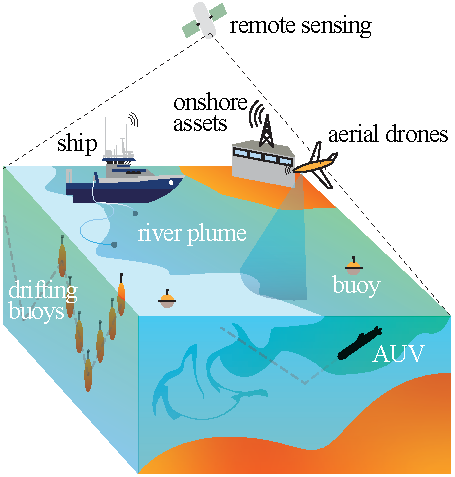
\includegraphics[width =
    0.48\textwidth]{Figures/envir.pdf}\label{fig:envir1}}
  \hfill
  \subfigure[Data-driven sampling under the sense-plan-act paradigm.]{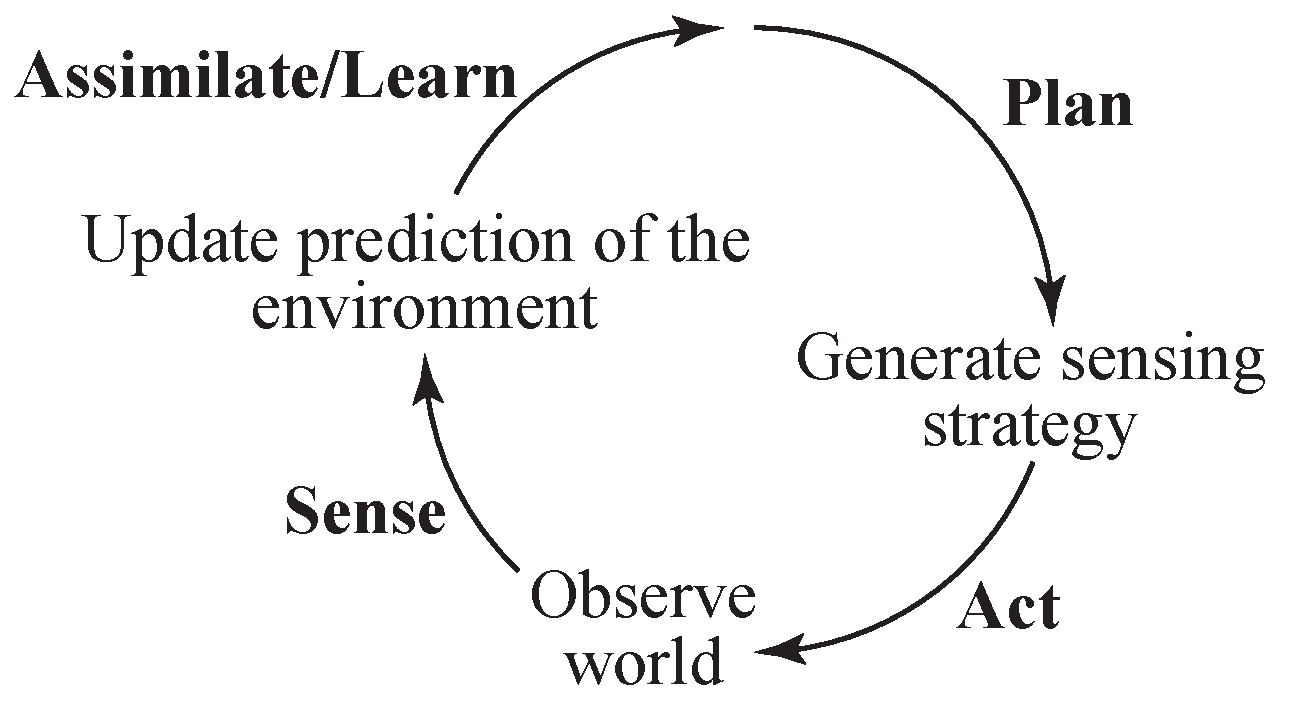
\includegraphics[width =
    0.48\textwidth]{Figures/adaptive_cycle.pdf}\label{fig:sense-plan-act}}
  \caption{Ocean observation is moving away from single-ship sampling
    towards more autonomous and collaborative networked operations in
    order to resolve the numerous bio-geochemical processes and their
    interactions.}
\label{fig:envir}
\end{figure}

Our focus in this work is towards spatial characterization of a
frontal system, more specifically, fronts generated by river
plumes. Fig. \ref{fig:nidelven} shows the survey area (the outlet of
the Nidelva river, Trondheim, Norway) where cold freshwater enters
from the river creating a strong gradient in both temperature and
salinity. Because of the local topography and the Coreolis force
\citep{coriolis1835memoire} the cold fresh water tends to flow near
land to the east. Depending on the river discharge, tidal effects,
wind, and temperature differences, this boundary often gets
distorted. Prior knowledge about the location and evolution of these
features is therefore highly uncertain, making deterministic planning
challenging.

\begin{figure}[!h] 
\centering 
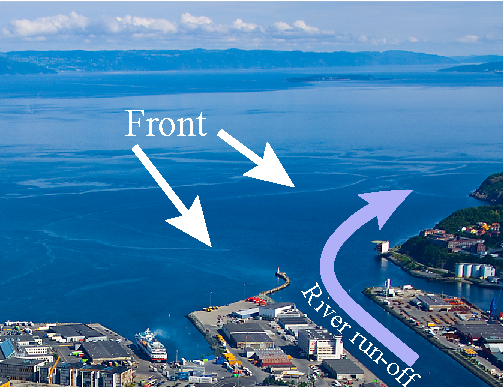
\includegraphics[width=0.85\textwidth]{Figures/pictures/c-updated.pdf}
\caption{Frontal patterns off of the Nidelva river, Trondheim, Norway.}
\label{fig:nidelven}
\end{figure}

%\begin{figure}[!h]
%\centering
 % \subfigure[River front - Columbia River, Astoria, Oregon, US.]{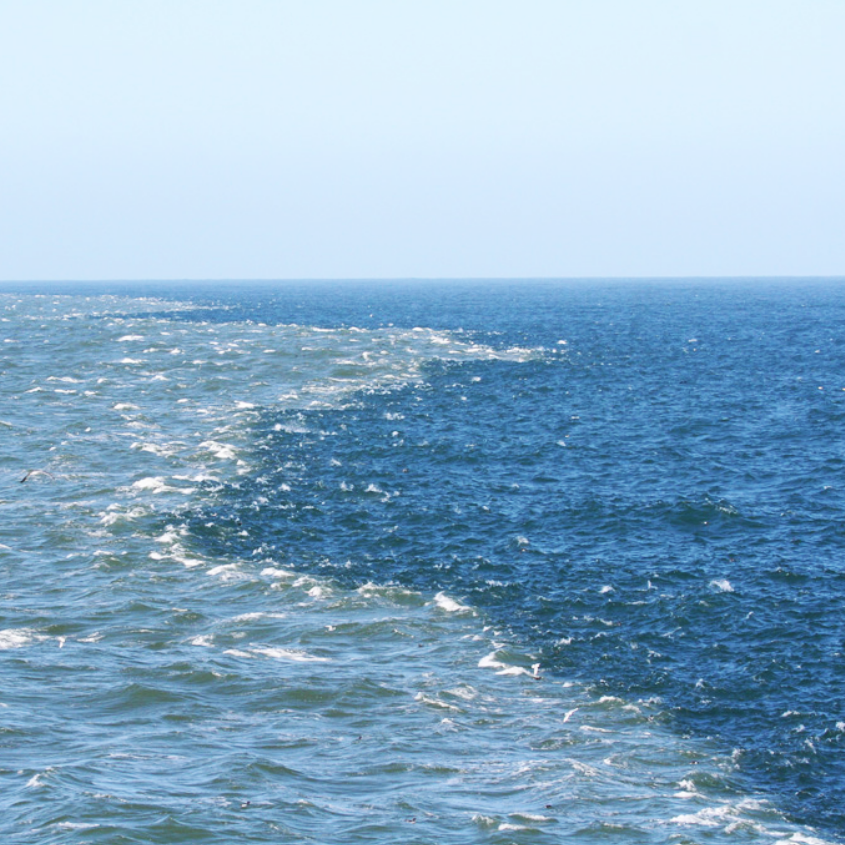
\includegraphics[width = 0.45\textwidth]{Figures/pictures/a.png}\label{fig:river1}}
 % \hfill
 %\subfigure[Tidal front - Korsfjorden, Norway.]{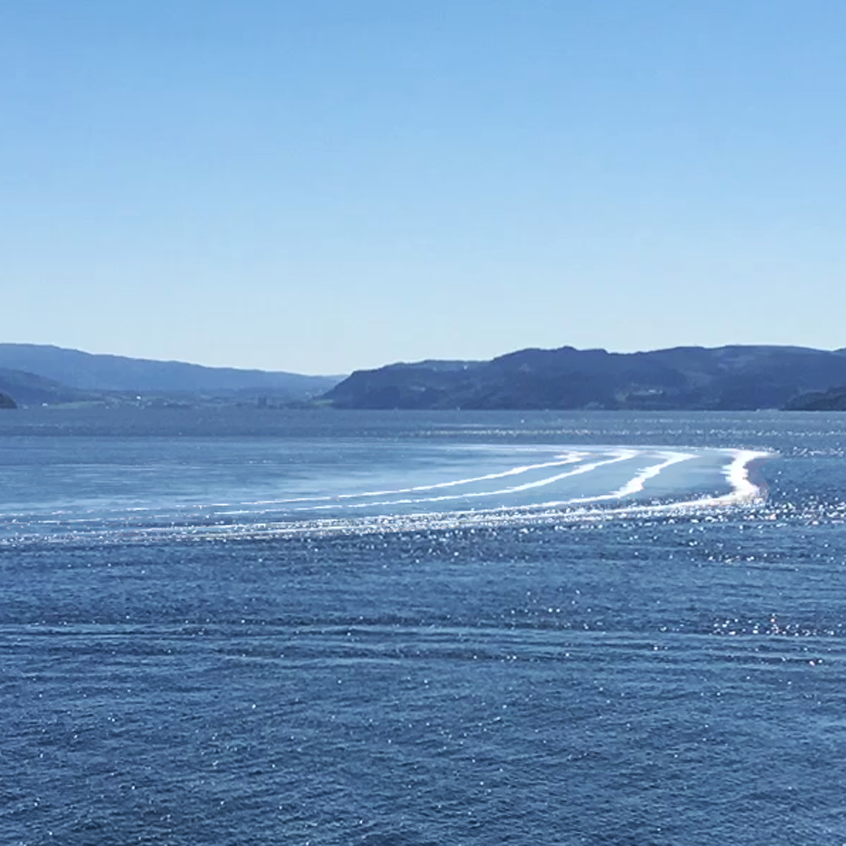
\includegraphics[width = 0.45\textwidth]{Figures/pictures/d.png}\label{fig:river2}}
 % \hfill
 % \subfigure[River plume - Rio de la Plata, Buenos Aires, Argentina.]{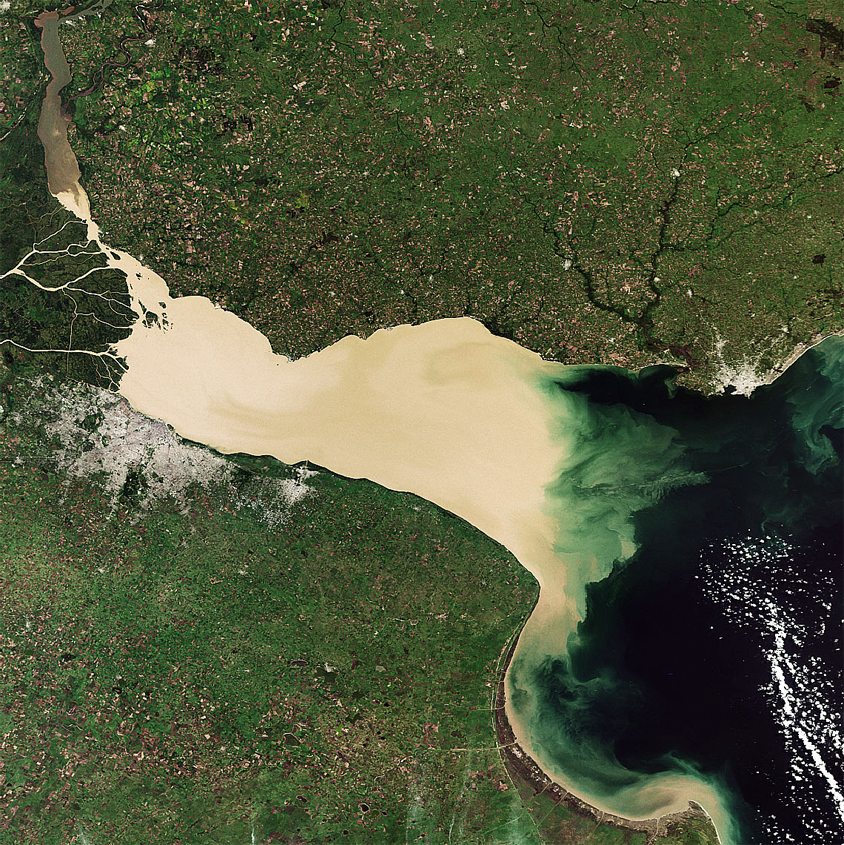
\includegraphics[width = 0.45\textwidth]{Figures/pictures/b.png}\label{fig:river3}}
 % \hfill
 %\subfigure[Frontal patterns - Nidelven, Trondheim, Norway.]{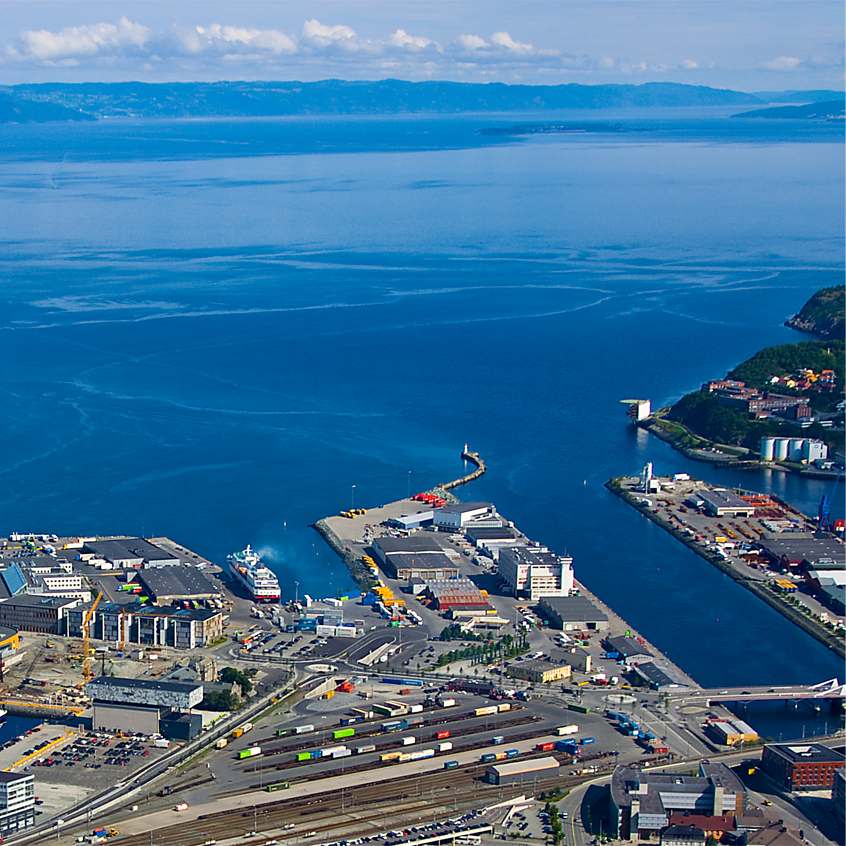
\includegraphics[width = 0.45\textwidth]{Figures/pictures/c.png}\label{fig:river4}}
 %\caption{Two examples of frontal features associated with
%   river-ocean interaction. % (\ref{fig:river1}) The river plume front of
   % the Columbia River meeting the Pacific Ocean.
%   (\ref{fig:river2})  Superimposed images (over 10 minutes) of a surface tidal front in
%   Korsfjorden, Norway. % (\ref{fig:river3}) The river plume of the Rio de
   % la Plata, taken by European Space Agency (ESA)'s Envisat platform and
   % MEdium Resolution Imaging Spectrometer (MERIS) sensor.
%   (\ref{fig:river4}) Aerial image of the mouth of the Nidelva river in
%   Trondheim, Norway where fresh water meets the salty fjord and creates
%   frontal patterns.} % Image courtesy: (\ref{fig:river1})
   % \cite{zamon2014marine}, (\ref{fig:river3}) ESA, CC BY-SA 3.0 IGO.}
% \label{fig:river_fronts}
%\end{figure}

%The use of \emph{robotic sampling} is motivated by the fundamental challenges of ocean observation, where a limited set of resources, a highly dynamic ocean, and the associated 

%This challenge can be addressed by employing more elaborate and adaptive sampling strategies that can capitalize on both prior and current observations in order to locate and map these areas.  

River plumes belong to a class of ocean processes that are local and
at smaller \emph{sub-mesoscale} (from $5 m^2$ -- $10 km^2$) where
spatial lateral variability tends to dominate. Remote sensing and
synthetic ocean models find it challenging to provide detail at this
scale \citep{Lermusiaux:2006} and the principal way to resolve for
fine resolution is by direct observation. At larger \emph{mesoscale}
($>50 km^2$), both three-dimensional space and time dynamics are
important and can shift substantially, while in the case of river
plumes one can often limit the scope to cover only lateral spatial
elements. Moreover, in this case, time-effects can be regarded as
static when acquiring AUV data over a short time window and limited
region. However, the methodological framework can be extended to
higher dimensional situations in a similar manner.

\subsection{Autonomous Vehicles}

AUVs are used to gather in-situ spatio-temporal data while carrying a range of scientific payloads to survey the
water column. Typically, they operate at $\sim 1-3$ m/s, can reach
depths from 100--6000 m with an in-water operation time capacity dependent on
survey speed, payload sensors and mission design. By deploying AUVs
together with other resources, one can augment information obtained
from ocean models, remote-sensing data, or fixed-location
sensors on buoys. Traditional operations and surveys with AUVs are
usually limited to observations along fixed transects on a spatial
grid, pre-programmed by the human operator. By instead using on-board
algorithms to continuously evaluate, update, and refine future
sampling locations, one can make information gathering adaptive and
contextual to the survey requirements
\citep{das11b,fossuminformation,fossum18b}. The space of sampling
opportunities is still limited to the spatial grid, but now there is
much more flexibility because of adaptation. For instance, an AUV
could reconstruct or modify a survey line based on what temperatures
it is measuring by using embedded methods in decision-theoretic
planning \citep{py10,Rajan12,Rajan12b}.

%To improve the state of sampling, modern tools and methods, including the use of autonomous platforms, oceanographic models and satellite remote sensing, needs to be combined with traditional data acquired by surface vessels or buoys (See Fig. \ref{fig:envir}). However, without adequate understanding of the theoretical underpinnings of how, when, and where to gather data, these tools and methods are insufficient in the vast and harsh oceans.

% retaining an advantageous strategy for information recovery, online during execution.
%The pressure on marine resources is growing and increased accuracy, resolution, and persistent monitoring of the oceans is crucial for long-term sustainable management. The impact of this research provides cost effective tools, techniques, and processes for doing ocean based measurements using robotic platforms. 
%adaptive design of experiments using robotic assets identifying and prioritizing relevant sampling locations on an information-theoretic basis. Spatial statistics naturally enters here through the ability to both model spatially correlated parameters and provide formal measures of uncertainty, on which this basis can be formed. 
%for oceanic sensing applications, where sensors are sparsely distributed and capitalizing on all available information is 

%This imperfect understanding of causality coupled with uncertainty implies that we need to obtain more measurements and use statistical models and methods to determine what and how phenomena form, to increase the quality of predictive statements. To improve the state of sampling, modern tools and methods, including the use of autonomous platforms, oceanographic models and satellite remote sensing, augment the more traditional data acquired by surface vessels or buoys (See Fig. \ref{fig:envir}). However, without adequate understanding of the theoretical underpinnings of how, when, and where to gather data, these tools and methods are insufficient in the vast and harsh oceans.

%There are several oceanographic data sources that can be used together with statistical tools to improve data collection in ocean science. In the following section we briefly discuss buoy data, satellite data, ocean models data, and AUV data.

%Buoy data provide very accurate information of oceanographic variables, but in most situations they are local, giving information only at one (north, east) coordinate, possibly with opportunities for conducting measurements at different depths. Gliders and other surface vessels are a kind of floating buoys that drift and can measure variables at many locations, but still with limited spatial coverage. 

%Satellite data are important for the mapping of oceanographic variables. They can also be indicative of variables such as temperature and salinity which we look at here, especially if the data are calibrated to for instance buoy data from the same spatial domain. However, the resolution of satellite data is relatively large, say $1 \times 1$ km $^2$ grid cells, and it only provides accurate information at the sea surface. Moreover, one cannot get useful satellite information on a cloudy day. 

%What is often done in practice is to run ocean models based on the complex differential equations governing oceanographic phenomena, where also satellite data can be assimilated and used as input, and possibly playing with different forcing mechanisms to capture some of the uncertainty of the models. Initial conditions, and can be used t the goal is to guide the sampling towards regions these regions, where we can reduce the uncertainty in the ES. These models provide insight that can be understood from practitioners, but they tend to be biased, and must also be calibrated to buoy data in one way or the other.

%to provide an effective specification of regions of phenomenological interest resolving the boundaries and the position of phenomena, on which evaluation of future sampling can be constructed.

%; some of these phenomena are illustrated in Fig. \ref{fig:envir2}. Figure \ref{fig:river_fronts} illustrates the %phenomena of interest in this paper, which is river plumes and their interaction with the ocean.

%Feature driven sampling
%processes acting across a wide range of spatio-temporal scales makes prioritizing sampling efforts necessary. %Autonomous robotic platforms, can address these issues by providing the ability to focus sampling efforts to %high-interest regions (``hotspots").


% Determining paths for mobile robotic sensors in order to maximize the
% information gained about an environment is formally known as informative
% path planning. This, and related problems such as the orienteering
% problem \citep{Golden87}, has been studied in the context of graphs,
% where the potential measurement are assigned to nodes on which
% evaluation of different routes can be conducted.
%In this context, a fundamental result from \cite{nemhauser1978analysis} proves that a simple greedy algorithm (iteratively selecting the location which most increases the utility) can achieve a near-optimal solution if the problem can be shown to be \emph{submodular}\footnote{an intuitive diminishing returns property, where the informative value of adding sensors decrease with the number of sensors added.}. Building on this result, \cite{chekuri2005recursive} explored this in the setting of a graph using a recursive greedy algorithm, providing near-optimal solutions depending on the planning horizon and graph resolution. 

Adaptive sampling of an evolving frontal feature has been explored in
\cite{fronts11,Zhang2012,Pinto2018,costa19}. These approaches
typically use a reactive-adaptive scheme, whereby exploration does not
rely on a statistical model of the environment, but rather adapts
based on closing the sensing and actuation loop
(Fig. \ref{fig:sense-plan-act}). Myopic sampling—i.e. step-wise
selection of the path (on the graph) which reduces the information
criterion the most—has been used for adaptive surveys
\citep{singh2009efficient,Binney2013} that focus largely on reducing
predictive variance or mutual information (e.g. entropy). Variance and
entropy reduction are independent of the actual data realizations
under the assumptions of GP models; the use of data-driven adaptive
criteria was introduced to include more targeted sampling of regions
of scientific interest in \cite{Low2009} and \cite{fossuminformation}.
In this paper, with a focus on mapping the river plume, we reward
the designs that improve the classification of water masses as a
means to characterize the frontal zone.

%\begin{figure}[h]
%\centering
%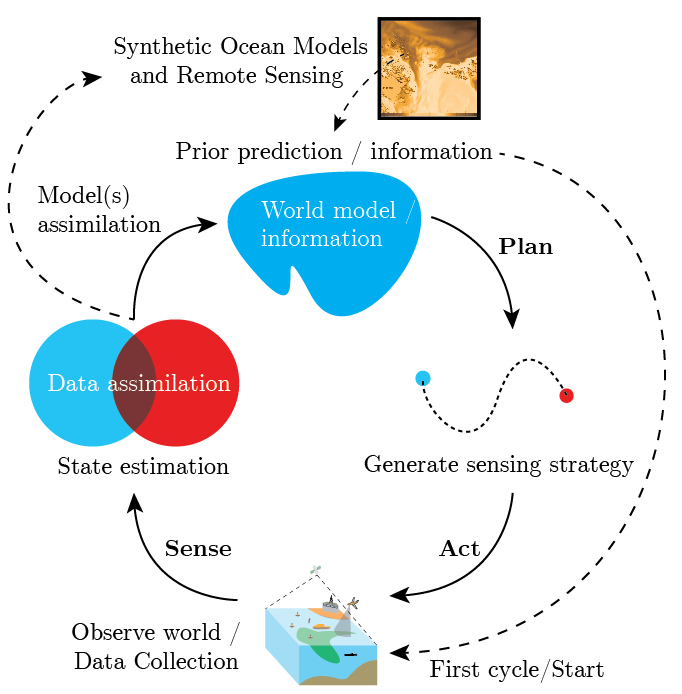
\includegraphics[width=0.4\textwidth]{Data-driven.png}
%\label{fig:auv_alone}
%\caption{The concept of data-driven sampling.}
%\end{figure}

%The goal is effectively map the extension of the river plume given this


%, we can formulate this question as follows: the ocean region  defined by the boundary between water bodies, separated by a characteristic temperature gradient that is smaller than $T=5$\textdegree C and a salinity concentration lower than $S=30$ [g/kg]. A goal is then to improve our predictive capabilities to answer this question better.
%For example,  (examples are shown in Fig. \ref{fig:river_fronts}). However, 

% In doing so, the aim is to increase the knowledge about the uncertain ocean environment through adaptive sampling


\section{Excursion Sets and Integrated Bernoulli Variance}
\label{sec:ESEP}

Our objective is to leverage statistical tools to characterize a river plume, focusing on spatial separation of cold freshwater from the river and warmer saline waters of the fjord. Excursion sets (ES) and excursion probabilities (EP) are useful starting points to measure the ability to classify water masses. The goal of experimental sampling is to improve this characterization, as quantified via changes in the EPs.

We consider a lateral domain near the sea surface, with locations
$\bx \in \mathcal{M} \subset \mathbf{R^2}$. The two variables of
interest, temperature and salinity, are defined as random processes:
$\xi_T(\bx)$ denotes the temperature (in $^o C$) and $\xi_S(\bx)$
denotes the salinity (in $mg/l$) at location $\bx$. The generalization to more than two variables is given in Section \ref{gen_k}. 

We let $t_T$ be a threshold for temperature and $t_S$ a threshold for salinity. The joint ES is then defined by:
\begin{equation}\label{ES}
     \mbox{ES} = \{\bx \in \mathcal{M} | \xi_T(\bx) \leq t_T,\xi_S(\bx) \leq t_S\}.
\end{equation}
The excursions could also be defined as larger than a threshold, or
within a boundary of limits for the two variables; calculations and
interpretations will be similar in these cases.

The ES holds random indicator variables while the associated EPs are: 
\begin{equation}\label{eq:prob}
  p(\bx) = P(\xi_T(\bx) \leq t_T, \xi_S(\bx) \leq t_S), \hspace{3mm} \bx \in \mathcal{M}.
\end{equation}
If the EPs in Eq. (\ref{eq:prob}) are
close to $1$ or $0$ at a given location, it is easy to classify water mass at this point as either river or ocean; it is, however,
challenging if the probability is close to $0.5$. 
The integrated Bernoulli variance (IBV) \cite{bect2019}, is defined as: 
\begin{equation}\label{measVAR}
    V = \int_{\bx \in \mathcal{M}} p(\bx) \left(1-p(\bx)\right) d\bx.
\end{equation}

If prior knowledge provides a strong indication of cold freshwater
 in a part of the domain, it is easy to classify and
there is likely little value in exploring those locations. Data can be
gathered at selected locations of the domain $\mathcal{M}$, to improve
classification performance. We denote temperature measurements by
$y_{T}(\bx_i)$ and salinity measurements by $y_{S}(\bx_i)$ at a
sampling location $\bx_i \in \mathcal{M}$. Given a set of
measurements denoted $\by$, the conditional EPs are:
\begin{equation}\label{eq:post_ep}
 p(\bx;\by) = P(\xi_T(\bx) \leq t_T, \xi_S(\bx) \leq t_S |\by). 
\end{equation}

Our goal is to construct adaptive sampling strategies based on continuous evaluation of the EPs. As the EPs provide a description of the boundary uncertainty, the strategies can effectively use this description to prioritize sampling efforts at locations that are ambiguous, making exploration more effective. As the AUV gathers data throughout its mission, it is natural to evaluate the expected reduction in the IBV, conditioned on the survey data. In this way, we can
take the expectation with respect to the planned measurements $\by$
\begin{equation}\label{sur}
    V_{\mbox{upd}} = \int_{\bx \in \mathcal{M}} E_{\by} \left\{ p(\bx;\by)\left( 1-p(\bx;\by)\right) \right\} d\bx, 
\end{equation}
where the expectation is over the planned data, and the probability is defined in Eq. (\ref{eq:post_ep}).
Considering a set $\mathcal{J}$ of possible designs for an AUV survey, a criterion for the selection is
\begin{equation}\label{crit}
    j^* = \mbox{argmin}_{j \in \mathcal{J}} V_{\mbox{upd}}(j),
\end{equation}
where the criterion $V_{\mbox{upd}}(j)$ in Eq. (\ref{sur}) is computed
for each of the possible designs. 

Recent work on ESs and EPs connected to spatial statistics include
\cite{picheny2010,french2013spatio,bolin2015excursion,french2016credible}.
Our focus is on ES as defined in Eq. (\ref{ES}) and the uncertainty
reduction achieved by sampling as in Eq. (\ref{sur}). In this sense,
our work is similar to \cite{bect2012}, \cite{chevalier2014fast} and
\cite{azzimonti2016quantifying} who describe analytical results for
uncertainty reduction in ESs for univariate processes. A major
contribution of our work is to derive closed-form results for this
design criteria for situations where the underlying model is based on multivariate GPs.

\section{Gaussian Processes and Excursion Probabilities}
\label{sec:GP_EP}

Calculations of the EPs and the IBV require a model specification. We use Gaussian modeling, which provides a practical and popular probabilistic approach to modeling environmental data, allowing a closed form
evaluation of the IBVs, as derived in Section \ref{sec:sur}.

\subsection{Bivariate Gaussian Processes}

The Gaussian model is used to represent the bivariate random fields of temperature and salinity. At location $\bx \in \mathcal{M}$, the prior bivariate distribution is:
\begin{equation}\label{gp_bar}
  \begin{bmatrix}\xi_T(\bx) \\
    \xi_S(\bx) \end{bmatrix}
 \sim N \left( 
\begin{bmatrix} \mu_{T}(\bx)\\
\mu_{S}(\bx)
\end{bmatrix},\begin{bmatrix}
\sigma_{T}^2(\bx) & \sigma_{T}(\bx) \sigma_S(\bx) \gamma(\bx)  \\
\sigma_{T}(\bx) \sigma_S(\bx) \gamma(\bx)  & \sigma_{S}^2(\bx) 
\end{bmatrix}
\right),
\end{equation}
where the notation refers to Gaussian (Normal) distributed variables
specified by the mean vector and covariance matrix. For the application
of tracking river plumes, the model parameters are specified from a short preliminary survey. The mean varies with location, capturing the variability near the river mouth, while the variance parameters and correlation between salinity and temperature are assumed to be constant for all locations and within each water mass. 

For the spatial dependence among variables, we assume a separable correlation function with the same decay for salinity and temperature,
which is not unrealistic for our case with a river plume as the decay is related to the common water masses (Sect \ref{sec:case_study}). We have:
\begin{equation}\label{gp_corr}
\mbox{Cov}(\xi_i(\bx),\xi_j(\bx')) = \rho(\bx,\bx') \sigma_i \sigma_j (\gamma +(1-\gamma )\delta_{ij}), \\
\end{equation}
for $i,j \in {T,S}$ and $\delta_{ij}=1$ if $i=j$ and $\delta_{ij}=0$
otherwise. Moreover, we assume stationary isotropic random fields a priori where the
correlation function $\rho(\bx,\bx')$ solely depends on $\bx$ and
$\bx'$ via a Euclidean distance measure $h=\sqrt{||\bx-\bx'||^2}$. With
data and prior knowledge one could possibly fit and estimate
parameters of non-stationary or non-isotropic covariance functions and
more complex multivariate spatial covariance functions
\citep{gneiting2010matern,genton2015cross}; however that is left for
future work.

We discretize the spatial domain
$\mathcal{M}$ to a set of $n$ grid locations
$\mathcal{M}_g = \{\bx_i, i=1,\ldots,n \}$, where each cell has area $\Delta$. The
grid is used for the waypoint graph setting the possible design locations. It is also used when solving integrals expressions in Eq. (\ref{measVAR}) and
(\ref{sur}) which are then approximated by sums over all grid cells.  Using vector
notation, we denote the Gaussian temperature and salinity variables on
the grid and its density function by: 
\begin{equation}\label{prior}
    \bxi = (\xi_T(\bx_1),\xi_S(\bx_1),\ldots,\xi_T(\bx_n),\xi_S(\bx_n))^t, \hspace{3mm}
    \bxi  \sim  N(\bmu, \bSigma) %\pi (\bxi) & =& \frac{1}{(2\pi)^{n}|\bSigma|^{\frac{1}{2}}}e^{-\frac{1}{2}(\bxi -\bmu)^T\bSigma^{-1}(\bxi-\bmu)}.
\end{equation}
%Here, $\pi(\bxi)$ is the joint density function of length $2 n$ vector $\bxi$, and
The length $2 n$ vector $\bmu$ holds the expected values of
temperature and salinity at the grid locations, while the
$2n \times 2n$ matrix $\bSigma$ holds the
variance-covariances of temperature and salinity variables at all grid
locations.

\subsection{Data model and updating of Gaussian processes}

Data is gathered by an AUV that can measure temperature and salinity
at a subset of locations on the defined grid. This can be done in a
static manner, where the survey design is pre-planned, or in a
sequential way with several rounds of data gathering. For the latter,
a round of data is gathered first, and then assimilated to get an
updated model. Then the updated model is used to design and select the
next round of measurements, and so on. We describe the model for one
round of data and the Gaussian formula for a single update. In Section
\ref{sec:heuristics} we discuss sequential data gathering in the
context of adaptive design of AUV measurements.

We denote the data at $n_y$ locations by
$\by=(y_{T,1},y_{S,1},\ldots,y_{T,n_y},y_{S,n_y})^t$, representing the
temperature and salinity measurements gathered at the first round of
nodes in the grid. The conditional model for the data, given the true temperature
and salinity, is described by: 
\begin{equation}\label{likelihood}
\by | \bxi \sim N( \bG \bxi, \bR), %\pi(\by | \bxi)= \frac{1}{(2\pi)^{m}|\bR|^{\frac{1}{2}}}e^{-\frac{1}{2}(\by -\bG\bxi)^T\bR^{-1}(\by-\bG\bxi)},
\end{equation}
where $\bG$ is an $2n_y \times 2n$ matrix holding '$1$'s on the
measurement indices on the grid and '$0$' otherwise. The size
$2n_y \times 2n_y$ covariance matrix $\bR$ contains diagonal entries
$r^2_T$ and $r^2_S$ which are measurement error variances of
temperature and salinity observations.

The GP mean and covariance in Eq. (\ref{prior}) are updated when more information is available. The
updated distribution for temperature and salinity variables on the
spatial grid, given survey data $\by$, is Gaussian with mean and
covariance: 
\begin{eqnarray}\label{gp_upd}
  \bm &=& \bm(\by) = \bmu+\bSigma \bG^t (\bG \Sigma \bG^t+\bR)^{-1}(\by-\bG \bmu),  \\
  \bA &=& \bSigma - \bSigma \bG^t (\bG \bSigma \bG^t+\bR)^{-1} \bG
          \bSigma.\nonumber
\end{eqnarray}

The updated bivariate distribution at a grid location $\bx \in
\mathcal{M}_g$ is then: 
\begin{equation}\label{gp_hat}
\begin{bmatrix}
\xi_T(\bx) \\
\xi_S(\bx)
\end{bmatrix}
 |\by
 \sim N \left( 
\begin{bmatrix} m_{T}(\bx)\\
m_{S}(\bx)
\end{bmatrix},\begin{bmatrix}
a_{T}^2(\bx) & a_{T,S}(\bx)  \\
a_{T,S}(\bx)  & a_{S}^2(\bx)  
\end{bmatrix}
\right),
\end{equation}
with entries $m_{\cdot}$ and $a_{\cdot}$ extracted from the conditional mean and covariance
expressions in Eq. (\ref{gp_upd}).

% The conditional mean $\bm$ will be important in the following
% derivation in Section \ref{sec:sur}.
The calculation of the design criterion in Eq. (\ref{sur}) requires
the marginal distribution of the data which is defined over $\bxi$ to
be $\by \sim N( \bG \bmu,\bG \bSigma \bG^t+\bR)$.  However, it turns
out that a simplified form of the calculation is possible because the
conditional mean in Eq (\ref{gp_hat}) is a linear (affine) function of
the data $\by$ and the covariance is not a function of the data.
Before knowing the data, the distribution of the conditional mean is
\begin{equation}\label{distxi} \bm \sim N(\bmu , \bPsi), \hspace{3mm}
  \bPsi=\bSigma \bG^t (\bG \bSigma \bG^t+\bR)^{-1} \bG \bSigma.
\end{equation} 
When considering only grid location $\bx$, we can
extract elements from its mean vector and covariance matrix to get the
bivariate distribution \begin{equation}\label{dist_mxi} 
  \bm(\bx) \sim N \left( \begin{bmatrix}
      \mu_{T}(\bx) \\
      \mu_{S}(\bx) \end{bmatrix}, \begin{bmatrix}
      \psi^2_{T}(\bx) & \psi_{T,S}(\bx)\\
      \psi_{T,S}(\bx) & \psi^2_{S}(\bx) \end{bmatrix} \right),
\end{equation}
which is important for the derivation of the closed form solution of the design criteria.

\section{Uncertainty reduction in excursion sets}
\label{sec:sur}

\subsection{Excursion probabilities for Gaussian processes}

Based on Gaussian modeling assumptions, the EPs can be computed at any
location $\bx$. Without additional data, Eq.  (\ref{eq:prob}) gives us:

\begin{eqnarray}\label{eq:prob_mv0}
 p(\bx) &=& P(\xi_T(\bx) \leq t_T, \xi_S(\bx) \leq t_S) \nonumber \\
 &=& \Phi_2 \begin{pmatrix} 
\begin{bmatrix} t_T\\
t_S
\end{bmatrix};
\begin{bmatrix} \mu_{T}(\bx)\\
\mu_{S}(\bx)
\end{bmatrix},\begin{bmatrix}
\sigma_{T}^2(\bx) & \sigma_{T}(\bx)\sigma_{S}(\bx) \gamma(\bx)  \\
\sigma_{T}(\bx)\sigma_{S}(\bx) \gamma(\bx)  & \sigma_{S}^2(\bx)  
\end{bmatrix}\end{pmatrix},
\end{eqnarray}
where $\Phi_2$ is the bivariate Gaussian cumulative distribution
function, and the mean and covariance entries are as defined in Eq. (\ref{gp_bar}).

When data $\by$ are available, Eq. (\ref{eq:post_ep}) similarly gives
us:
\begin{eqnarray}\label{eq:prob_mv}
 p(\bx;\by) &=& P(\xi_T(\bx) \leq t_T, \xi_S(\bx) \leq t_S |\by)
 \nonumber \\
 &=& \Phi_2 \begin{pmatrix} 
\begin{bmatrix} t_T\\
t_S
\end{bmatrix};
\begin{bmatrix} m_{T}(\bx)\\
m_{S}(\bx)
\end{bmatrix},\begin{bmatrix}
a_{T}^2(\bx) & a_{T,S}(\bx)  \\
a_{T,S}(\bx)  & a_{S}^2(\bx)  
\end{bmatrix}\end{pmatrix},
\end{eqnarray}
with parameters as defined in Eq. (\ref{gp_upd}) and (\ref{gp_hat}). Here, the probabilities would not only depend on the data but also on the data design defined via matrix $\bG$ in Eq. (\ref{likelihood}). We next derive results that ease comparison of several designs.

\subsection{Expected Integrated Bernoulli variance for bivariate models}

We will next derive closed form solutions to the expectation in
(\ref{sur}). The location index $\bx$ is suppressed to avoid overly
complex notation. We present new results for computing the expectation
$E_{\by}\left\{ \cdot \right\}$ which is the integrand of
Eq. (\ref{sur}).

A critical first element in the derivation is using the GP model and the
linear dependence on $\by$ in the conditional mean in
Eq. (\ref{gp_upd}). This results in a closed form Gaussian
distribution for the conditional mean in Eq. (\ref{dist_mxi}). The
high-dimensional inner integral in Eq. (\ref{sur}) then reduces to a
bivariate integral \citep{bhattacharjya2013value, chevalier2014fast},
with expectation over $\bm=(m_{T},m_{S})^t$.  We standardize the two
variables in Eq. (\ref{sur}), i.e.  $Z_T=\frac{\xi_T-m_{T}}{a_{T}}$,
$Z_S=\frac{\xi_S-m_{S}}{a_{S}}$, and then
\begin{eqnarray}\label{ytom}
   P(\xi_T \leq t_T, \xi_S \leq t_S|\by) &=& P \left( Z_T \leq\frac{t_T-m_{T}}{a_{T}}, Z_S \leq\frac{t_S-m_{S}}{a_{S}}|\by \right) \nonumber \\
   &=& \Phi_2 \begin{pmatrix} 
\begin{bmatrix} \frac{t_T-m_{T}}{a_{T}}\\
\frac{t_S-m_{S}}{a_{S}}
\end{bmatrix};
 \begin{bmatrix} 0\\
0
\end{bmatrix},\begin{bmatrix}
1 & \eta_{s,t}  \\
\eta_{s,t}   & 1  
\end{bmatrix}\end{pmatrix} \nonumber \\
&=& P(\xi_T \leq t_T, \xi_S \leq t_S|\bm),
\end{eqnarray}
where $\eta_{T,S} =a_{T,S}/(a_{T} a_{S})$.
Since the expression only depends on $\by$ via its affine function $\bm$, the expectation in Eq. (\ref{sur}) is reduced to a bivariate integral over $\bm$. 
Introducing $\pi(\bm)$ for the density
function of $\bm$, the expected Bernoulli variance becomes:
\begin{eqnarray}\label{eq:var2}
E_{\by}(p(1-p)) &=& E_{\bm}(p(1-p)), \hspace{3mm} p=P(\xi_T \leq t_T, \xi_S \leq t_S|\bm) \nonumber \\
E_{\bm}(p(1-p)) & = & \int p[1-p] \pi(\bm) d\bm, \nonumber \\
 &=& \int P(\xi_T \leq t_T, \xi_S \leq t_S|\bm)  \pi(\bm) d\bm \nonumber  \\
&-& \int P(\xi_T \leq t_T, \xi_S \leq t_S|\bm) P(\xi_T \leq t_T, \xi_S \leq t_S|\bm) \pi(\bm) d\bm. 
\end{eqnarray}
We will next extend results of \cite{chevalier2014fast} to solve for
these two parts (see also \cite{stroh} for such an extensions).

For the first part of the above, we have:
\begin{equation}\label{part1:phi2}
 \int P(\xi_T \leq t_T, \xi_S \leq t_S|\bm) \pi(\bm) d\bm= 
P \left( Z_{T} \leq \frac{t_T-m_{T}}{a_{T}}, 
Z_{S} \leq \frac{t_S-m_{S}}{a_{S}} \right), \nonumber
\end{equation}
where $\bZ=(Z_{T},Z_{S})$ is a bivariate zero-mean and unit-variance
Gaussian vector, with $\mbox{Corr}(Z_{T},Z_{S})=\eta_{T,S}$. Moreover,
$\bZ$ is chosen to be independent of $\bm$. Using Eq. (\ref{dist_mxi}) we have
\begin{equation}
    E(a_{T} Z_{T}+m_{T}-t_T) = \mu_{T}-t_T, \hspace{3mm}
    \mbox{Var}(a_{T} Z_{T}+m_{T}-t_T) = a^2_T+ \psi^2_{T}, 
\end{equation}
for the temperature part and the same holds for the salinity part. From this we get:
\begin{eqnarray}\label{two_parts0}
& P & \left( Z_{T} \leq \frac{t_T-m_{T}}{a_{T}}, 
Z_{S} \leq \frac{t_S-m_{S}}{a_{S}} \right) \\
&=& \Phi_2 \begin{pmatrix} 
\begin{bmatrix} 0\\
0
\end{bmatrix};
\begin{bmatrix} \mu_{T}-t_T\\
\mu_{S}-t_S
\end{bmatrix},\begin{bmatrix}
a^2_T+ \psi^2_{T} & a_{T,S}+\psi_{T,S}  \\
a_{T,S}+\psi_{T,S}   & a^2_T+ \psi^2_{T} 
\end{bmatrix}\end{pmatrix} \nonumber.
\end{eqnarray}

For the second part of the expression (\ref{eq:var2}), standardization
implies that: 
\begin{eqnarray}\label{part1:phi4}
&& \hspace{6mm} \int P(\xi_T \leq t_T, \xi_S \leq t_S|\bm) P(\xi_T \leq t_T, \xi_S \leq t_S|\bm) p(\bm) d\bm =  \\
&P& \hspace{-3mm} \left( Z_{1,T} \leq \frac{t_T-m_{T}}{a_{T}}, 
Z_{1,S} \leq \frac{t_S-m_{S}}{a_{S}},Z_{2,S} \leq \frac{t_T-m_{T}}{a_{T}}, 
Z_{2,S} \leq \frac{t_S-m_{S}}{a_{S}} \right). \nonumber
\end{eqnarray}
Here, $\bZ_1=(Z_{1,T},Z_{1,S})$, $\bZ_2=(Z_{2,T},Z_{2,S})$ are
independent bivariate zero-mean and unit-variance Gaussian vectors,
both with element-wise correlation $\eta_{T,S}$. Moreover, $\bZ_1$ and
$\bZ_2$ are chosen to be independent of $\bm$. Hence:
\begin{equation}
    \left(
    \begin{array}{cccccc}
         Z_{1,T} \\
         Z_{1,S} \\
         Z_{2,T} \\
         Z_{2,S} \\
         m_{T} \\
         m_{S}
    \end{array}
    \right)
\sim N \left(
\left(
    \begin{array}{cccccc}
    0 \\
    0 \\
    0 \\
    0 \\
          \mu_{T} \\
         \mu_{S} 
    \end{array}
    \right),
   \left[ 
      \begin{array}{cccccc}
        1 & \eta_{T,S} & 0 & 0 & 0 & 0  \\
        \eta_{T,S} & 1 & 0 & 0 & 0 & 0 \\
        0 & 0 & 1 & \eta_{T,S} & 0 & 0 \\
        0 & 0 & \eta_{T,S} & 1 & 0 & 0 \\
        0 & 0 & 0 & 0 & \psi^2_{T} & \psi_{T,S} \\
        0 & 0 & 0 & 0 & \psi_{T,S} & \psi^2_{S} 
    \end{array}
\right]
\right).
\vspace{0.2cm}
\end{equation}

The solution to the second part of the equation above, is then to
evaluate a four-variable cumulative distribution function associated
with Eqn. (\ref{part1:phi4}), accounting for the mean, variance and
covariances of $\bZ_1$, $\bZ_2$ and $\bm$ in the appropriate linear
combinations. Using vector-matrix formulations, we define linear
combinations:
\begin{equation}\label{Vcomb}
    \bV=\left[
    \begin{array}{cccccc}
        a_T & 0 & 0 & 0 & 1 & 0 \\
         0 & a_S & 0 & 0 & 0 & 1 \\
         0 & 0 & a_T & 0 & 1 & 0\\
         0 & 0 & 0 & a_S & 0 & 1\\
    \end{array}
    \right] 
    \left(
    \begin{array}{cccccc}
         Z_{1,T} \\
         Z_{1,S} \\
         Z_{2,T} \\
         Z_{2,S} \\
         m_{T} \\
         m_{S}
    \end{array}
    \right),
\end{equation}
and this in turn then becomes:
\begin{eqnarray}\label{part1:phi4_2}
&& P \left( Z_{1,T} \leq \frac{t_T-m_{T}}{a_{T}}, 
Z_{1,S} \leq \frac{t_S-m_{S}}{a_{S}},Z_{2,S} \leq \frac{t_T-m_{T}}{a_{T}}, 
Z_{2,S} \leq \frac{t_S-m_{S}}{a_{S}} \right)  \\
&=&  \Phi_4 
\begin{pmatrix} 
\begin{bmatrix} t_T\\
t_S \\
t_T \\
t_S
\end{bmatrix};
E( \bV),Var(\bV)
\end{pmatrix} \nonumber.
\end{eqnarray}

The multivariate cumulative probabilities in two and four dimensions
are fast to compute using methods of \cite{genz2009computation}.  In
the end, the first part in Eq. (\ref{two_parts0}) and the second in
Eq. (\ref{part1:phi4}) are computed for each location on the grid, and
summed over $\bx \in \mathcal{M}_g$, gives the design evaluation
criterion in Eq. (\ref{sur}). 

\subsection{Generalization to the multivariate case}
\label{gen_k}

In our application domain with the variables temperature and salinity,
the solutions to the complex integral equations for the expected IBV
are reduced to calculating bi-variate and four-variate cumulative
distribution functions for Gaussian vectors. For the more general
situation one would be interested in $K$ random fields. Say, in the
ocean sciences the variables could include chlorophyll or other
bio-geochemical quantities, in addition to temperature and salinity.

The equations derived in the previous section can then be generalized. Let
$\bxi(\bx)=(\xi_1(\bx),\ldots,\xi_K(\bx))$, and the expected Bernoulli
variance is:
\begin{equation}\label{two_partsK}
E_{\by}(p(\bx;\by)(1-p(\bx;\by))), \hspace{3mm} p(\bx;\by)=P(\xi_k(\bx) \leq t_k ; k=1,\ldots,K|\by). 
\end{equation}
By the first key result of linear combination of Gaussian variables,
we reduce the integral to a $K$ dimensional integral of the relevant
$\bm=E(\bxi(\bx)|\by)$. Next, reducing the integral to two parts, we
standardize the variables and compute cumulative distributions.  In
summary, we get:
\begin{equation}\label{two_parts}
E_{\by}(p(\bx)(1-p(\bx))) =  \Phi_K 
\begin{pmatrix}
\begin{bmatrix} t_1\\
\vdots \\
t_K 
\end{bmatrix};
\bmu,\bA+\bPsi 
\end{pmatrix}
- \Phi_{2K} 
\begin{pmatrix}
\begin{bmatrix} t_1\\
\vdots \\
t_K \\
t_1\\
\vdots \\
t_K 
\end{bmatrix};
E(\bV),Var(\bV) 
\end{pmatrix},\nonumber
\end{equation}
where $\bA$ and $\bPsi$ are direct $K$-variate extensions of the
matrices in Eq. (\ref{two_parts0}), and the matrix $\bV$ finds the
relevant linear combination of two independent vectors
$\bZ_l=(Z_{l,1},\ldots,Z_{l,K})$, $l=1,2$ and $\bm$, as an extension
of Eq. (\ref{Vcomb}).

\subsection{An Example}

We calculate EPs and the Bernoulli variance for a few bivariate
Gaussian distributions to illustrate the concepts articulated above.
Fig. \ref{illus_bivarDens} shows contour plots of three different
densities with increasing correlation $\gamma$ between temperature and
salinity.
\begin{figure}[h!] \centering
  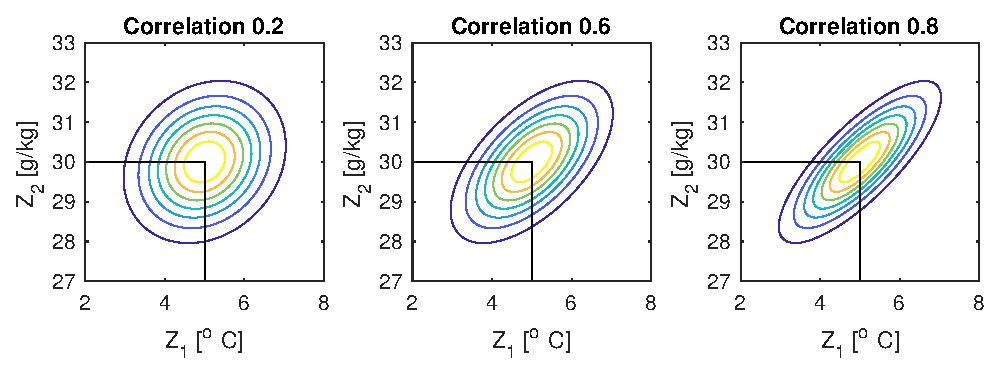
\includegraphics[width=0.99\textwidth]{Figures/illus_bivar.eps}
  \caption{Density contour plots having different correlations between
    temperature and salinity. The densities have unit variance and the
    thresholds are identical to the mean values $5^o C$ and
    $30 mg/l$. x-axis is temperature and y-axis is salinity.}
\label{illus_bivarDens}
\end{figure}
Here, the thresholds are set equal to the mean, $\mu_T=t_T=5^o C$ and
salinity $\mu_S=t_S=30$ mg/l. The displayed densities have unit
standard deviations for both temperature and salinity, but we also
study the effect of doubling the standard deviations.

Table \ref{tab:sim_rhoab} shows the EPs and the associated Bernoulli
variance (second row) for the examples indicated in
Fig. \ref{illus_bivarDens}. The EPs increase with the correlation as
there is a stronger tendency of having jointly small temperature and
salinity. The Bernoulli variance is similarly largest for high
correlation. EPs and Bernoulli variances are the same for standard
deviation $1$ or $2$, and this implies that high variability in
temperature and salinity is not captured in the $p(1-p)$ expression.

\begin{table}[!h] \centering \caption{EP and Bernoulli variance for
    different correlations and variances (top rows), and expected
    Bernoulli variances for both temperature and salinity data $\by$ and only for
    temperature $y_T$ (bottom rows).}
  \begin{tabular}{c|ccc|ccc}
 &\multicolumn{3}{c}{$\sigma_S=\sigma_T=1$} & \multicolumn{3}{c}{$\sigma_S=\sigma_T=2$} \\
\hline
Correlation $\gamma$ & 0.2 & 0.6 & 0.8 & 0.2 & 0.6 & 0.8 \\
\hline
$p$ & 0.28 & 0.35 & 0.40 & 0.28 & 0.35 & 0.40 \\ 
$p(1-p)$ & 0.20 & 0.23 & 0.24 & 0.20 & 0.23 & 0.24 \\ 
$E_{\by}(p(\by) (1-p(\by)))$ & 0.092 & 0.089 & 0.085 & 0.052 & 0.051 & 0.049 \\ 
$E_{y_T}(p(y_T) (1-p(y_T)))$ & 0.151 & 0.138 & 0.123 & 0.137 & 0.114 & 0.093 \\ 
\hline
\end{tabular}
\label{tab:sim_rhoab}
\end{table}

Table \ref{tab:sim_rhoab} (bottom two rows) shows results of expected
Bernoulli variance calculations. This is presented for a design
gathering both data types $(y_T,y_S)$, and for a design with
temperature measurements $y_T$ alone. Having both data;
$(y_T,y_S)^t=(\xi_T,\xi_S)^t+N(0,0.5^2\bI)$, while
$y_T=\xi_T+N(0,0.5^2)$ when only temperature is measured.  For this illustration, Table \ref{tab:sim_rhoab} shows that the expected Bernoulli variance
gets lower with larger standard deviations $\sigma_T$ and $\sigma_S$
(right columns). The reduction of Bernoulli variance is largest
for the cases with high correlation $\gamma$. Albeit smaller, there is
also uncertainty reduction when only temperature is measured (bottom
row), especially when temperature and salinity are very
dependent. When correlation is low ($\gamma=0.2$) there is little
information about salinity in the temperature data, and hence less
uncertainty reduction. In an application with fresh cold water from
river source, the temperature and salinity variables will not only be
interdependent, but will show dependence in the spatial
dimension. This in turn will impact the design criteria when we
evaluate the information measure by integrating over several locations
$\bx$.

%\subsection{Expected classification criteria}

%{\bf{I have not done anything here - skip this, I think}}.

%Rather than minimizing expected variance one can aim at minimizing the classification probability of the excursion set: 
%$\min [p,(1-p) ]$, see e.g. \cite{lilleborge2016information}. 

%Again, since the conditional mean is a linear in the data, we only have to look at the %relevant linear combination via $\bm_{\xi}=E(\bxi)$.
%See also \cite{bhattacharjya2013value}.

%\begin{equation}
%E(\min \{ p,(1-p)\})=\int \min P(\xi_T \leq t, \xi_S \leq s),[1-P(\xi_T \leq t, \xi_S \leq s)] p(E(\bxi)=) dE(\bxi)=,
%\end{equation}
%for the complementary probabilities, this is again evaluated by the corner regions for the block, and $\Phi_4()$ evaluations are required.

%In the end, this result is integrated over the spatial domain $x \in X$.

\section{Sequential updating and heuristic path planning}\label{sec:heuristics}

An important synergy underlining this work is the potential of robotic sampling to adapt survey plans based on data and statistical inference,
in accordance with the sense-plan-act loop
(Fig. \ref{fig:sense-plan-act}). We will therefore present a few adaptive strategies
for robotic sampling that builds on the notion of multivariate ES. Simulations, analysis, and  results from full-scale trials are presented.

\subsection{Optimal sequential design}
\label{Optdes}

An adaptive AUV survey is split in many rounds (stages), and at each
round, the survey design is found by using a myopic approach of
considering the largest reduction in uncertainty of the ES. In our
setting the selection is made on the graph defined by the nearest grid
nodes in the domain $\mathcal{M}_g$.

The optimal sequential design not only considers the best current AUV
grid node, but also what data gathered at this node would lead to for
future sampling at successive stages.  Let $d^{j,s}$ denote design
number $j$ at stage $s$ of a sequential survey. If this design is
selected, data $\by^{j,s}$ will be gathered. The optimal path
selection situation is then depicted in Figure \ref{fig:PathSelOpt},
\begin{figure}[h!]
\centering
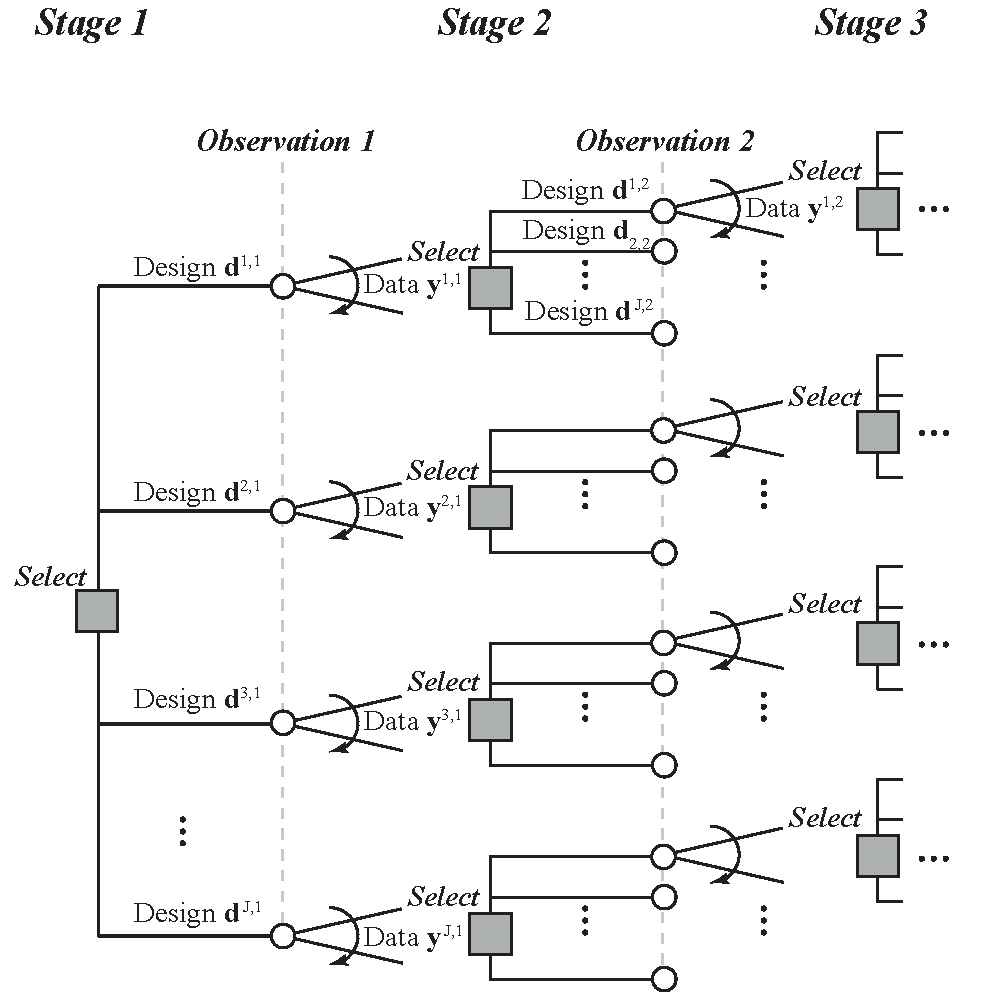
\includegraphics[width=0.85\textwidth]{Figures/sequent_select.pdf}
\caption{Optimal sequential path selection.}\label{fig:PathSelOpt}
\end{figure}
where design choices are indicated by squares while data realizations are indicated by circles. 
%terms this optimal design is defined as
%\begin{equation}\label{opt_crit}
%    \bd^* = \mbox{argmin}_{d^{j,1}} \left\{ \int_{\by^{j,1}} \mbox{argmin}_{d^{j,2}} \left\{ \int_{\by^{j,2}} \ldots \pi(\by^{j,2}|\by^{j,1}) d\by^{j,2} \right\} \pi(\by^{j,1}) d \by^{j,1} \right\},
%\end{equation}
%where $\ldots$ represents the expected variance reduction in the ES under the continued optimal design, which will depend on the data at earlier stages. 
The mathematical expression for the optimal design then involves a
series of intermixed maximizations over designs and integrals over
data.  In practice the optimal solution is not tractable because of
the enormous growth over stages, see
e.g. \cite{sucar2015probabilistic} and \cite{powell2016perspectives}.
Instead, we outline heuristic strategies. In terms of notation, let
$\mathcal{Y}^{s-1} =\{d^{j,r}, \by^{j,r} ; r=1,\ldots,s-1 \}$ denote
the data gathered until stage $s-1$, using a selected design
$d^{j,r}$, $r=1,\ldots,s-1$.

The derived closed form solutions for the expected IBV are still
important building blocks when constructing the sampling designs as
they will be used to score the different adaptive designs. % Efficient
% calculation is important for using adaptive survey designs with
% robotic platforms.
 
\subsection{A Naive Sampling Strategy}
\label{naive}

The simplest heuristic for adaptive sampling is to choose the next
sampling location based on current EPs. The largest variance in
sampling locations is and indication of higher uncertainty; therefore
one selects the design location with an EP closest to $0.5$.

At stage $s$, based on the currently available data
$\mathcal{Y}^{s-1}$, we fit an updated Gaussian model from
Eq. (\ref{gp_upd}), with mean $\bm_{s-1}=E(\bxi|\mathcal{Y}^{s-1})$
and covariance matrix $\bA_{s-1}=\mbox{Var}(\bxi|\mathcal{Y}^{s-1})$.
The next round of measurements $\by^{j,s}$, can be gathered with
design $d^{j,s}$, $j=1,\ldots,J$, where $J$ indicates all possible AUV
trajectories from the current stage. The {\it{naive}} strategy then,
selects the design according to:
\begin{eqnarray}\label{critNaive}
    d^{*,s} &=& \mbox{argmin}_{j \in \{1,\ldots,J\}} |p(\bx_{d^{j,s}};\mathcal{Y}^{s-1})-0.5|, \\
    p(\bx;\mathcal{Y}^{s-1}) &=& P(\xi_T(\bx) \leq t_T, \xi_S(\bx) \leq t_S | \mathcal{Y}^{s-1}). \nonumber
\end{eqnarray}
This strategy does not account for the uncertainty in the temperature
or salinity variables, only if one design (node) has EPs closer to
$0.5$ (see Table \ref{tab:sim_rhoab}, line two). Neither does it
account for spatial correlation. This strategy lacks memory of where
it has been and where the uncertainty has been reduced and therefore
susceptible to local minimas.

\subsection{Myopic path planning}
\label{myopic}

The myopic (greedy) strategy which we present here is optimal if we
imagine taking only one more round of measurements. In this selection
strategy there is no anticipation of what the subsequent designs might
offer, beyond the first round.

Based on the currently available data $\mathcal{Y}^{s-1}$, we again
fit an updated Gaussian model, represented on the grid locations
covering the spatial domain.  The next round of measurements
$\by^{j,s}$, can be gathered with design $d^{j,s}$, $j=1,\ldots,J$,
indicating all possible AUV trajectories at the current stage. The
selected design is then:
\begin{eqnarray}\label{critSEQ}
    d^{*,s} &=& \mbox{argmin}_{j \in \{1,\ldots,J\}} \left\{ V_{m,\mbox{upd,j}} \right\},  \\
V_{m,\mbox{upd}} & \approx & \sum_{\bx \in \mathcal{M}_g} E_{\by^{j,s}|\mathcal{Y}^{s-1}} \left\{ p(\bx;\mathcal{Y}^{j,s})\left( 1-p(\bx;\mathcal{Y}^{j,s})\right) \right\} \Delta, \nonumber \\
    p(\bx;\mathcal{Y}^{j,s}) &=& P(\xi_T(\bx) \leq t_T, \xi_S(\bx) \leq t_S |\by^{j,s},\mathcal{Y}^{s-1}). \nonumber
\end{eqnarray}

Note that this strategy gives a sequential conditional version of the
formula in Eq. (\ref{sur}). Now $\mathcal{Y}^{s-1}$ is available, and
the expectation is with respect to the conditional density
$\pi(\by^{j,s}|\mathcal{Y}^{s-1})$. A similar closed form calculation
for expected IBV is hence applicable in Eq. (\ref{critSEQ}), using the
updated GP model from step $s-1$.  Once the data is collected for the
best design, the GP model is updated again. The mean $\bm_{s}$ and
covariance matrix $\bA_{s}$ are used to compute the next design at
stage $s+1$, and so on.

Even though this myopic strategy is non-anticipative, it still gives a
reasonable approach for creating designs in many
applications. Moreover, it is easily implemented on-board an AUV,
using the efficient approach for data updating of the GP model and the
calculation of the closed form expected IBV expressions for each
subsequent trajectory.


\subsection{Look-ahead trajectory planning}
\label{LA}

We now extend the myopic strategy to a look-ahead strategy which is
optimal when one can gather only two more rounds of measurements. In
addition to the next round of measurements $\by^{j,s}$, this
look-ahead strategy, anticipates the subsequent design $j_2$ with
data $\by^{j_2,s+1}$, when choosing the current design $d^{j,s}$.  The
selected design is:
\begin{eqnarray}\label{critLA}
    d^{*,s} &=& \mbox{argmin}_{j \in \{1,\ldots,J\}} \left\{ U_{la,\mbox{upd,j}} \right\},  \\
    U_{la,\mbox{upd},j} & = &  E_{\by^{j,s}|\mathcal{Y}^{s-1}} \left\{ \mbox{argmin}_{j_2 \in \{1,\ldots,{J}_2\}} \left[ V_{la,\mbox{upd},j_2} \right] \right\}, \nonumber \\
V_{la,\mbox{upd},j_2} & \approx & \sum_{\bx \in \mathcal{M}_g} E_{\by^{j_2,s+1}|\mathcal{Y}^{j,s}} \left\{ p(\bx;\mathcal{Y}^{j,s+1})\left( 1-p(\bx;\mathcal{Y}^{j,s+1})\right) \right\} \Delta, \nonumber \\
    p(\bx;\mathcal{Y}^{j,s+1}) &=& P(\xi_T(\bx) \leq t_T, \xi_S(\bx) \leq t_S |\by^{j_2,s+1},\mathcal{Y}^{j,s}). \nonumber
\end{eqnarray}
Here, $\mathcal{Y}^{j,s}=\{\by^{j,s},\mathcal{Y}^{s-1}\}$ and
$\mathcal{Y}^{j,s+1}=\{\by^{j_2,s+1},\mathcal{Y}^{j,s}\}$ represent
the sets of data variables, and the expectations are with respect to
the conditional densities $\pi(\by^{j,s}|\mathcal{Y}^{s-1})$ and
$\pi(\by^{j_2,s+1}|\by^{j,s},\mathcal{Y}^{s-1})$.

Because of the intermixed optimization and expectation, there is no
longer a closed form for the required integrals. Instead, we solve the
first expectation by Monte Carlo sampling of data $\by^{j,s}$ from its
conditional distribution. For each data sample, the second expectation
is solved using the closed form expressions for expected IBV from
Section \ref{sec:sur}.

Even though the strategy looks at two stages, it is only used to find
the current best design. When data is collected, the GP model is
updated, and the mean $\bm_{s}$ and covariance matrix $\bA_{s}$ are
used to compute the next design at stage $s+1$, now anticipating what
stage $s+2$ could offer, and so on.

This look-ahead approach is much more computationally demanding than
the myopic strategy, and for practical implementation we prune paths
in the evaluation of Eq. (\ref{critLA}). This means that we do not
compute all possible branches of the first two stages, as they are
indicated in Figure \ref{fig:PathSelOpt}. Instead, we use the myopic
strategy to rank the three best designs on the first stage alone, and
for each of these we undertake the look-ahead calculations.

\section{Simulation study}
\label{sec:simulations}

We now show results from tests performed to study the properties of
different static and sequential survey designs, in a realistic
simulated case. The context is mapping a freshwater plume defined by a
temperature and salinity gradient using an AUV.

\subsection{Modeling}

We use a bivariate GP model for temperature and salinity, where we
specify the prior mean:
\begin{equation}\label{m}
    \bmu(\bx)=E 
    \begin{bmatrix}
    \xi_T(\bx) \\
    \xi_S(\bx) 
    \end{bmatrix}=\begin{bmatrix} \mu_{T}(\bx)\\
\mu_{S}(\bx)
\end{bmatrix} 
= \begin{bmatrix} \beta_{T,0} + \beta_{T,1} x_{\mbox{East}} \\
\beta_{T,1} + \beta_{S,1} x_{\mbox{East}}
\end{bmatrix}.
\end{equation}
In this simulation setup, which is motivated by a real case, we expect
the eastern part of the domain to be cold freshwater. This situation
mimics that of a river mouth entering from the south, and the water
masses are pulled to the east. The actual trends are, in practice, set
from preliminary information or runs of oceanographic models \cite{fossuminformation} solving differential equations for hydrodynamic flow. In this
example the mean is specified by regression parameters $\beta_{T,1}=0.065$ and
$\beta_{S,1}=0.1$ for the slope with west coordinate and $\beta_{T,0}=5.8$
and $\beta_{S,1}=29.0$ for the intercept at a reference start map coordinate.

%The prior assumption used by the agent are $\tilde{\beta_{T,1}}=0.085$ and $\tilde{\beta_{S,1}}=0.138$, which assumes that the process is centered. 

The covariance is assumed to be stationary and separable for the two variables. 
The $2 \times 2$ pointwise covariance matrix is set to:
\begin{equation}\label{v0}
\bSigma(\bx)=\mbox{Var} 
\begin{bmatrix}
    \xi_T(\bx) \\
    \xi_S(\bx) 
    \end{bmatrix}=
\begin{bmatrix}
0.25^2 & 0.6 \cdot 0.25^2 \\
0.6 \cdot 0.25^2 & 0.25^2
\end{bmatrix}.
\end{equation}
The spatial correlation is of a Matern type:
\begin{equation}\label{v}
\mbox{Corr} 
\left(
\begin{bmatrix}
    \xi_T(\bx) \\
    \xi_S(\bx) 
    \end{bmatrix},
    \begin{bmatrix}
    \xi_T(\bx') \\
    \xi_S(\bx') 
    \end{bmatrix}
    \right)
    = \begin{bmatrix}
1 & 0.6  \\
0.6  & 1
\end{bmatrix}(1+\phi |\bx-\bx'|)\exp (-\phi |\bx-\bx'|),
\end{equation}
and $\phi=0.3$ indicates an effective correlation range of about $1200$ m. 
%Figure \ref{fig:stat_design} shows the contour lines for the EP for the reference. We notice the trend of increasing salinity and temperature to the west.  
We study sensitivity to the parameter specification in the results
below.  One realization of the random fields representing salinity and
temperature is shown in Figure \ref{fig:true_temp} and
\ref{fig:true_sal}. The true ES from this prior realization is shown
in Figure \ref{fig:ESet}.

\begin{figure}[!ht]
  \centering
  \subfigure[Simulated temperature.]{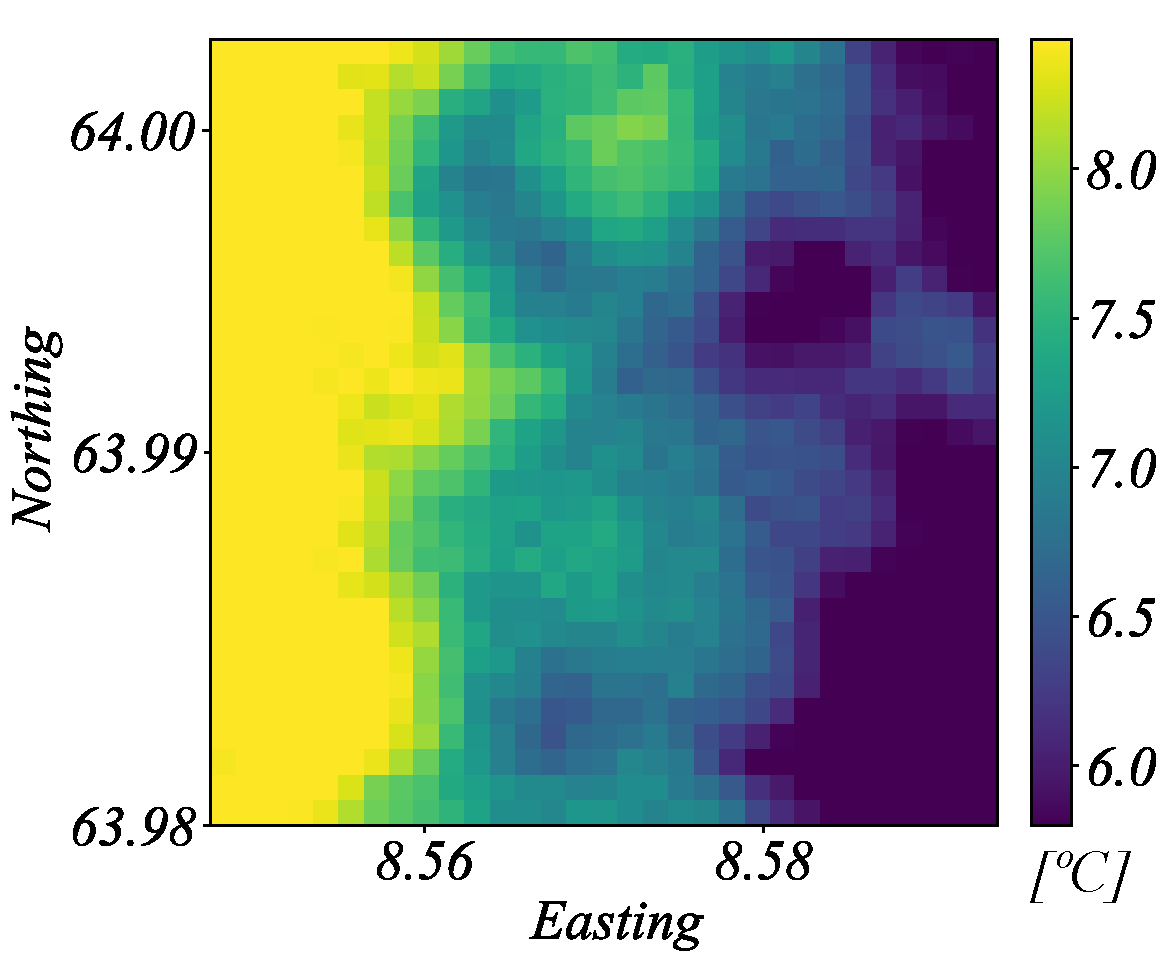
\includegraphics[height = 0.40\textwidth]{Figures/sim/true_temp.pdf}\label{fig:true_temp}}
  \hfill
  \subfigure[Simulated salinity.]{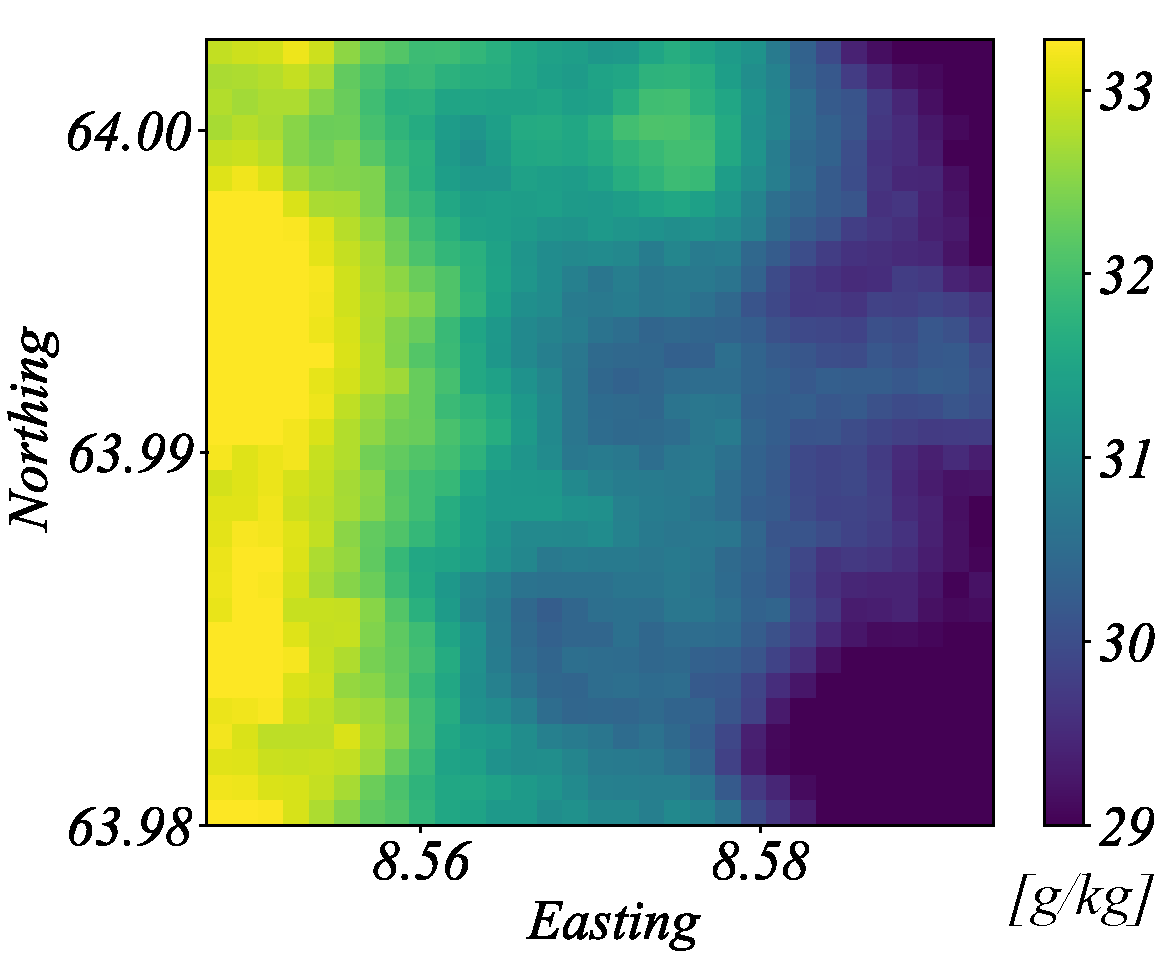
\includegraphics[height = 0.40\textwidth]{Figures/sim/true_sal.pdf}\label{fig:true_sal}}
  \hfill
  \subfigure[Excursion set given the realization of temperature and salinity.]{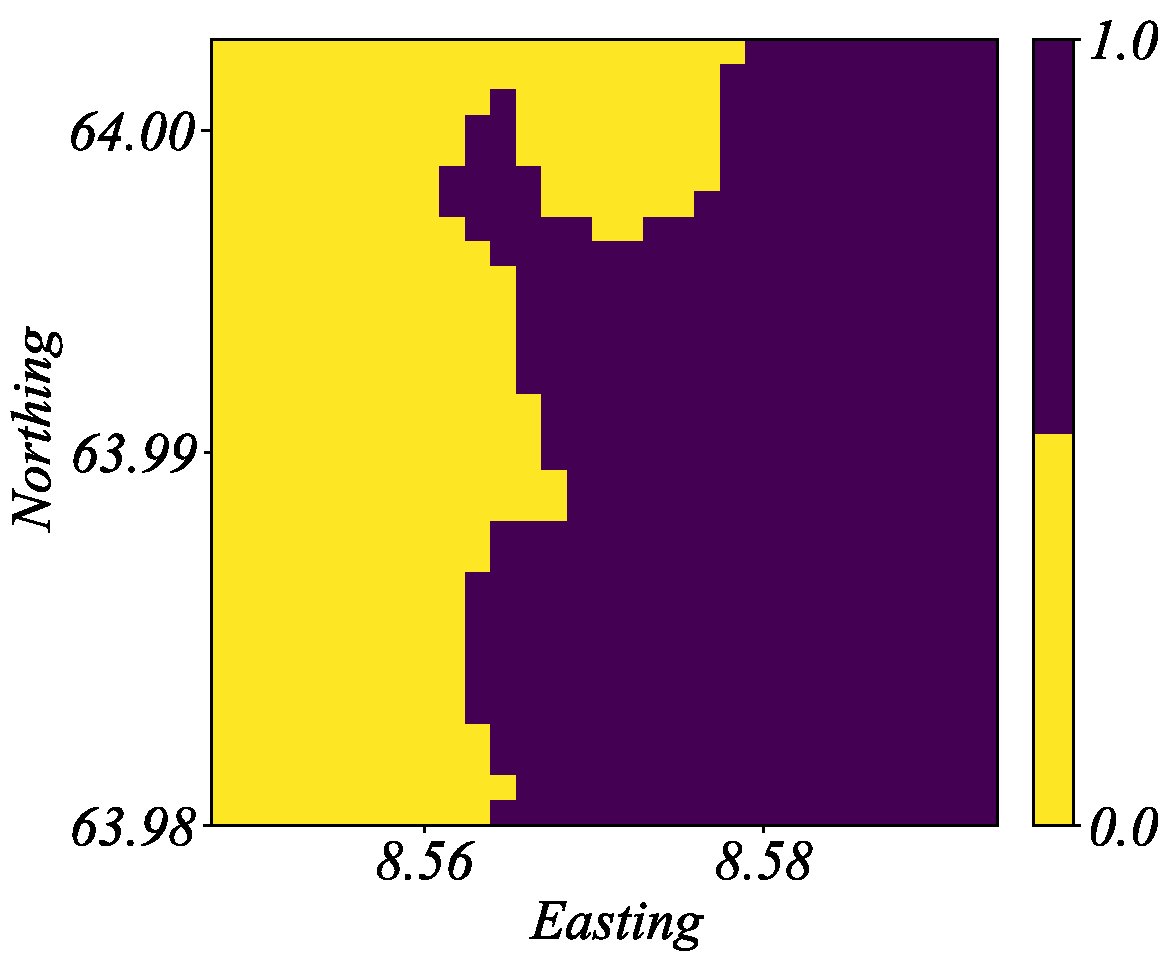
\includegraphics[height = 0.40\textwidth]{Figures/sim/es_ts_true.pdf}\label{fig:ESet}}
  \hfill
  \subfigure[Excursion probabilities given collected data using the
  `static\_north" strategy.]{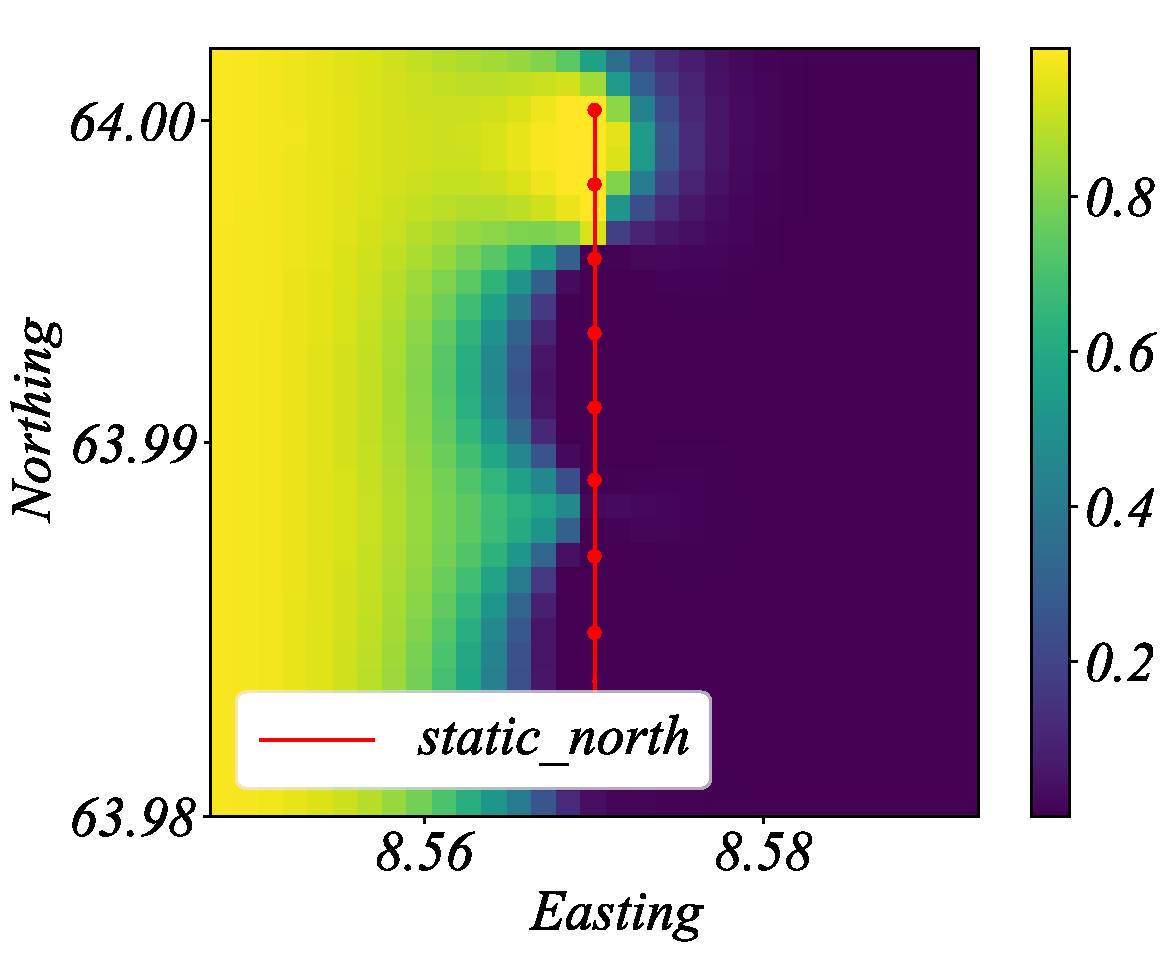
\includegraphics[height = 0.40\textwidth]{Figures/sim/es_ts_posterior.pdf}\label{fig:Eprob}}
  \caption{\ref{fig:true_temp} and \ref{fig:true_sal} show
    realisations of the simulated temperature and salinity fields, as
    well as the associated excursion set \ref{fig:ESet}.
    \ref{fig:Eprob} shows the estimated excursion probabilities after
    performing data collection along the N-S survey line.} 
\label{fig:realisations}
\end{figure}

\subsection{Static and sequential sampling designs}\label{sec:sampling_designs}

%Three different designs are considered as indicated in Figure \ref{fig:stat_design}. 
%\begin{figure}[h!]
%\centering
%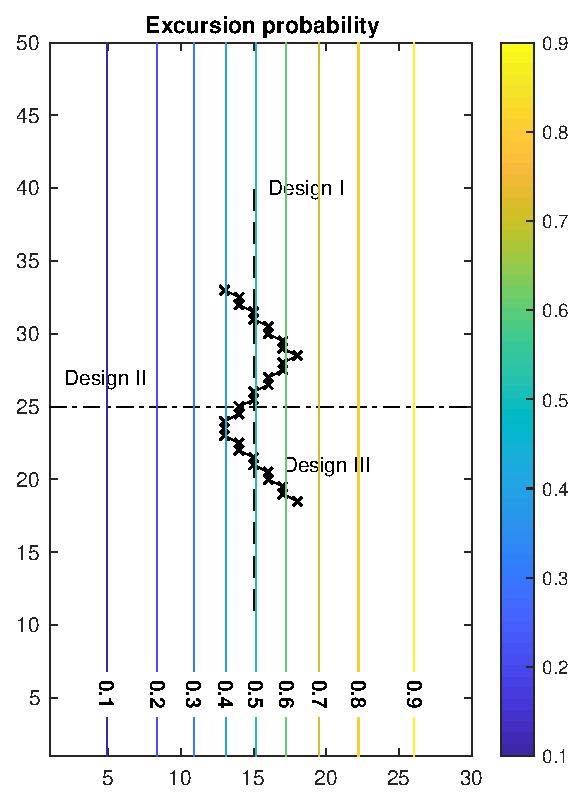
\includegraphics[width=0.65\textwidth]{Figures/Des3.eps}
%\caption{Three different static survey designs plotted on the initial EP.}\label{fig:stat_design}
%\end{figure}
%In this display the designs are plotted along with the prior probability contours of the ES for the reference parameter inputs. 

We compare three different static designs denoting
\texttt{static\_north}, \texttt{static\_east}, and
\texttt{static\_zigzag} with the three sequential approaches
\texttt{naive}, \texttt{myopic}, and \texttt{look-ahead}. The static
sampling paths are pre-determined and cannot be changed on the basis
of data, representing the typical pre-planned observation
strategies used in typical AUV operational survey designs.

For a fixed survey length, the expected variance is analytically available (equal coverage and reduction in variance each time). However, for the sequential approaches this is not the case, as the result and path are dependent on the observed data and the expected reduction in IBV. The properties is therefore evaluated using Monte Carlo sampling over several replicates of realizations from the prior, conducting simulated sequential surveying for each one. Figure \ref{fig:Eprob} shows the conditional EP, given data gathered along the north-south survey line for the realization indicated in these displays. In the Monte Carlo replicates, such results are repeatedly computed to approximate the expected variance reduction in the ES. We also compare predictive performance measured by root mean square error (RMSE) for the temperature and salinity estimates and the variance reduction in these two variables. It is important to note that the objective function used by the agents is focused on reducing the expected variance in the ES, but we nevertheless hope to achieve good predictive performance for criteria such as RMSE as well. Another non-statistical criteria that is important for practical purposes is the computational time of the strategy, as this will impact the performance of the approach in the field for an embedded system. 

\begin{figure}[h!]
\centering
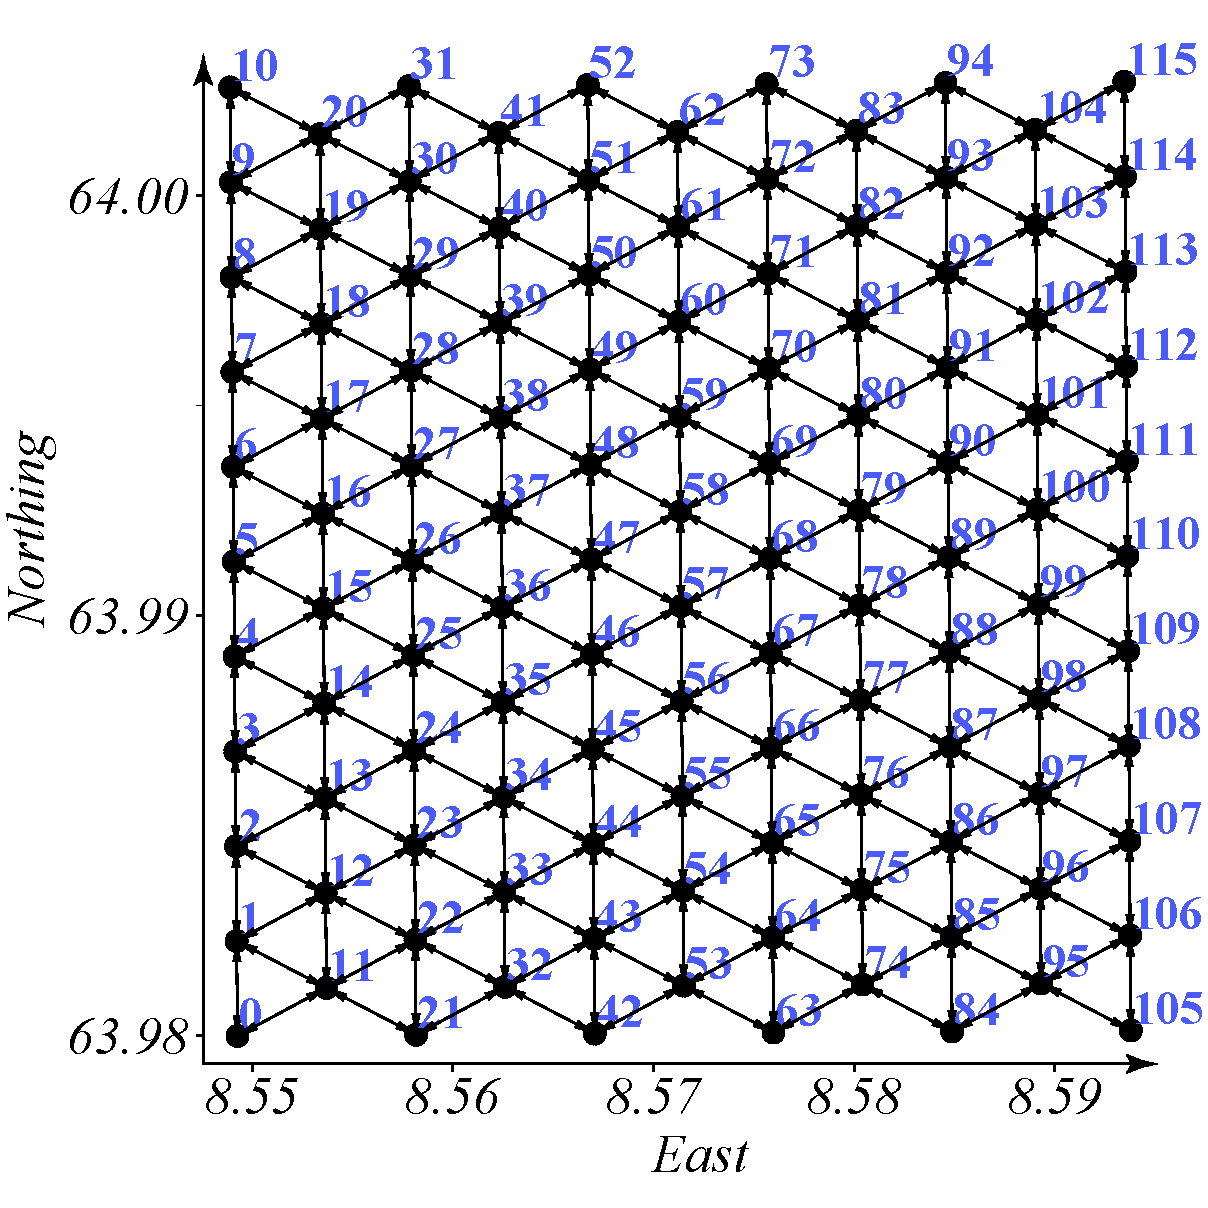
\includegraphics[width=0.50\textwidth]{Figures/sim/wp_graph_paper.pdf}
\caption{The equilateral waypoint graph used to discretize the
  trajectory choices over the $31\times31$ grid used to discretize the GP.}
\label{fig:wp_graph}
\end{figure}

Each strategy is conducted on an equilateral grid shown in Fig. \ref{fig:wp_graph}. The sequential sampling agents start at the center East-West coordinate at the southern end of the domain (node 53). The AUV will move along edges in the waypoint graph while the vehicle gathers measurements. The data is assimilated into the GP model, before an evaluation of the next node to sample is conducted at the end of the edge. The paths will differ for the various sequential designs due to the individual design criteria and the simulated variability in the environment among the replicates.

A total of 100 replicate simulation was conducted and the results are shown in Figure \ref{fig:sim_results},
where the different criteria are plotted as a function of survey distance. Figure \ref{fig:avg_ev} shows the resulting drop in ES variance for each of the six strategies. The ES variance is reduced most under the \texttt{myopic} and \texttt{look-ahead} strategies, performing almost equally; this is expected as the two criteria (Eq. \eqref{critSEQ} and \eqref{critLA}) are much more sensitive to differences in IBV. The north-south design also does well in terms of ES variance reduction since the path is parallel to the  boundary between the water masses.

\begin{figure}[h!]
  \centering
  % \subfigure[Excursion set variance $E_{\by}(p[1-p])$.]{\label{fig:avg_ev}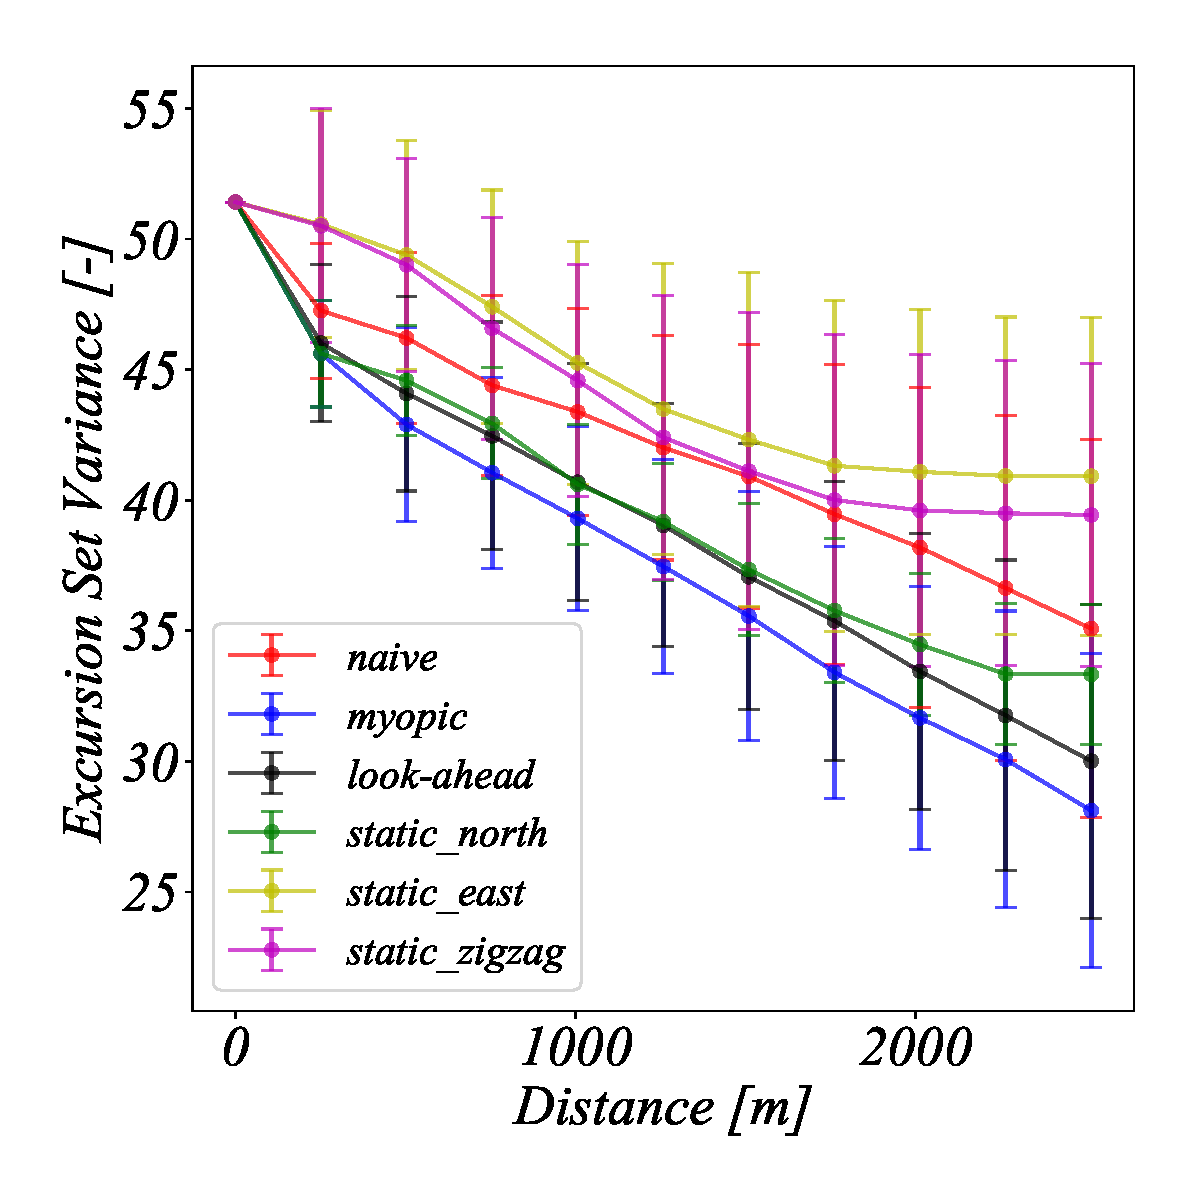
\includegraphics[height=0.49\textwidth]{Figures/sim/avg_EV.pdf}}
  \subfigure[Excursion set $E_{\by}$(p\lbrack 1-p\rbrack) variance.]{\label{fig:avg_ev}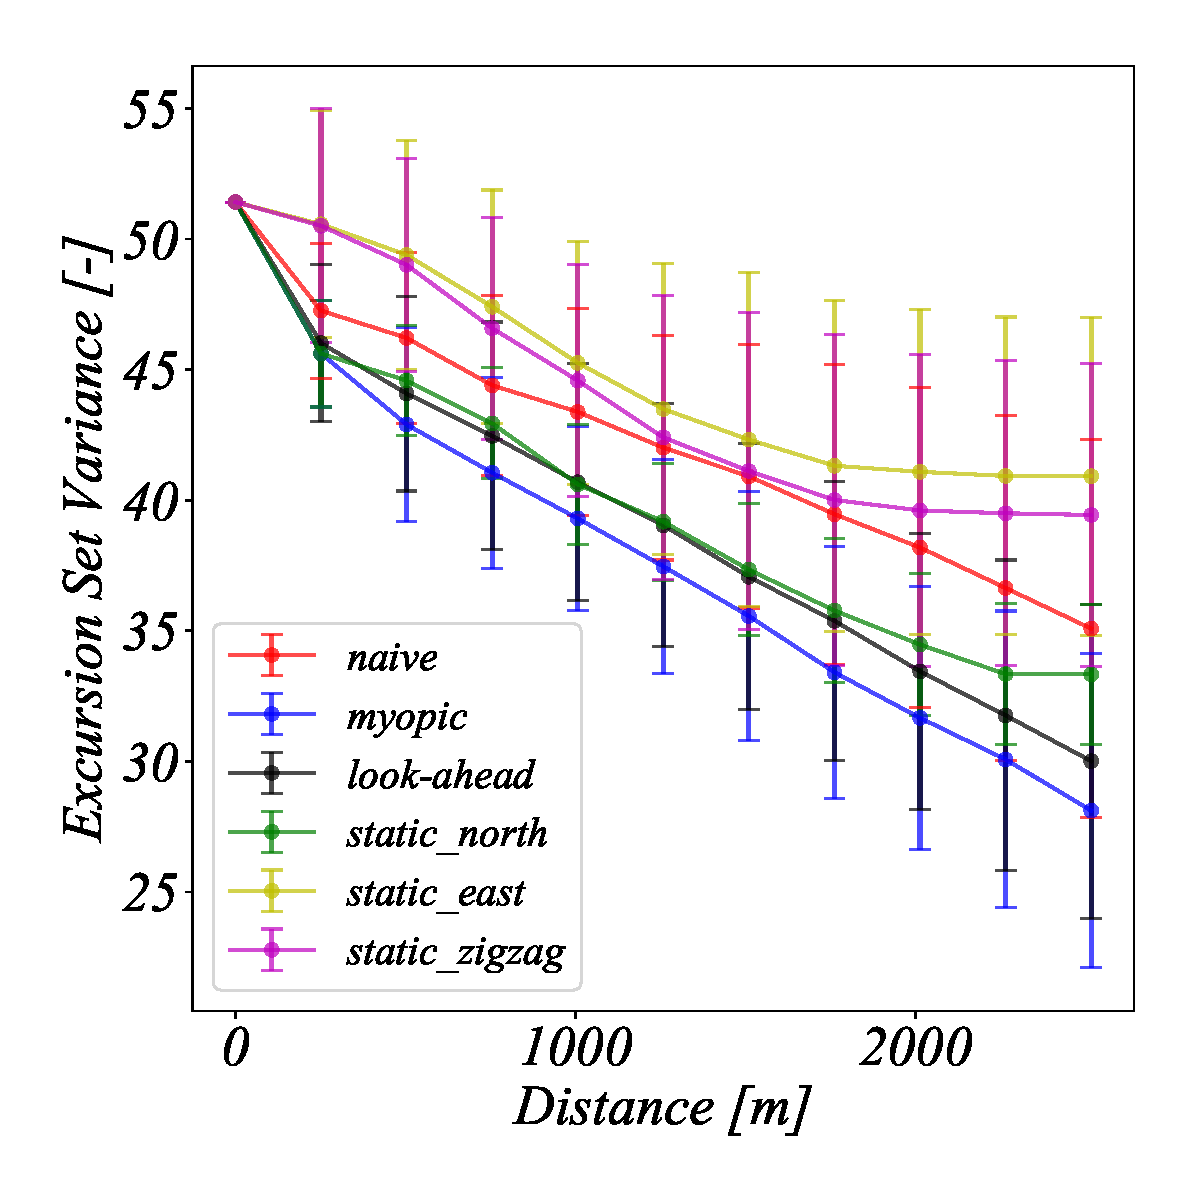
\includegraphics[height=0.49\textwidth]{Figures/sim/avg_EV.pdf}}
  \hfill
  \subfigure[RMSE between estimated field and truth.]{\label{fig:avg_rmse}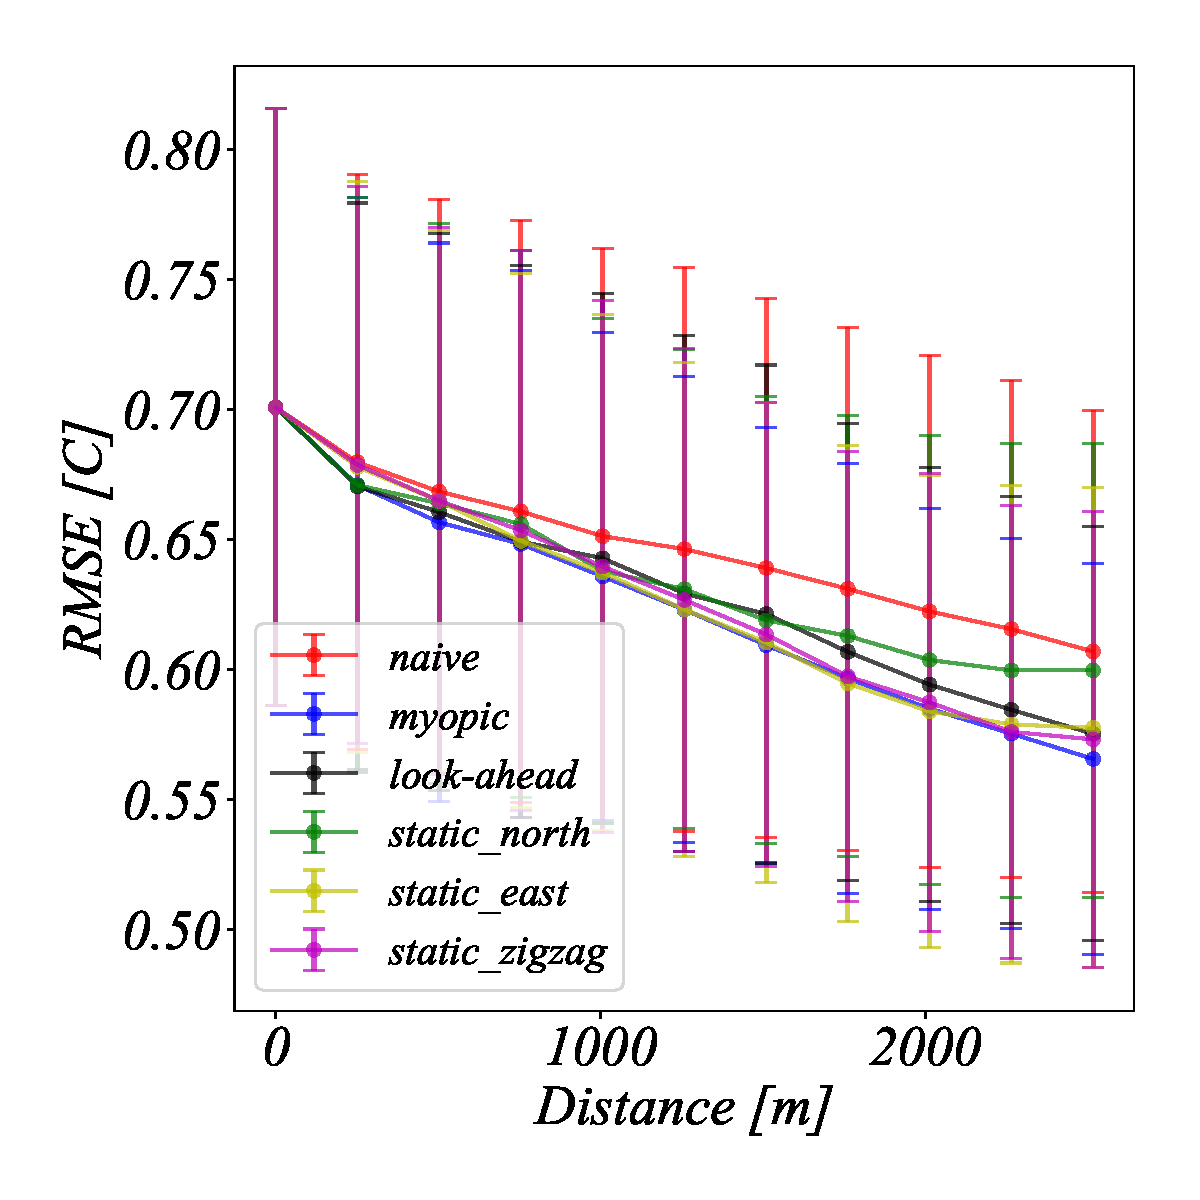
\includegraphics[height=0.49\textwidth]{Figures/sim/avg_RMSE.pdf}}
  \hfill 
  \subfigure[Explained variance $\bR^{2}$.]{\label{fig:avg_r2}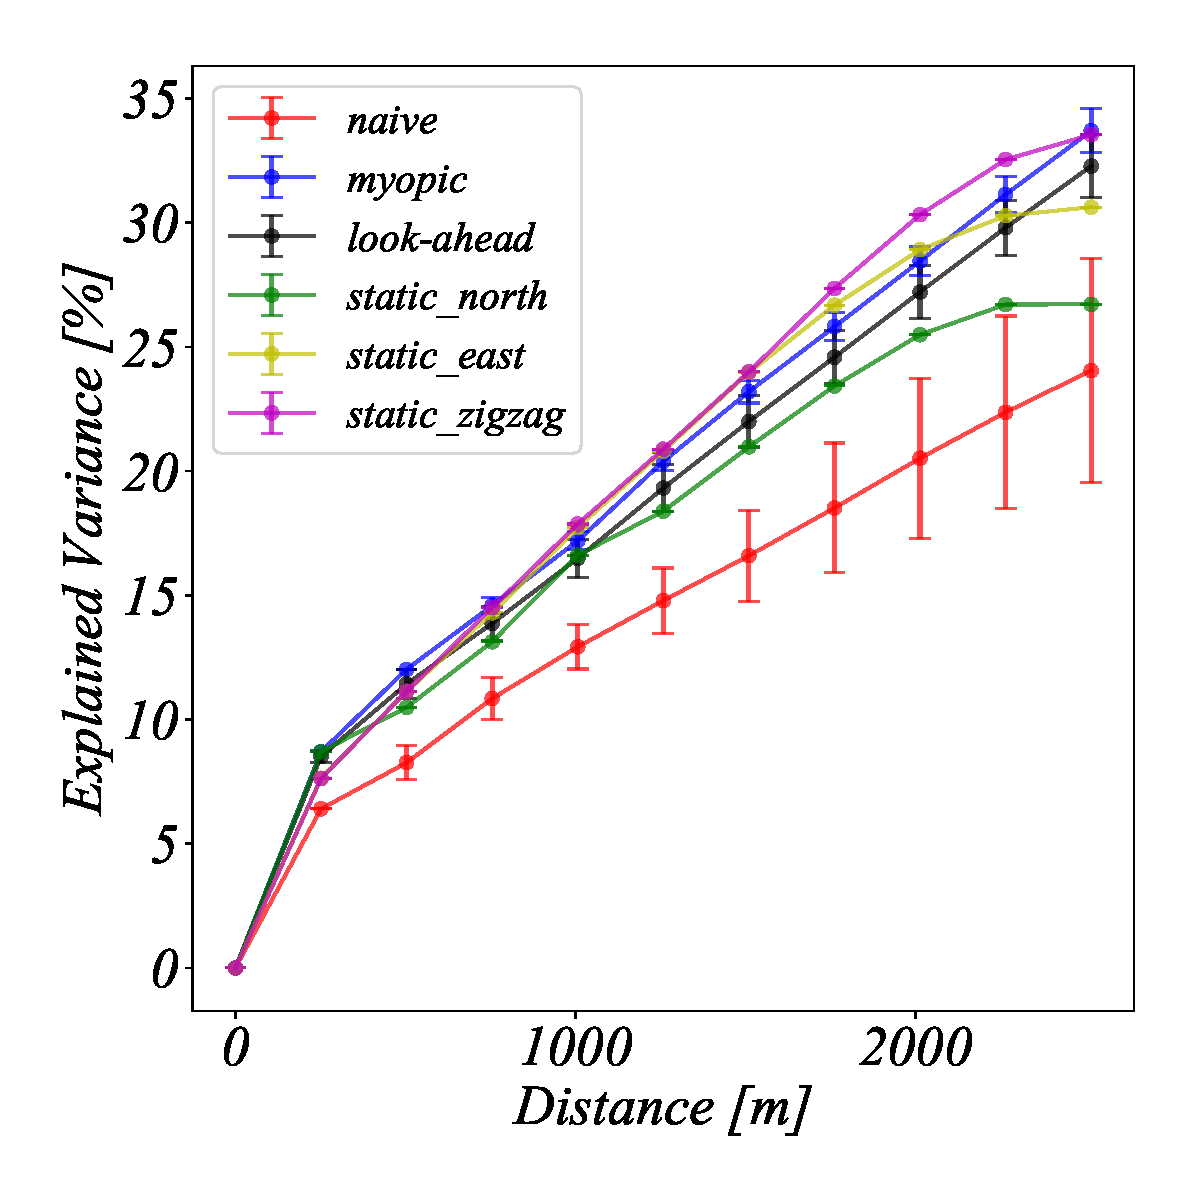
\includegraphics[height=0.49\textwidth]{Figures/sim/avg_R2.pdf}}
  \hfill 
  \subfigure[Time used to do inference.]{\label{fig:avg_time}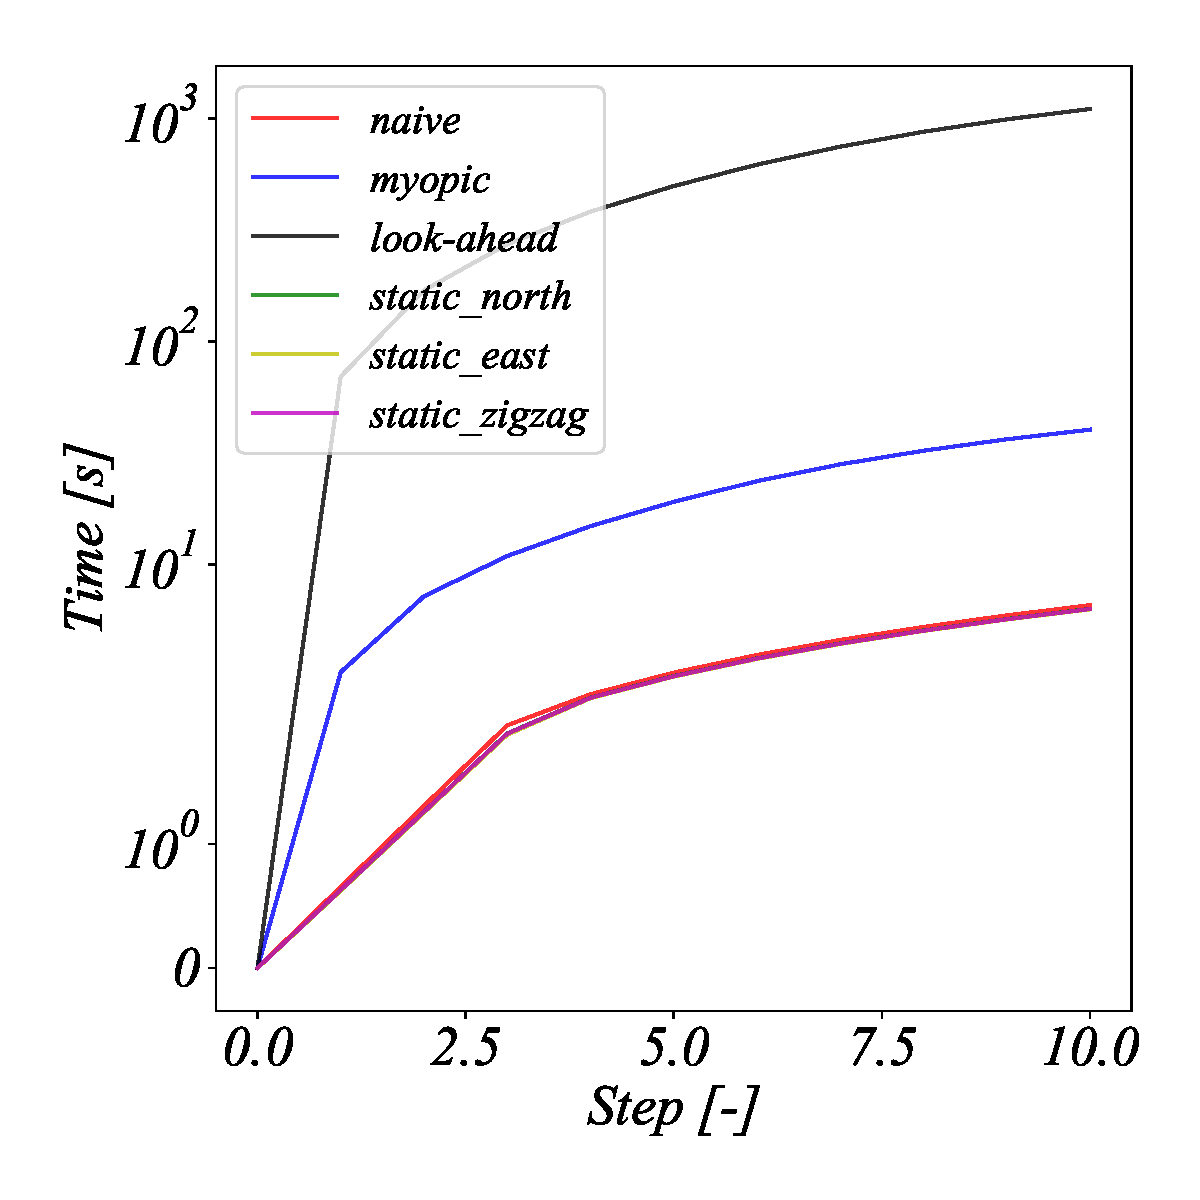
\includegraphics[height=0.49\textwidth]{Figures/sim/avg_Time.pdf}}
\caption{Simulation results from 100 replicate simulations for 10
  sampling choices/steps on the grid. (Updated:01.05.2019)} 
\label{fig:sim_results}
\end{figure}

Figure \ref{fig:avg_rmse} and \ref{fig:avg_r2} show the resulting drop in RMSE and increase in explained variance. Both \texttt{myopic} and \texttt{look-ahead} perform well here, but some of the \texttt{static\_east} and \texttt{static\_zigzag} also achieve good results because they are pre-determined to cover large parts of the domain without re-visitation. Sequential strategies targeting ES variance will sometimes not reach similar coverage as interesting data may draw the path into turns and twists that may result in re-visitation. 

\begin{figure}[!b]
  \centering
  \subfigure[Look-ahead]{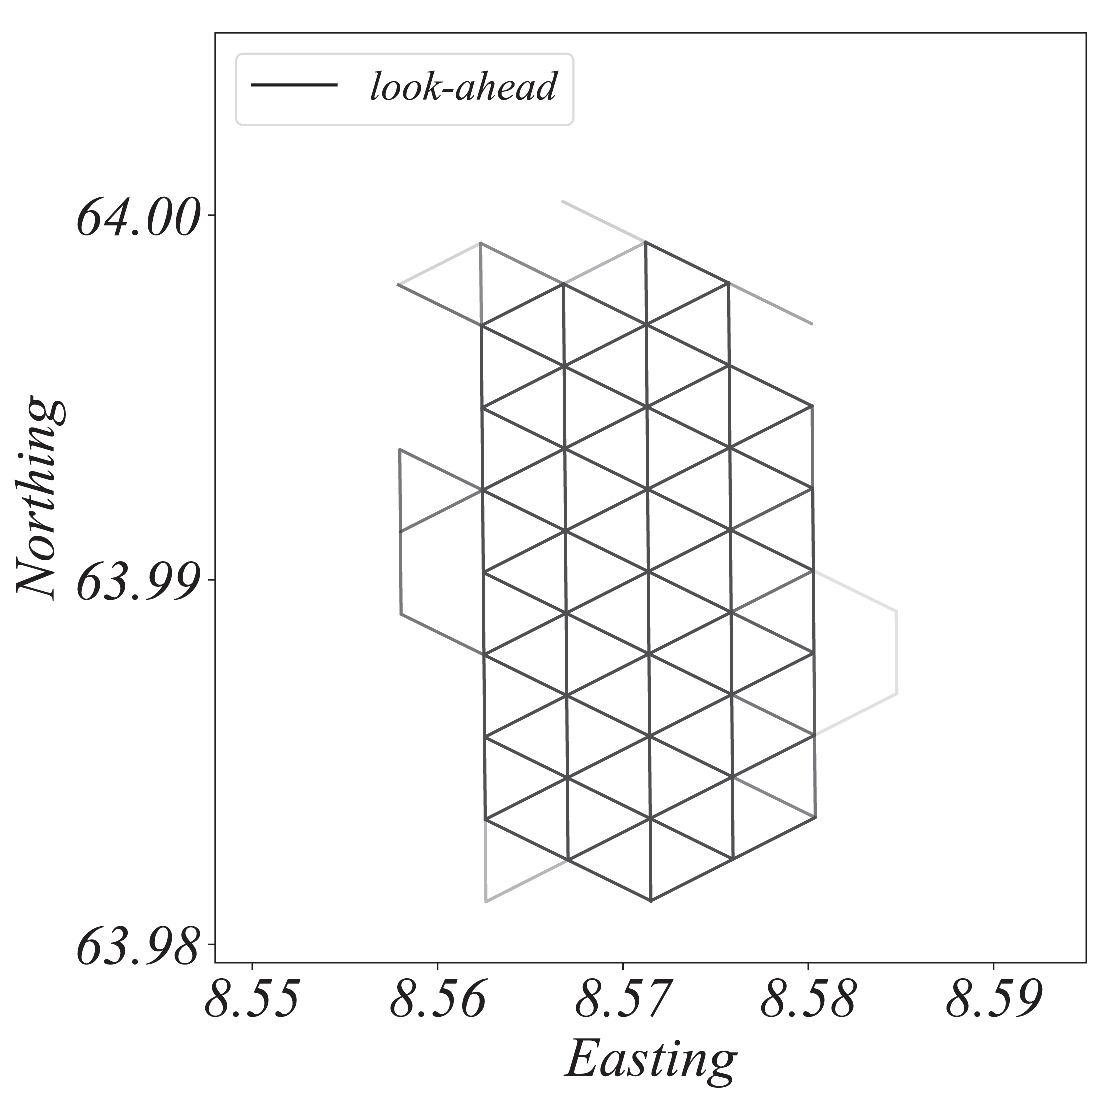
\includegraphics[height = 0.46\textwidth]{Figures/sim/route_look-ahead.pdf}\label{fig:avg_look-ahead}}
  \hfill
  \subfigure[Myopic]{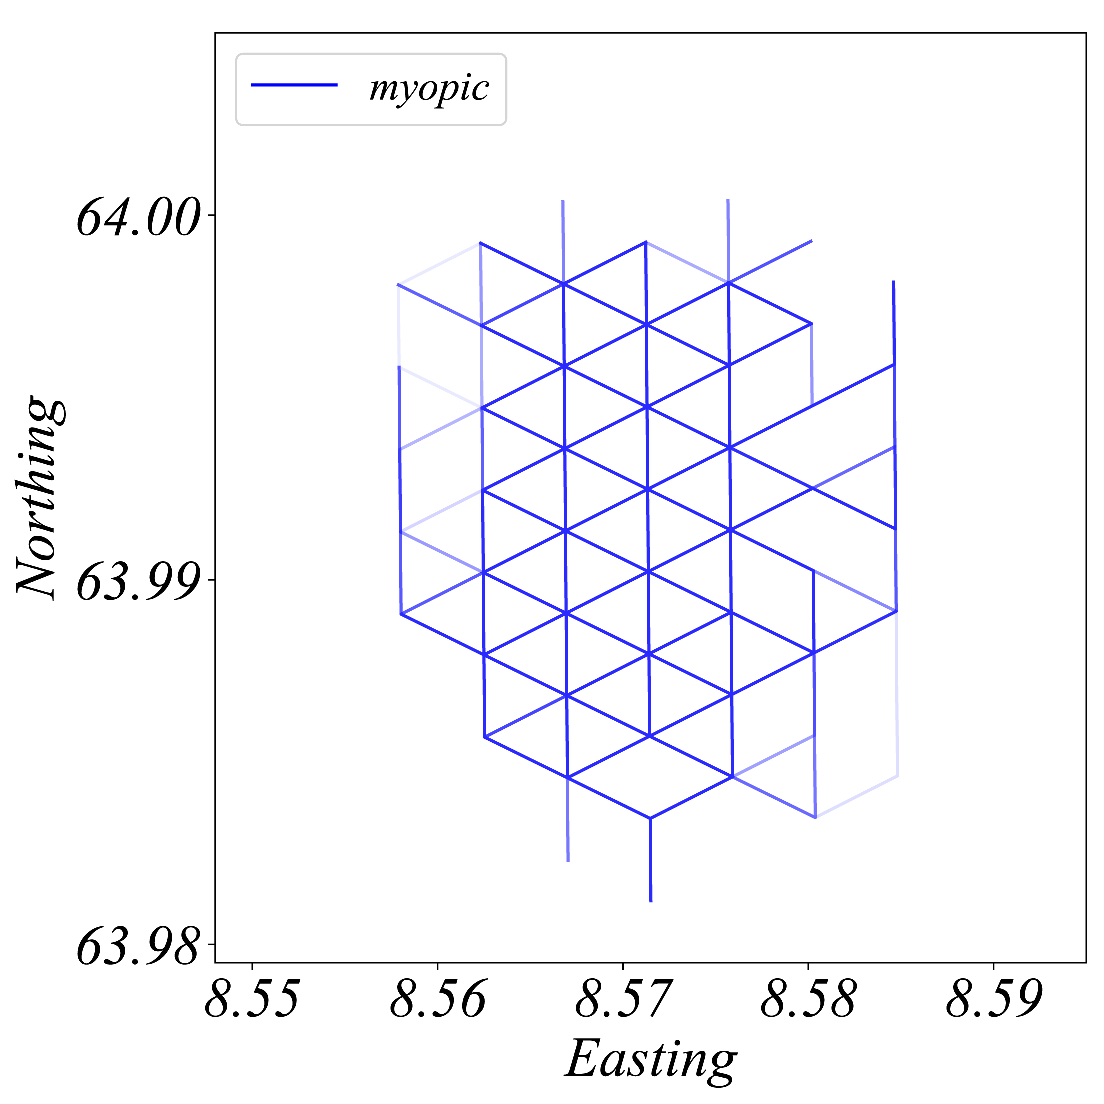
\includegraphics[height = 0.46\textwidth]{Figures/sim/route_myopic.pdf}\label{fig:avg_myopic}}
  \hfill
  \subfigure[Naive]{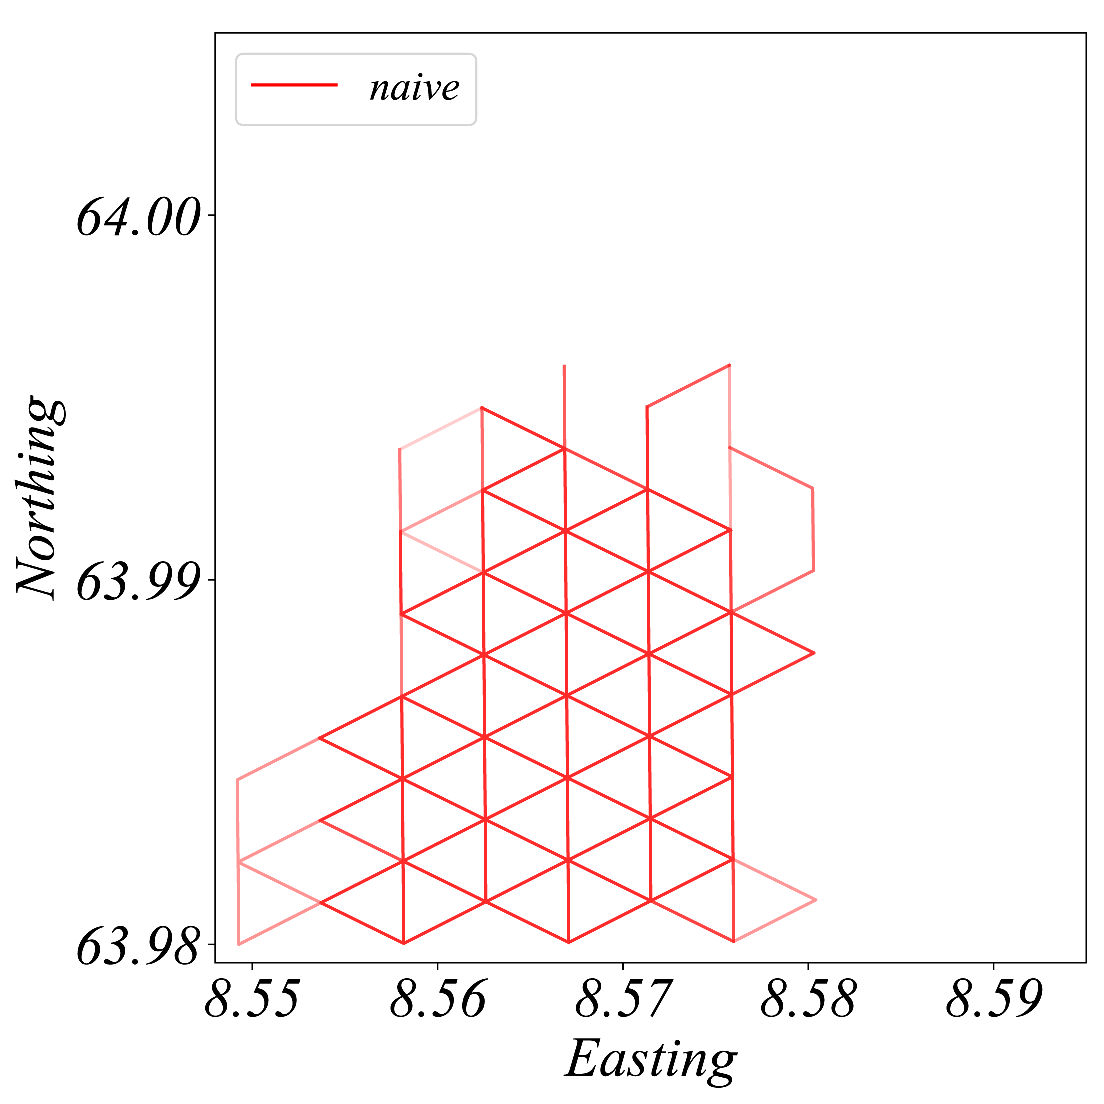
\includegraphics[height = 0.46\textwidth]{Figures/sim/route_naive.pdf}\label{fig:route_naive}}
  \hfill
  \subfigure[Static]{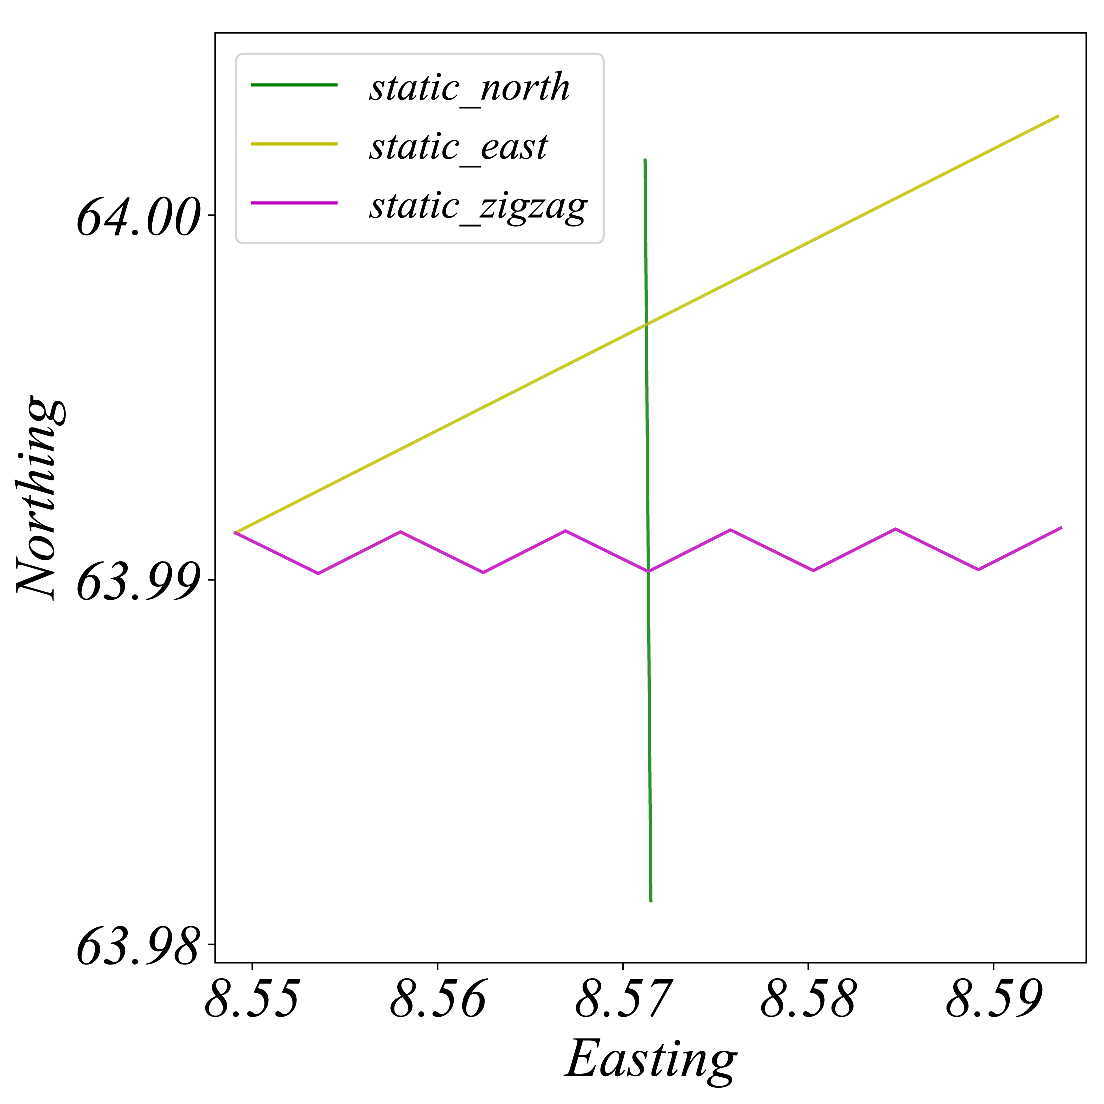
\includegraphics[height = 0.46\textwidth]{Figures/sim/route_static.pdf}\label{fig:route_static}}
  \hfill
  \caption{The overlaid route choices (strategies), superimposed for
    the 100 replicate surveys with 10 sampling choices/steps.}
\label{fig:route_choices}
\end{figure}

Fig.  \ref{fig:avg_time} shows the computational effort; the \texttt{naive} strategy is on par with the static designs, while the \texttt{myopic} strategy is slower and \texttt{look-ahead} more so, with the latter reaching levels that are nearly impractical for execution on a vehicle. Some pruning of the graph is performed to improve the computational speed, such as ruling out repeated visitations and back-and-forth routes. Some of the intermediate results are also stored for longer planning horizons. Still, more pruning of branches or inclusion of other heuristics could be included to make the strategy faster. Then again, the inclusion of heuristics is likely a contributing factor that the \texttt{look-ahead} strategy is not outperforming the \texttt{myopic} strategy. In Figure \ref{fig:route_choices} the realized sampling paths for each sequential schemes and static designs is shown.  

The \texttt{naive} strategy gets stuck in the southern part of the domain in some cases, because it is too focused on the probabilities near $0.5$. The \texttt{myopic} strategy meanwhile, covers a wider domain than the look-ahead, there are several reasons for this. First, a greedy approach will tend to do more put more emphasis on locations close to the agent, which may lead away from the centre. Secondly, as the agent evaluates the impact of locations further away (look-ahead) where assimilated data has less effect, the prior (which is centered here) will act to restrict paths deviating from the central zone.   

We further go on to study sensitivity of the result to different prior correlation values between temperature and salinity, prior standard deviations, spatial correlations, as well as measuring only temperature on-board the AUV (as indicated in the rows). We only compare results at the end of each survey. The expected ES variances are shown in Table \ref{tab:sim_res_ev}, results of RMSE are in Table \ref{tab:sim_res_rmse}, and explained variance in Table \ref{tab:sim_res_r2}. In all runs, both the \texttt{myopic} and \texttt{look-ahead} strategies perform the best in terms of expected variance in the ES. Surprisingly, the \texttt{myopic} is on-par and even slightly better than the \texttt{look-ahead} strategy. Part of the reason can be traced to the act of pruning some of the paths for the \texttt{look-ahead} strategy, but even with less pruning, the \texttt{look-ahead} does not outperform the \texttt{myopic} approach. The \texttt{static\_north} design is clearly better than the other two static designs, the reason being that the others do not focus on the areas where the ES is really uncertain (centre locations are the most uncertain). By measuring temperature alone the expected variances in the ES is only slightly higher. This occurs because the ES is almost the same and because of the correlation of $0.6$, which means that temperature observations provide information about salinity as well. For the other predictive measures, \texttt{myopic} and \texttt{look-ahead} do well, clearly beating the \texttt{naive} strategy. The \texttt{static\_zigzag} design is usually the best among the static designs for these predictive performance measures because its pattern gives more effective coverage of the domain when there is significant spatial correlation as in this case.

\begin{table}[!h]
    \centering
    \scalebox{0.87}{
    \begin{tabular}{lrrrrrr}
    \toprule
    Parameter: $E_{\by}(p[1-p])$ &  naive &  myopic &  look-ahead &  static\_north &  static\_east &  static\_zigzag \\
    \midrule
                    \rowcolor{Gray}
ts. cor. low: 0.2  &  29.65 &   27.08 &       \textbf{26.44} &         32.33 &        40.31 &          36.23 \\
ts. cor. high: 0.8 &  36.18 &   \textbf{28.42} &       30.30 &         32.99 &        37.18 &          36.04 \\
                    \rowcolor{Gray}
std. low: 0.1      &  18.26 &   15.79 &       \textbf{15.35} &         18.89 &        26.65 &          26.10 \\
std. high: 0.5     &  47.01 &   \textbf{41.31} &       43.15 &         47.92 &        52.63 &          49.71 \\
                    \rowcolor{Gray}
cor. low: 0.8      &  44.42 &   \textbf{42.02} &       42.47 &         43.84 &        46.05 &          47.82 \\
cor. high: 0.2     &  29.73 &   21.09 &       \textbf{20.43} &         27.91 &        37.60 &          34.35 \\
                    \rowcolor{Gray}
temp. only         &  38.25 &   29.16 &       \textbf{28.69} &         34.32 &        39.81 &          36.17 \\
basecase           &  35.21 &   \textbf{28.56} &       28.94 &         33.50 &        39.84 &          39.26 \\
    \bottomrule
    \end{tabular}}
  \caption{Simulation results for the final mean IBV (Eq. \eqref{two_partsK}).}
    \label{tab:sim_res_ev}
\end{table}
\vspace{-0.4cm}
\begin{table}[!h]
    \centering
    \scalebox{0.92}{
        \begin{tabular}{lrrrrrr}
        \toprule
        Parameter: RMSE &  naive &  myopic &  look-ahead &  static\_north &  static\_east &  static\_zigzag \\
        \midrule
                \rowcolor{Gray}
ts. cor. low: 0.2  &   0.63 &    \textbf{0.57} &        0.59 &          0.62 &         0.57 &           0.59 \\
ts. cor. high: 0.8 &   0.63 &    \textbf{0.59} &        0.61 &          0.64 &         0.60 &           0.60 \\
                \rowcolor{Gray}
std. low: 0.1      &   0.39 &    0.37 &        0.38 &          0.38 &         0.40 &           \textbf{0.35} \\
std. high: 0.5     &   0.85 &    0.82 &        0.84 &          0.82 &         0.83 &           \textbf{0.81} \\  
                \rowcolor{Gray}
cor. low: 0.8      &   0.68 &    0.66 &        0.67 &          0.68 &         0.66 &           \textbf{0.65} \\
cor. high: 0.2     &   0.58 &    0.54 &        0.55 &          0.58 &         0.54 &           \textbf{0.49} \\
                \rowcolor{Gray}
temp. only         &   0.65 &    0.63 &        0.62 &          0.65 &         \textbf{0.61} &           0.62 \\
basecase           &  0.61 &   \textbf{0.56} &       \textbf{0.56} &         0.60 &        0.57 &          0.57 \\
        \bottomrule
        \end{tabular}}
      \caption{Simulation results for the final mean RMSE ($\frac{1}{B} \sum_{b=1}^{B} \sqrt{(\bmu-\tilde{\bmu})^2}$).}
    \label{tab:sim_res_rmse}
\end{table}
\vspace{-0.4cm}
\begin{table}[!h]
    \centering
    \scalebox{0.95}{
        \begin{tabular}{lrrrrrr}
        \toprule
        Parameter: $\bR^{2}$ &  naive &  myopic &  look-ahead &  static\_north &  static\_east &  static\_zigzag \\
        \midrule
                        \rowcolor{Gray}
ts. cor. low: 0.2  &  27.00 &   33.29 &       32.24 &         26.71 &        30.56 &          \textbf{33.50} \\
ts. cor. high: 0.8 &  23.68 &   \textbf{33.87} &       32.42 &         26.72 &        30.73 &          33.61 \\
                        \rowcolor{Gray}
std. low: 0.1      &  25.38 &   30.80 &       30.29 &         26.09 &        28.75 &          \textbf{31.66} \\
std. high: 0.5     &  26.11 &   34.22 &       32.48 &         26.95 &        31.77 &          \textbf{34.48} \\
                        \rowcolor{Gray}
cor. low: 0.8      &   8.80 &   11.50 &       11.23 &          9.56 &        12.31 &          \textbf{12.58} \\
cor. high: 0.2     &  37.57 &   \textbf{48.68} &       48.11 &         39.61 &        41.98 &          48.04 \\
                        \rowcolor{Gray}
temp. only         &  11.67 &   \textbf{22.82} &       21.98 &         18.16 &        20.77 &          22.78 \\
basecase           &  24.71 &   33.45 &       32.25 &         26.71 &        30.62 &          \textbf{33.54}\\
        \bottomrule
        \end{tabular}}
      \caption{Simulation results for the final mean explained variance $\bR^{2}=100*(1-(\bSigma_{posterior}/\bSigma_{initial}))$).}
    \label{tab:sim_res_r2}
\end{table}

\newpage

\section{Case study - Mapping a river plume}
\label{sec:case_study}

To demonstrate the applicability of using multivariate EPs and the IBV to inform oceanographic sampling, we present a case study mapping a river plume with an AUV. The experiment was performed in Trondheim, Norway,
surveying the Nidelva river (Figure \ref{fig:nidelven}). Here cold and fresh water from the river meet the warm and saline ocean water in the Trondheim fjord. The experiment is focused along the eastern shoreline due to the aforementioned Coriolis force. The frontal zone therefore runs more or less parallel to the eastern shore as
indicated in purple in Figure \ref{fig:nidelven}. The experiments were conducted in late Spring 2019, when there is still snow melting in the surrounding mountains so that the river water is substantially colder than the water in the fjord.

\subsection{Model specification}

The statistical model parameters were specified based on a short preliminary survey where the AUV did an initial transect to determine the environmental conditions and correlation structure. Based on the initial data the trend parameters were estimated by linear regression, where both temperature and salinity are assumed to increase linearly, going west from the river mouth. Next, the residuals from the regression analysis are analyzed to study the fit of the Gaussian model and to specify the covariance parameters.

\begin{figure}[!h] 
 \centering 
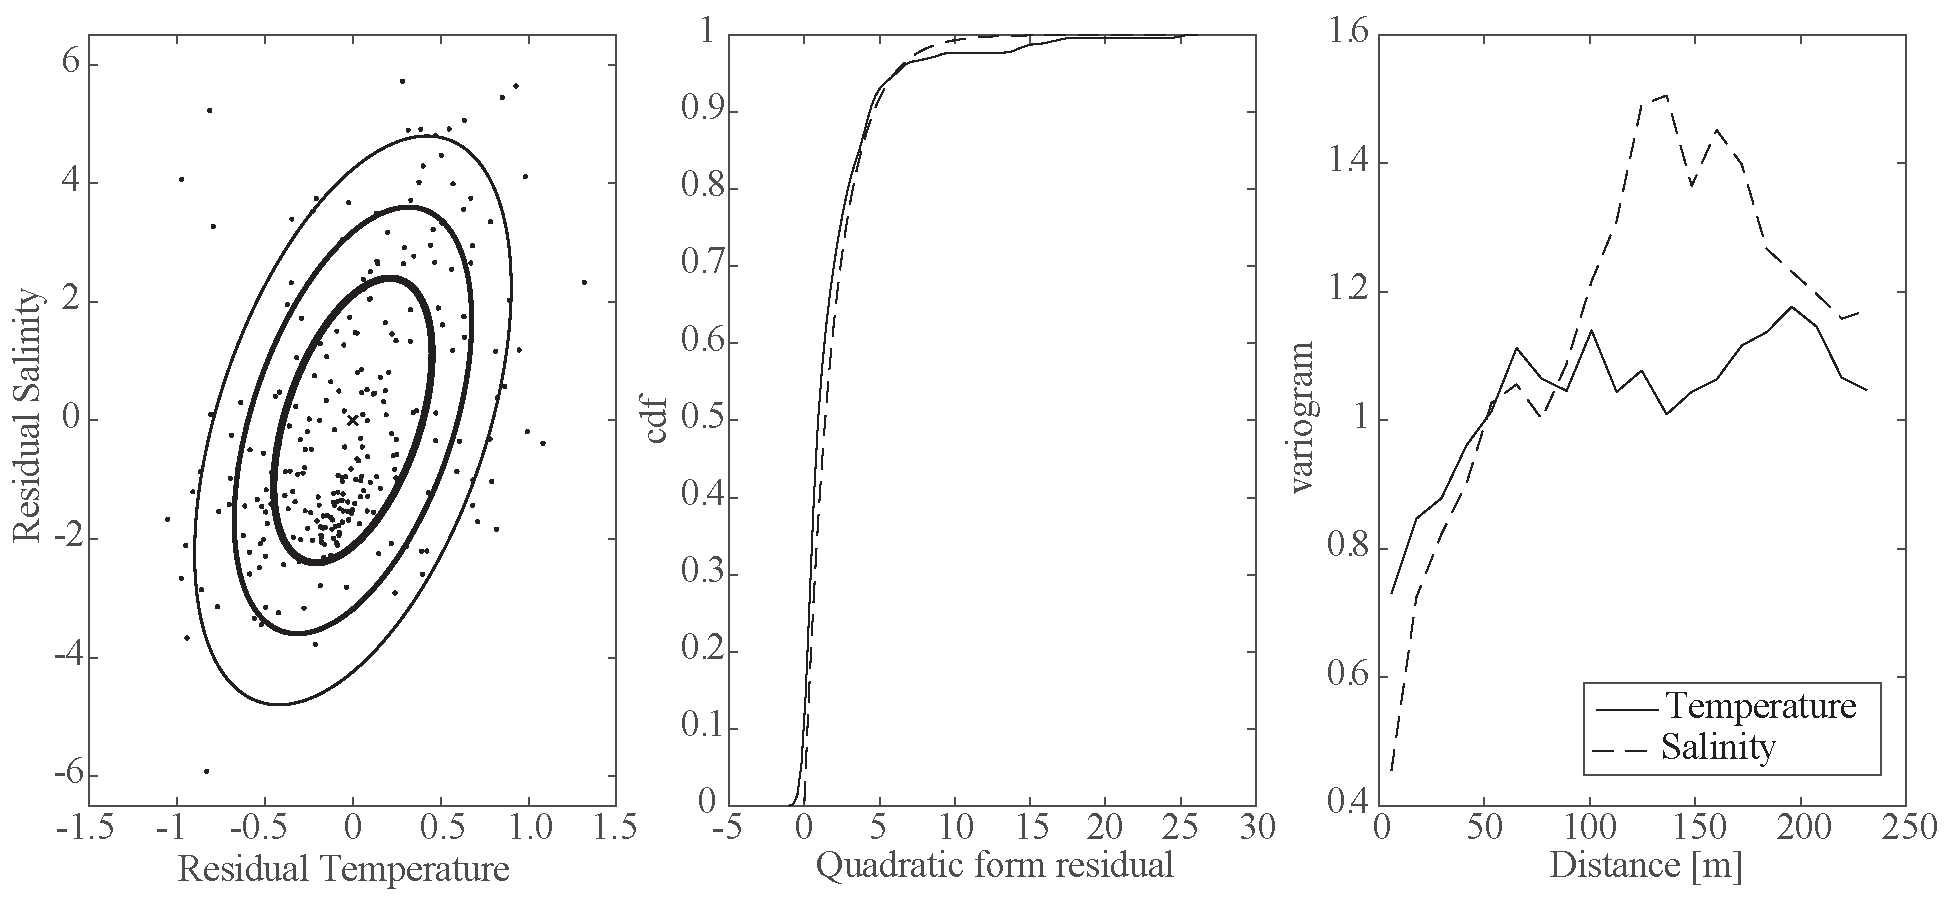
\includegraphics[width=0.98\textwidth]{Figures/field-trials/res_diag.pdf}
\caption{Data analysis from a preliminary trial experiment using the
  AUV. Left: Residual plot of temperature and salinity along with
  Gaussian contours. Middle: Empirical CDF of the quadratic form of
  the residuals along with the theoretical CDF of the $\chi^2$
  distribution with two degrees of freedom. Right: Empirical variogram
  of the salinity and temperature data.} \label{fig:parest}
\end{figure}

Figure \ref{fig:parest} shows diagnostic plots of this analysis. The display on the left shows a cross-plot of temperature and salinity residuals, after the westernly trends in both salinity and temperature are subtracted from the data. This scatterplot of joint residuals indicates larger variability in salinity than in temperature, and a positive correlation ($0.5$) between the two variables. Based on the fitted bivariate Gaussian model (ellipses in left display), we can compute the modeled quadratic form of the residuals, and if the model is adequate they should be approximately $\chi^2_2$ distributed. Figure \ref{fig:parest} (middle) shows the empirical (cumulative distribution function) CDF of these quadratic forms (solid) together with the theoretical CDF of the $\chi^2_2$ distribution. The modeled and theoretical curves are very similar and this indicates that the Gaussian model fits reasonable well. Even though there appears to be some clustering in both left and middle displays of Figure \ref{fig:parest}, the bivariate diagnostic plots look reasonable and justify a Gaussian model. Figure \ref{fig:parest} (right) shows the empirical variogram of the scaled residuals for temperature and salinity. The decay is similar for the two, and seems to be negligible after about $150$ m. 


Based on the analysis in Fig. \ref{fig:parest} the resulting parameters are given in Table \ref{tab:experiment_param}. The regression parameters shown here are scaled to represent the east and west boundaries of the domain as seen in the preliminary transect data, and the thresholds are intermediate values. These parameter values were then used in field trials, where we explored the algorithm's ability to characterize the river plume front separating the river and fjord water masses, providing a spatial map of this boundary. 

%Mapping the spatial extent of a frontal zones is an important problem for studying many bio-physical interactions in the ocean. The frontal zone is determined by the boundary where plumes of sediments, nutrients, and possibly pollutants spreading from the river outlet meet and interact with adjacent coastal water. Due to the lower density the plumes spread on the surface, creating a front with an sharp gradient in both temperature and salinity. 

\begin{table}[!h]
\centering
\begin{tabular}{lrr}
\toprule
Parameter & Value & Source\\
\midrule
\rowcolor{Gray}
Cross correlation temp. and sal. & 0.5 & AUV observations\\
Temp. variance &  0.20 & AUV observations (variogram)\\
\rowcolor{Gray}
Sal. variance &  5.76 & AUV observations (variogram)\\
Corr. range  & 0.15 km & AUV observations (variogram)\\
\rowcolor{Gray}
River temp. $T_{river}$ & $10.0\,^{\circ}\mathrm{C}$ & AUV observations\\
Ocean temp. $T_{ocean}$ & $11.0\,^{\circ}\mathrm{C}$ & AUV observations\\
\rowcolor{Gray}
River sal. $S_{river}$ & $14.0$ g/kg & AUV observations\\
Ocean sal. $S_{ocean}$ & $22.0$ g/kg & AUV observations\\
\rowcolor{Gray}
Threshold temp. & $10.5\,^{\circ}\mathrm{C}$ & $(T_{ocean}-T_{river})/2+T_{river}$\\
Threshold sal. & $18.0$ g/kg & $(S_{ocean}-S_{river})/2+S_{river}$\\
\rowcolor{Gray}
\bottomrule
\end{tabular}
\caption{Model and threshold parameters found from an initial AUV
  survey. Observations were taken across the front while crossing from
  fresh cold river water to saline and warmer ocean waters.}
\label{tab:experiment_param}
\end{table}


\subsection{Experimental setup}

The sampling locations was distributed over an equilateral grid, as shown in Fig. \ref{fig:map} in a grey colored lattice. The robotic platform consisted of a Light AUV \citep{sousa2012lauv} (Figure \ref{fig:lauv}) equipped with a 16 Hz Seabird Fastcat-49 CTD (conductivity, temperature, and depth) sensor providing temperature and salinity measurements. The accuracy of the CTD instrument is $\pm 0.0003$ S/m (conductivity) and $\pm0.002\,^{\circ}\mathrm{C}$ (temperature). The sampling agent was built on top of the autonomous agent framework \texttt{T-REX} \citep{py10,Rajan12,Rajan12b}, running an instance of the \texttt{myopic} strategy from Section \ref{sec:sampling_designs}, to control the AUV and decide between sampling locations.

\begin{figure}[!h] 
\centering 

\includegraphics[width=0.98\textwidth]{Figures/harald.jpg}
\caption{The commercially available Light Autonomous Underwater Vehicle (LAUV) platform (Harald) for upper water-
column exploration used in the experiment.}
\label{fig:lauv}
\end{figure} 

The sampling strategy was designed around the concept of visiting waypoints sequentially. Arriving at a desired waypoint, with new measurements and an updated model, the AUV triggers the myopic strategy to evaluate all possible design criteria, e.g Eq. \eqref{critSEQ}. The waypoint-and-path combination which is expected to reduce the IBV the most is selected; upon arrival this procedure is then repeated. At each stage, it takes the AUV about 30 sec to evaluate the expected IBV for all the possible waypoint-and-path alternatives.

The AUV was set to start in the south center part of the waypoint graph, with the previously outlined GP prior model of the environment. Each AUV survey was set to take approximately 40 min, visiting 15 waypoints on the grid, with the AUV running near the surface to better capture the plume. On its path from one waypoint to the next, the AUV gathered data regularly, and the GP model assimilated temperature and salinity data with an update frequency of 30 sec, about three updates per stage.

\begin{figure*}[!h]
\centering
\subfigure[Survey map.]{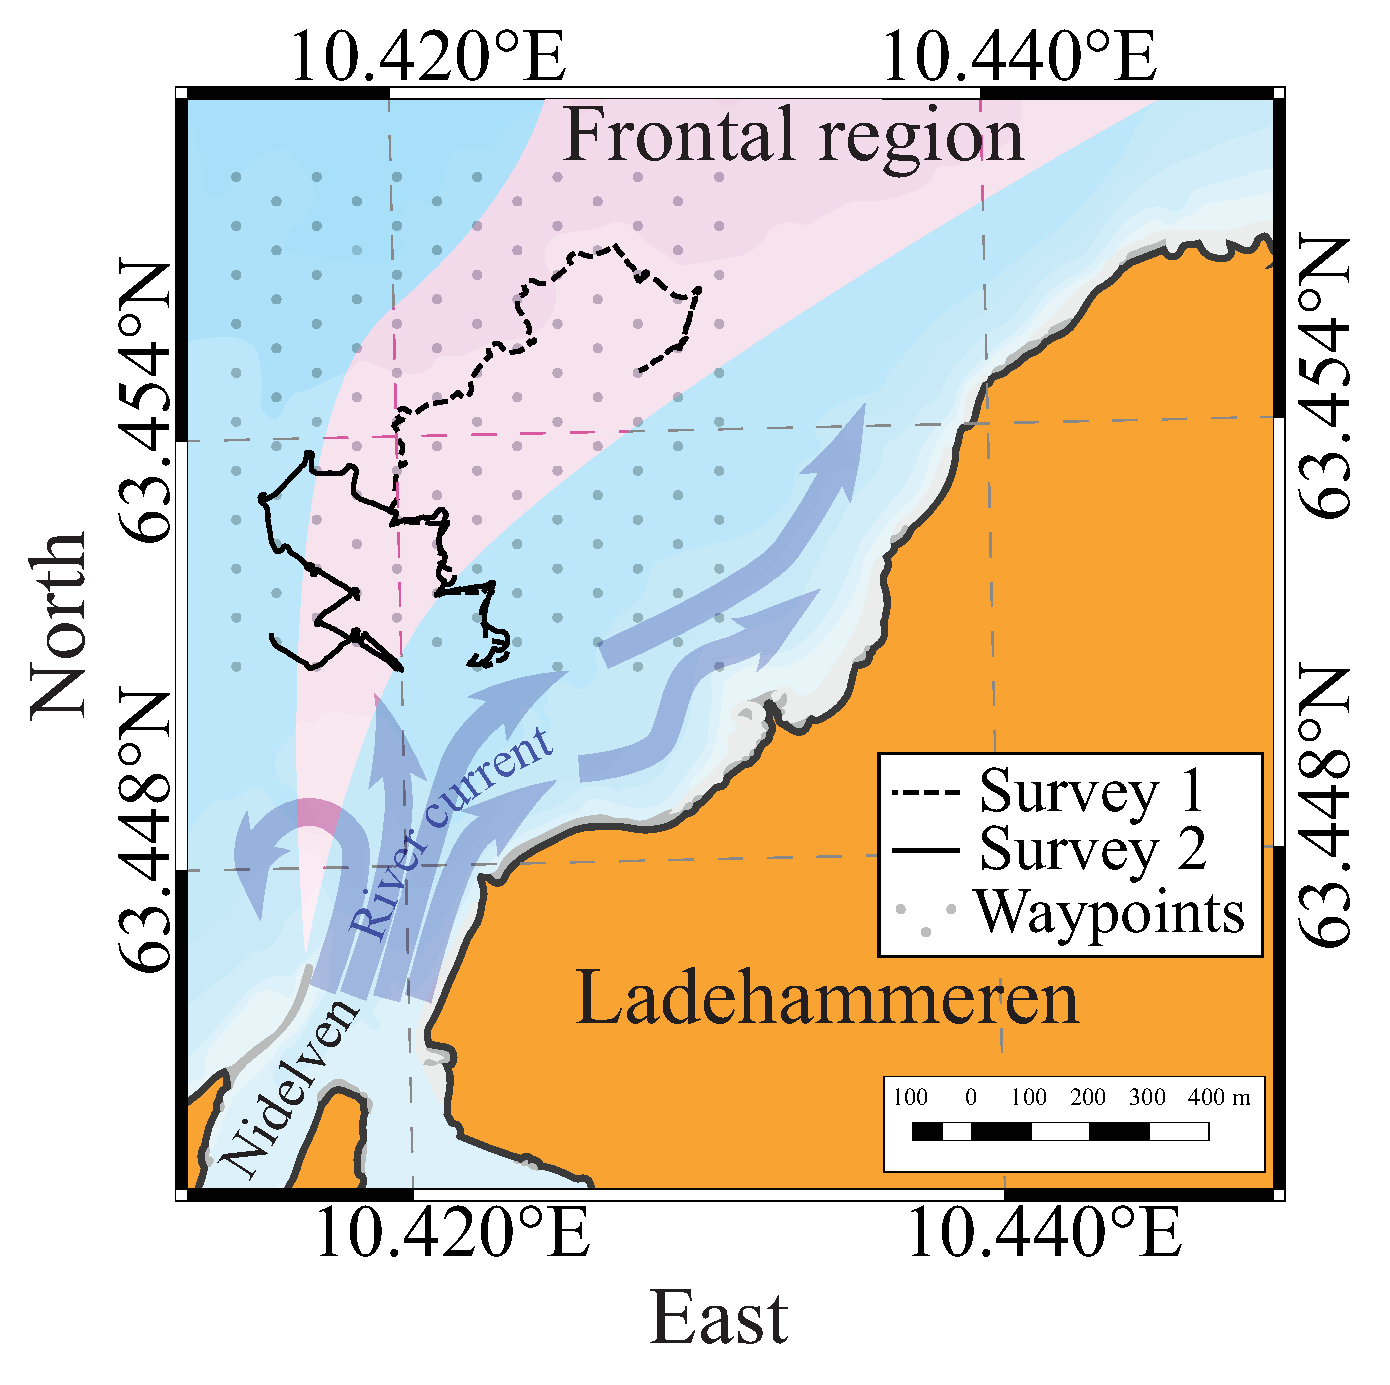
\includegraphics[height=0.41\textwidth]{Figures/field-trials/alt_map.eps}\label{fig:map}}
\hspace{0.3cm}
\subfigure[Temperature tracks.]{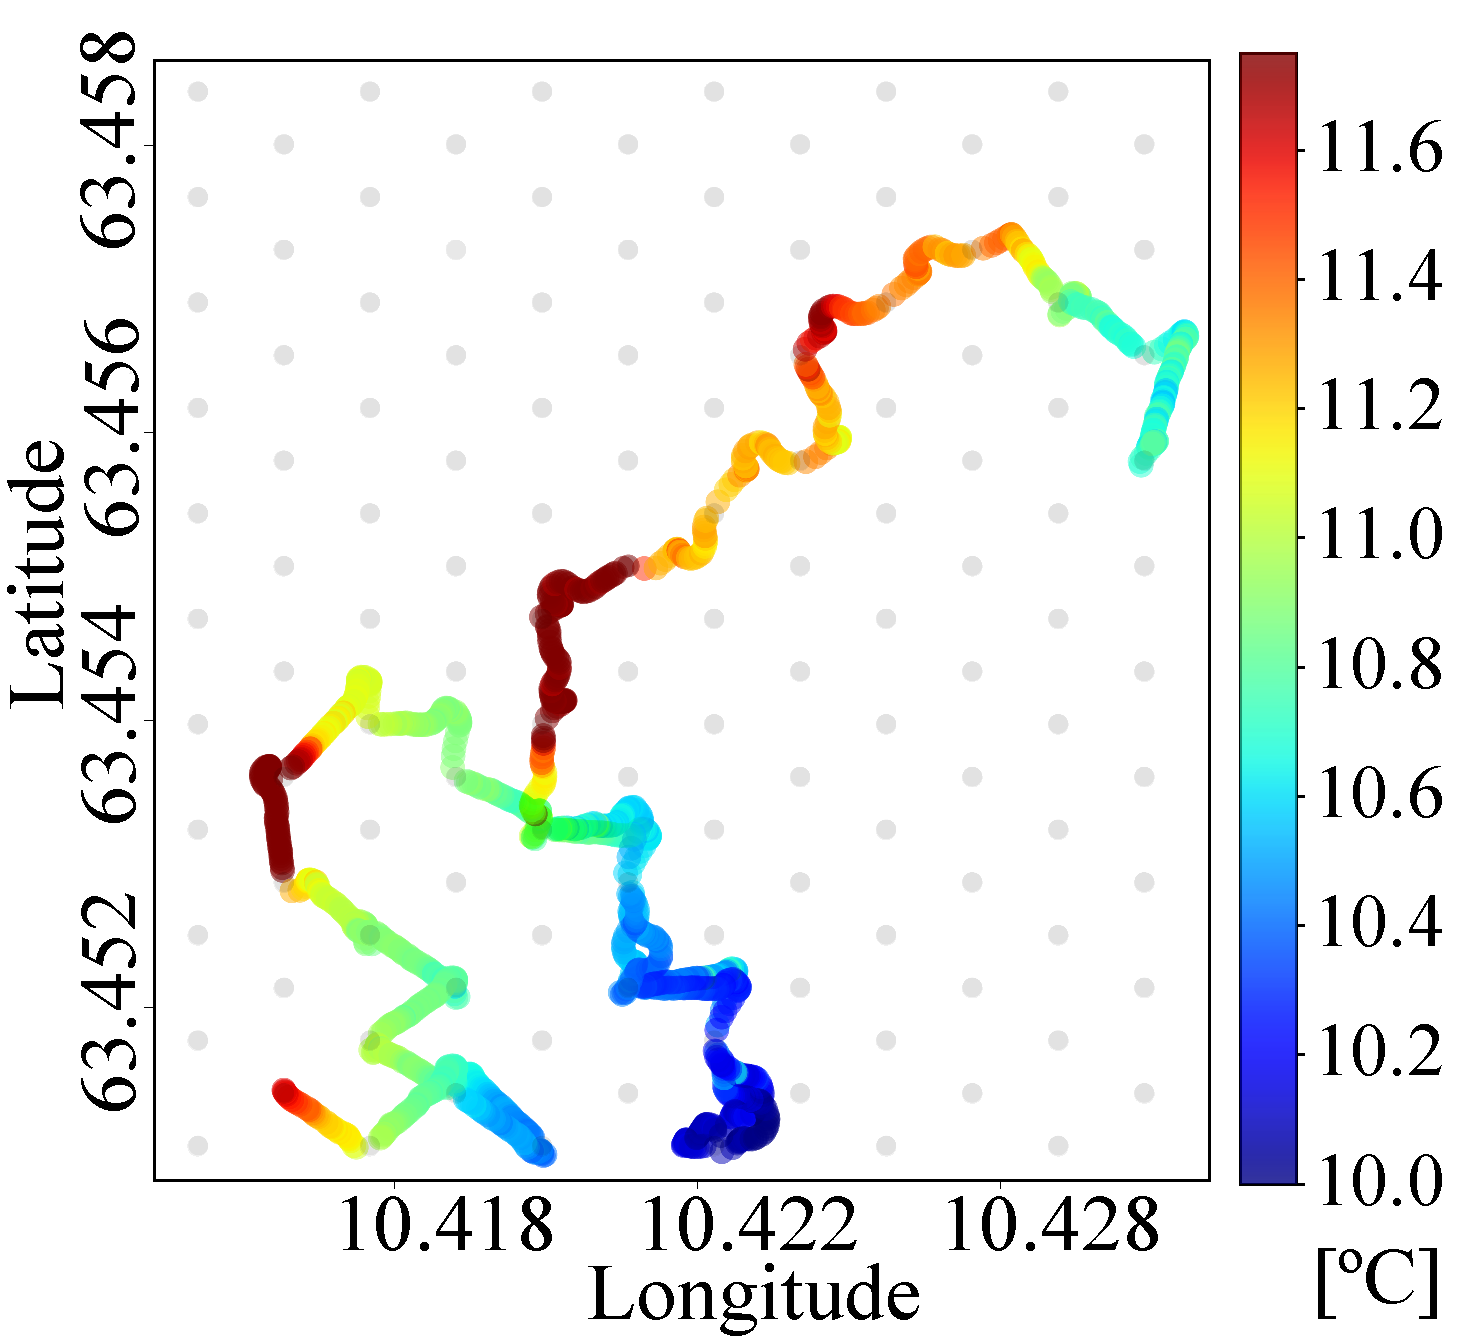
\includegraphics[height=0.41\textwidth]{Figures/field-trials/auv.pdf}\label{fig:res_both}}

\subfigure[Survey 1]{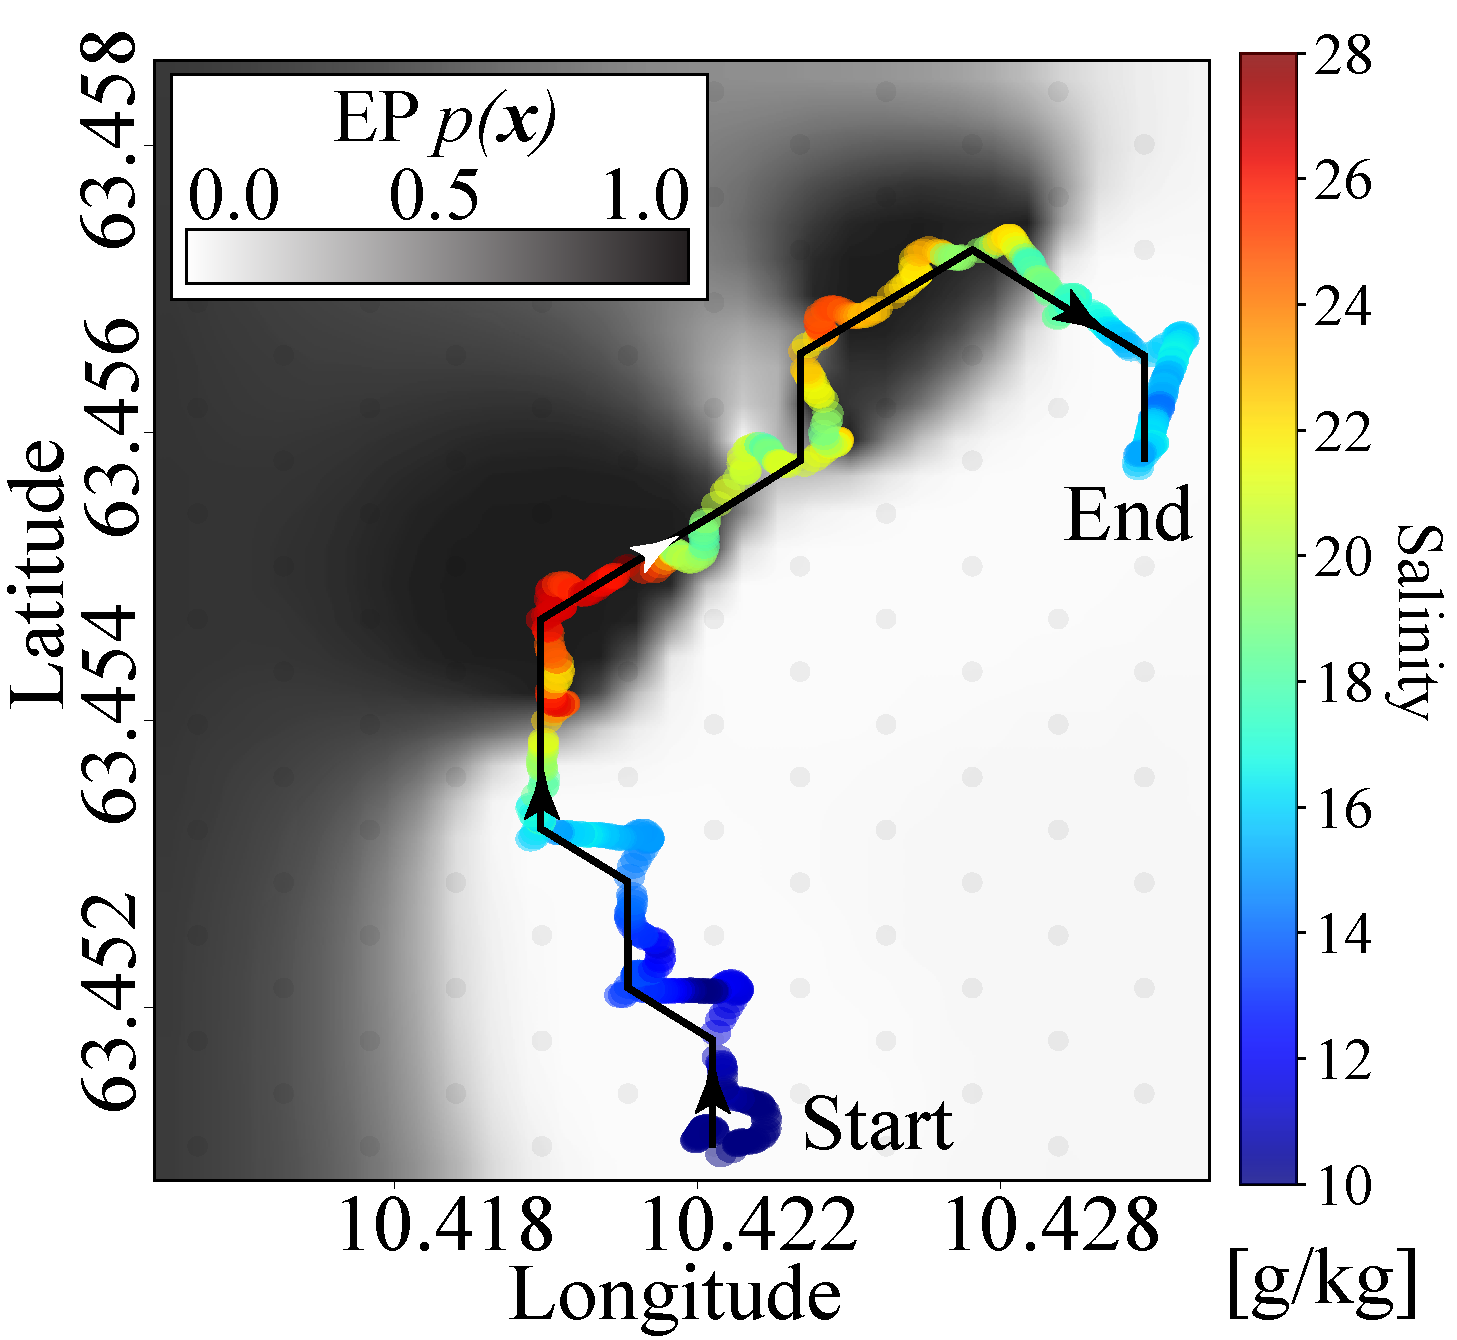
\includegraphics[height=0.40\textwidth]{Figures/field-trials/auv1_es_sal.pdf}\label{fig:res1}}
\hspace{0.2cm}
\subfigure[Survey 2]{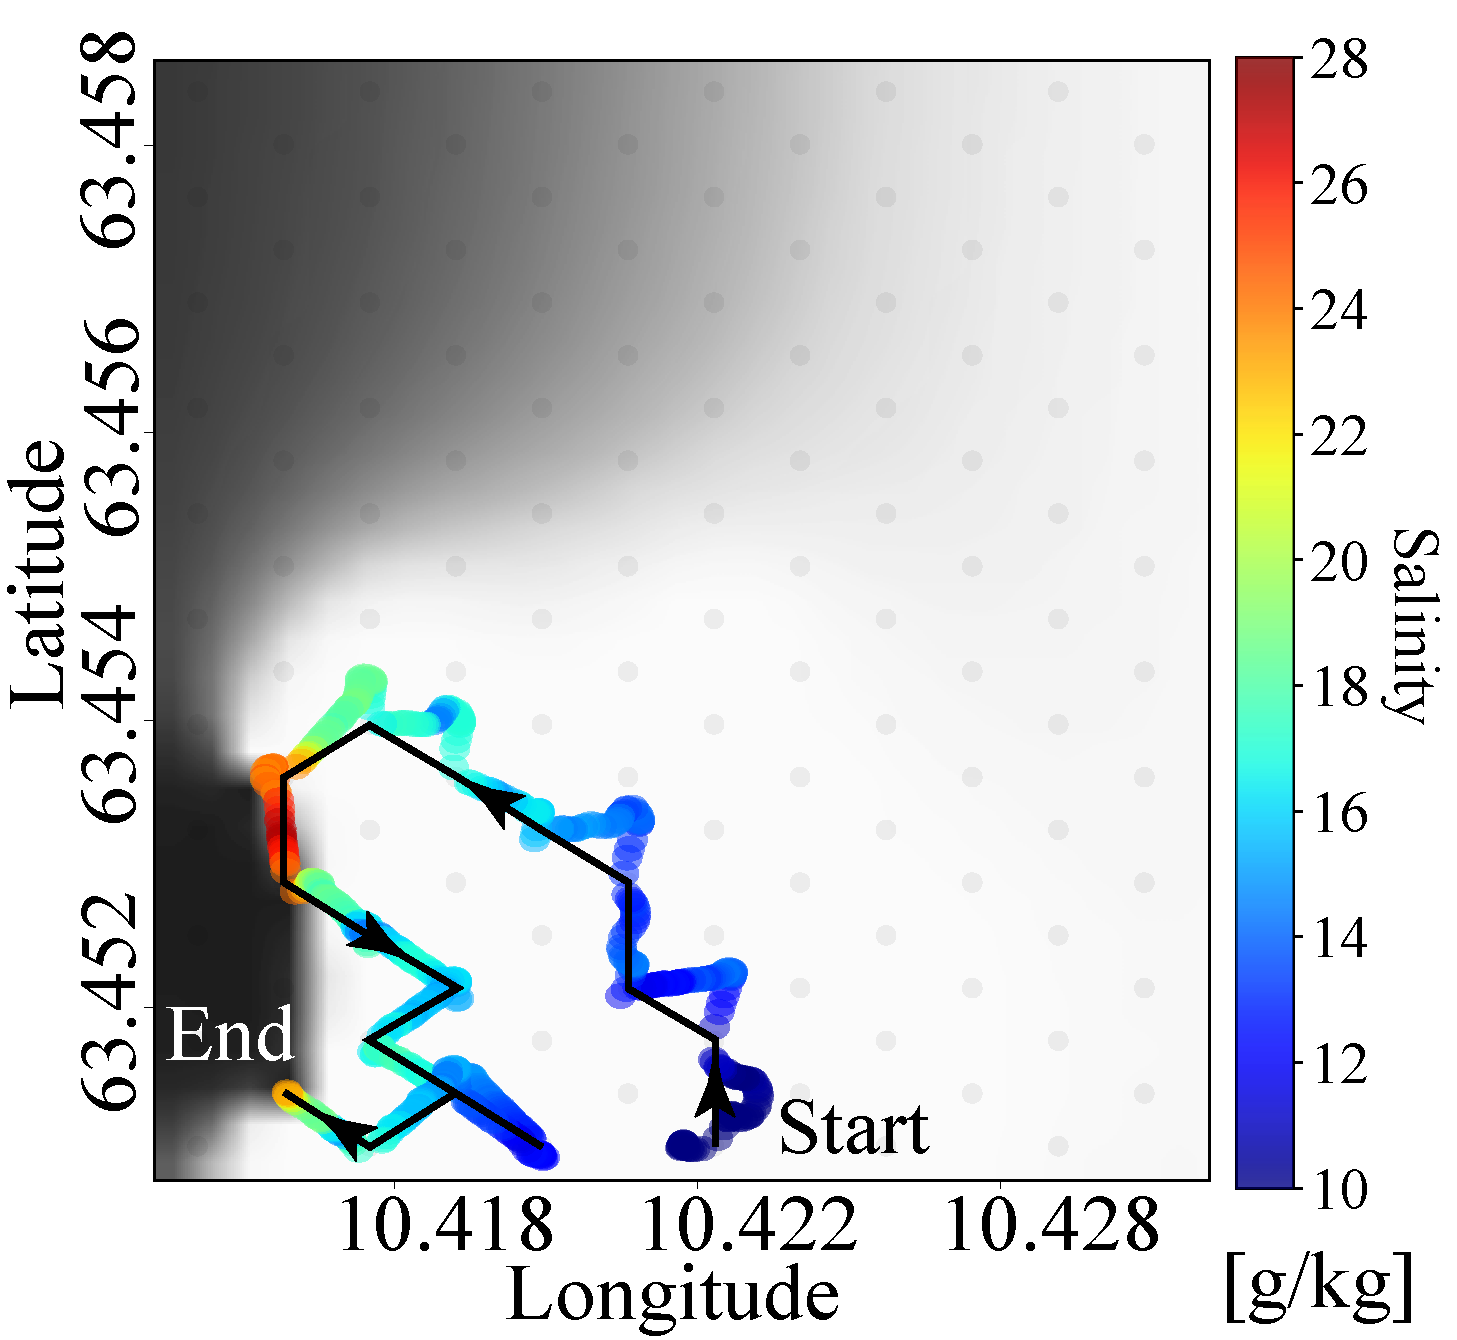
\includegraphics[height=0.40\textwidth]{Figures/field-trials/auv4_es_sal.pdf}\label{fig:res2}}

\subfigure[ES for Survey 1.]{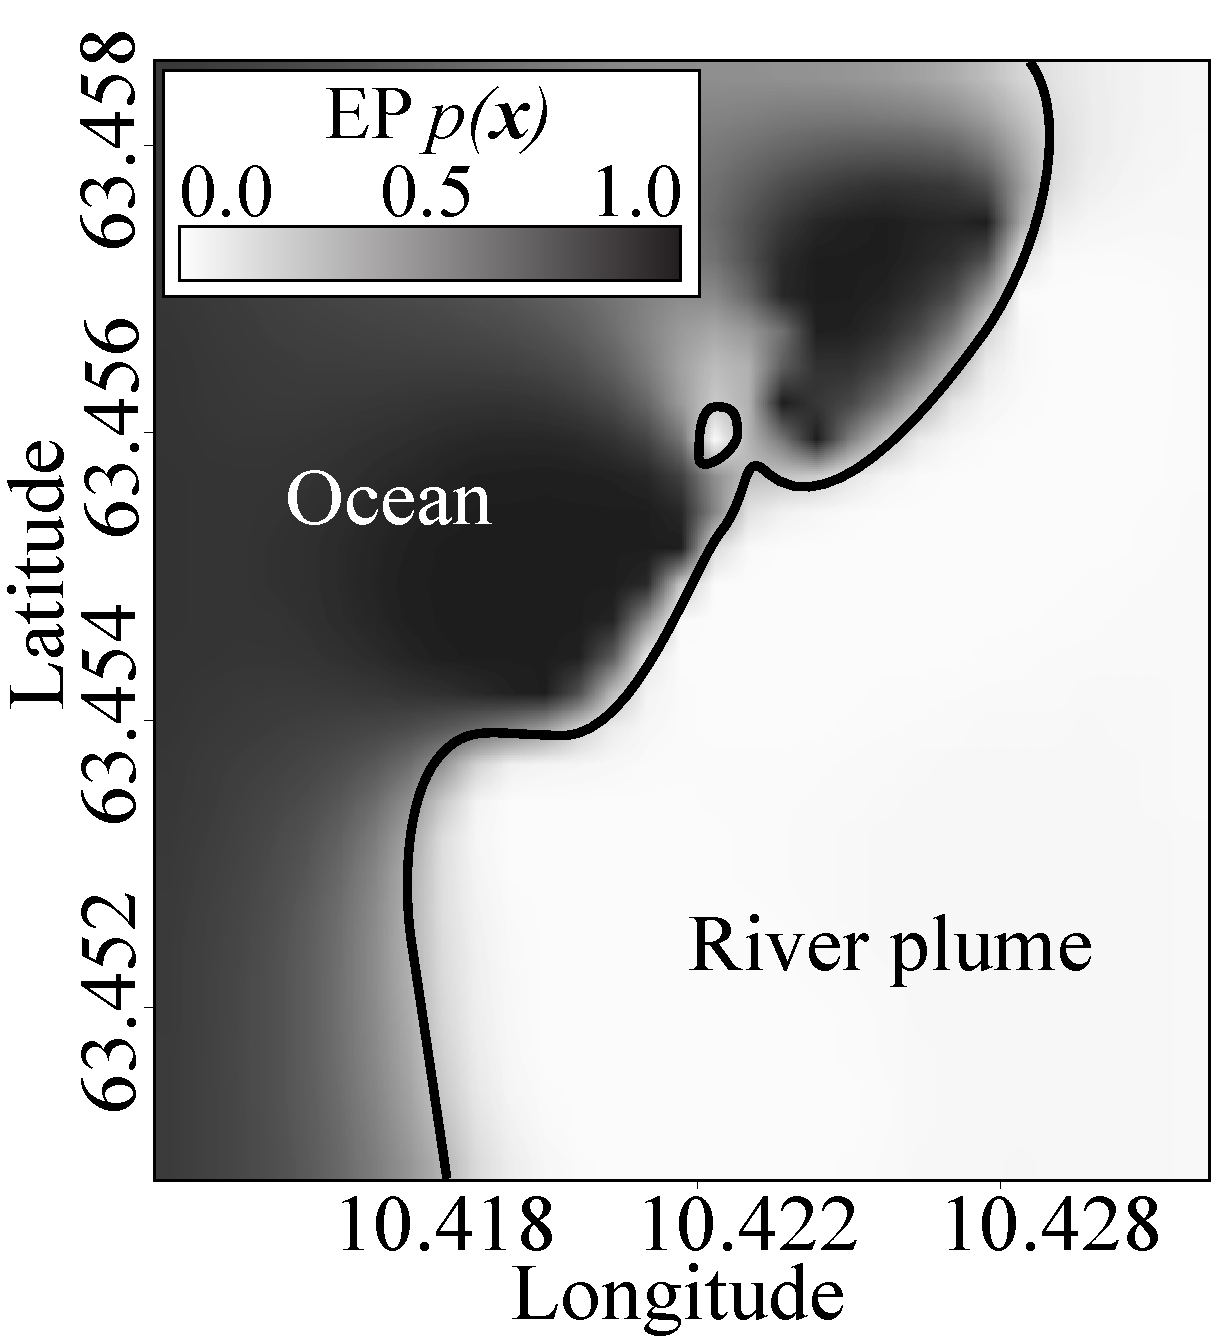
\includegraphics[height=0.41\textwidth]{Figures/field-trials/ep_1.pdf}\label{fig:res3}}\hspace{0.4cm}
\subfigure[ES for Survey 2.]{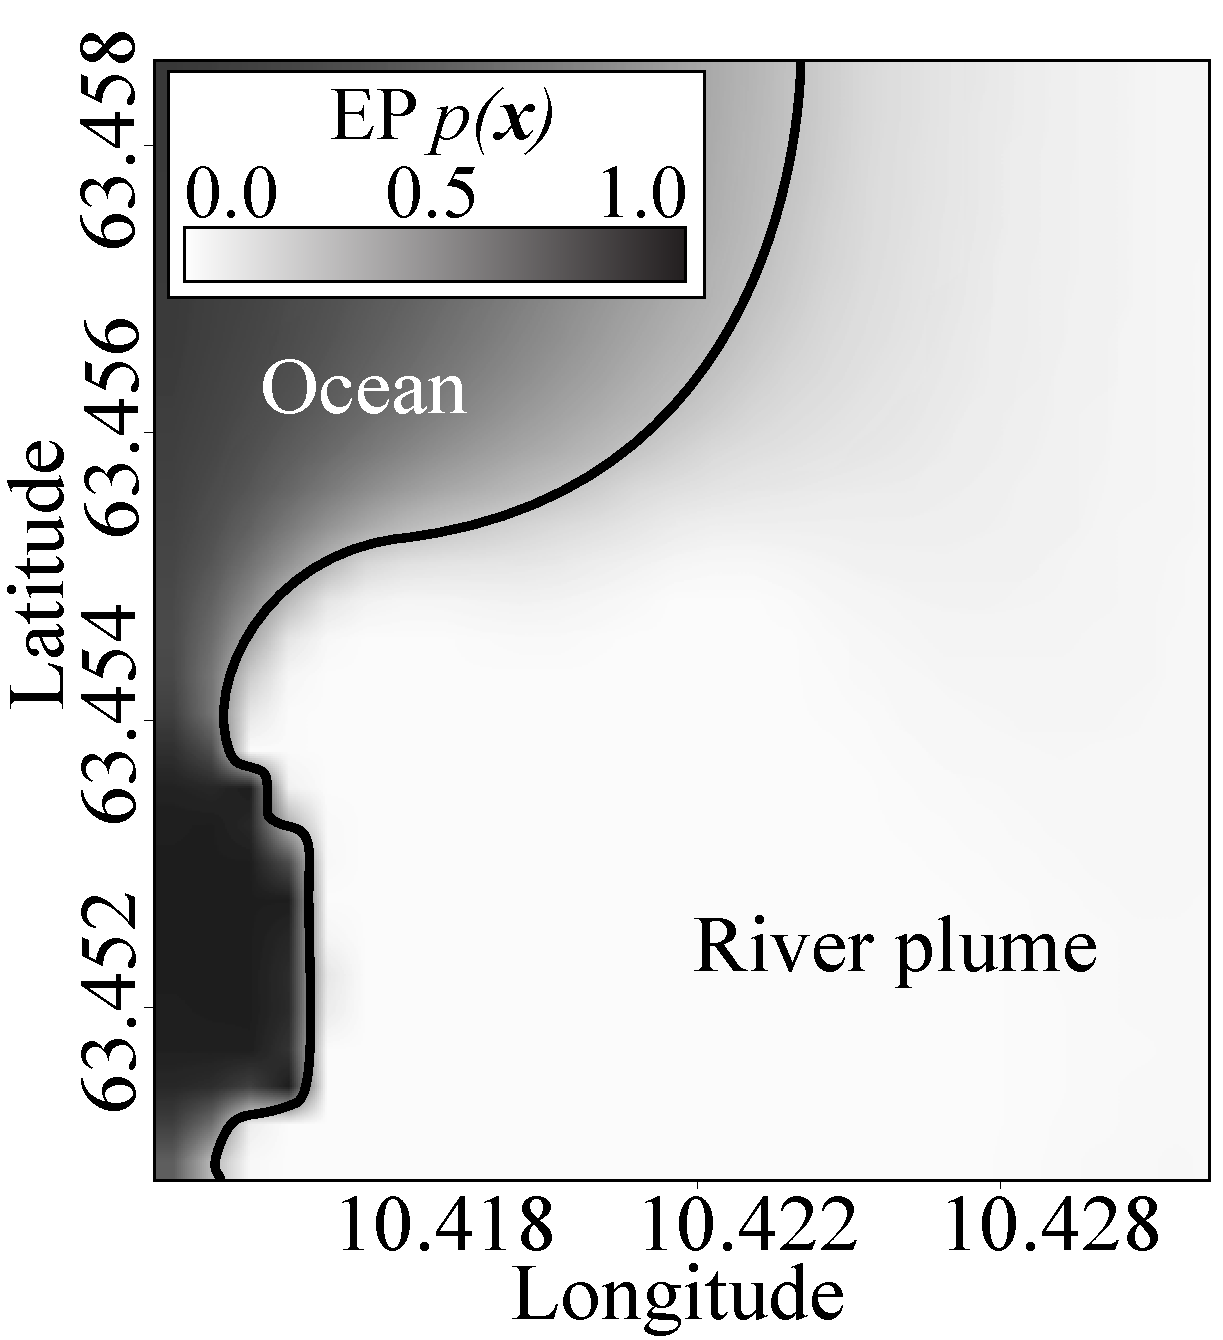
\includegraphics[height=0.41\textwidth]{Figures/field-trials/ep_4.pdf}\label{fig:res4}}
\caption{Results from mapping the Nidelven river} 
\label{fig:results}
\end{figure*}

\subsection{Results}

Two missions, Survey 1 and 2, were run successively from 11:00 AM to 01:00 PM, with a short break in between. The resulting path of the selected waypoints are shown in the map in Fig. \ref{fig:map}, both within the expected frontal region (shaded pink region). The recorded temperatures are shown as colored trails in Fig. \ref{fig:res_both}, clearly showing the temperature difference between fjord and river waters. The salinity data are then shown separately overlaid with the estimated EP for each survey in Fig. \ref{fig:res1} and \ref{fig:res2}. 

Both Survey 1 and 2 successfully estimate and navigate the separation zone crossing the frontal boundary multiple times. As conditions changed slightly between the two deployments the resulting path (after waypoint 5) deviates. Survey 1 continues northwards tracking the north-eastern part of the front, while Survey 2 turns west mapping the south-western part. 

The final prediction of the front location given in Fig. \ref{fig:res3} and \ref{fig:res4}, correspond with one another yielding a picture of the front gradually bending off towards north east. The amount of exploration done by Survey 1 is greater than Survey 2. In Survey 1 the AUV gets overall more detail by going north, while Survey 2 coming close to the survey area borders in the south-western corner get poorer understanding of the northern parts. A longer planning horizon would likely identify and discourage such choices.

%\begin{figure}[!h] 
% \centering 
%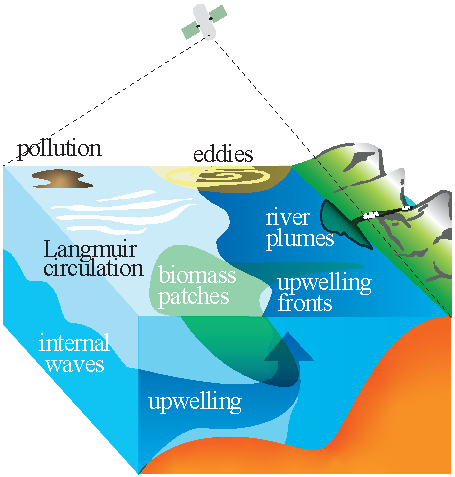
\includegraphics[width=0.48\textwidth]{Figures/envir_ocean.pdf}
%\caption{Ocean observation is moving away from %single-ship sampling
%towards more collaborative networked operations in %order to resolve
%the numerous processes and their interaction.} %\label{fig:envir}
%\end{figure}

\section{Closing remarks}\label{sec:concl_disc}

This paper builds on multidisciplinary work combining statistical modeling and methods with robotic surveying technologies for oceanographic sensing applications. We show how the observation practices can gain from development of statistical techniques to achieve more effective spatial monitoring. We further demonstrate the opportunities available for real-time multivariable spatial data gathering and analysis onboard autonomous sensing platforms, upon which statisticians can exploit towards creating general-purpose toolkits for similar applications (enabeling theory).

In particular, we derive and show results for characterizing phenomena connected to water masses properties. The characterization is based on joint excursion sets and we derive new results for the expected integrated Bernoulli variance reduction achieved by the spatial sampling design. This result is first derived for the situation with a static design, and then extended to the adaptive situation, which provides new insight in our application with the autonomous vehicle.

The study did not consider any temporal effects, which would be relevant on a larger time scale. We consider the extension to spatio-temporal modeling as future work, and we envision that advection-diffusion equations could be useful in this kind of modeling \citep{sigrist2015stochastic}. For more complex oceanographic phenomena, the methods will need to be extended to non-Gaussian phenomena, possibly feature-based mixtures of GPs which could still be run onboard, and augmented by dynamical models. 

The spatial statistical design criterion building on excursion sets is relevant in our setting with the different water mass properties and could also be useful in other oceanographic settings such as algae-blooms or frontal systems. Other criteria more directly related to decision making would also be relevant, especially with much spatio-temporal effects. For instance, managers must make difficult decisions related to fish farming or other marine resources operations, or environmental projects. Value of information analysis \citep{Eidsvik:15} would then be used in a similar vein as the integrated Bernoulli variance in the current paper, now studying which, when and where information is likely to materialize in improved decisions. 

While more effort could be spent on approximating the look-ahead steps, it is perhaps more interesting to explore the additional flexibility that can be gained by having two or more AUVs \citep{ferreira2019advancing} exploring a spatial or spatio-temporal domain together. It might then be useful to sample different parts of the space, and maybe move in parallel to best capture the excursion set.

\section*{Acknowledgements}
TOF and KR acknowledge support from the Centre for Autonomous Marine Operations and Systems (AMOS)\footnote{\url{https://www.ntnu.edu/amos}}, Center of Excellence, project number 223254, and the Applied Underwater Robotics Labortatory (AURLab). JE acknowledge support from Norwegian research council project 294404. DG acknowledges support from the Swiss National Science Foundation project number 178858.

%\begin{supplement}
%\sname{Supplement A}\label{suppA}
%\stitle{Title of the Supplement A}
%\slink[url]{http://www.e-publications.org/ims/support/dowload/imsart-ims.zip}
%\sdescription{Dum esset rex in
%accubitu suo, nardus mea dedit odorem suavitatis. Quoniam confortavit
%seras portarum tuarum, benedixit filiis tuis in te. Qui posuit fines tuos}
%\end{supplement}

% == Adding references
\footnotesize
\bibliographystyle{apalike}
\bibliography{ref}

% AOS,AOAS: If there are supplements please fill:
%\begin{supplement}[id=suppA]
%  \sname{Supplement A}
%  \stitle{Title}
%  \slink[doi]{10.1214/00-AOASXXXXSUPP}
%  \sdatatype{.pdf}" 
%  \sdescription{Some text}
%\end{supplement}

\end{document}
